\chapter{Selection Binning}\label{app:bintemplates}

Templates for the non-uniform fit binning for each sample are presented in this section, as it is not feasible to express the bin edges in text for non-uniform binning. Figure \ref{fig:th2polybinreset5000} shows the x-axis range reduced to 0-5000 MeV so that the smaller bins in the peak can be seen. Figure \ref{fig:th2polybinreset} shows the full distributions out to 30 GeV, for each sample.

\begin{figure}
\centering
\begin{subfigure}{.32\textwidth}
  \centering
  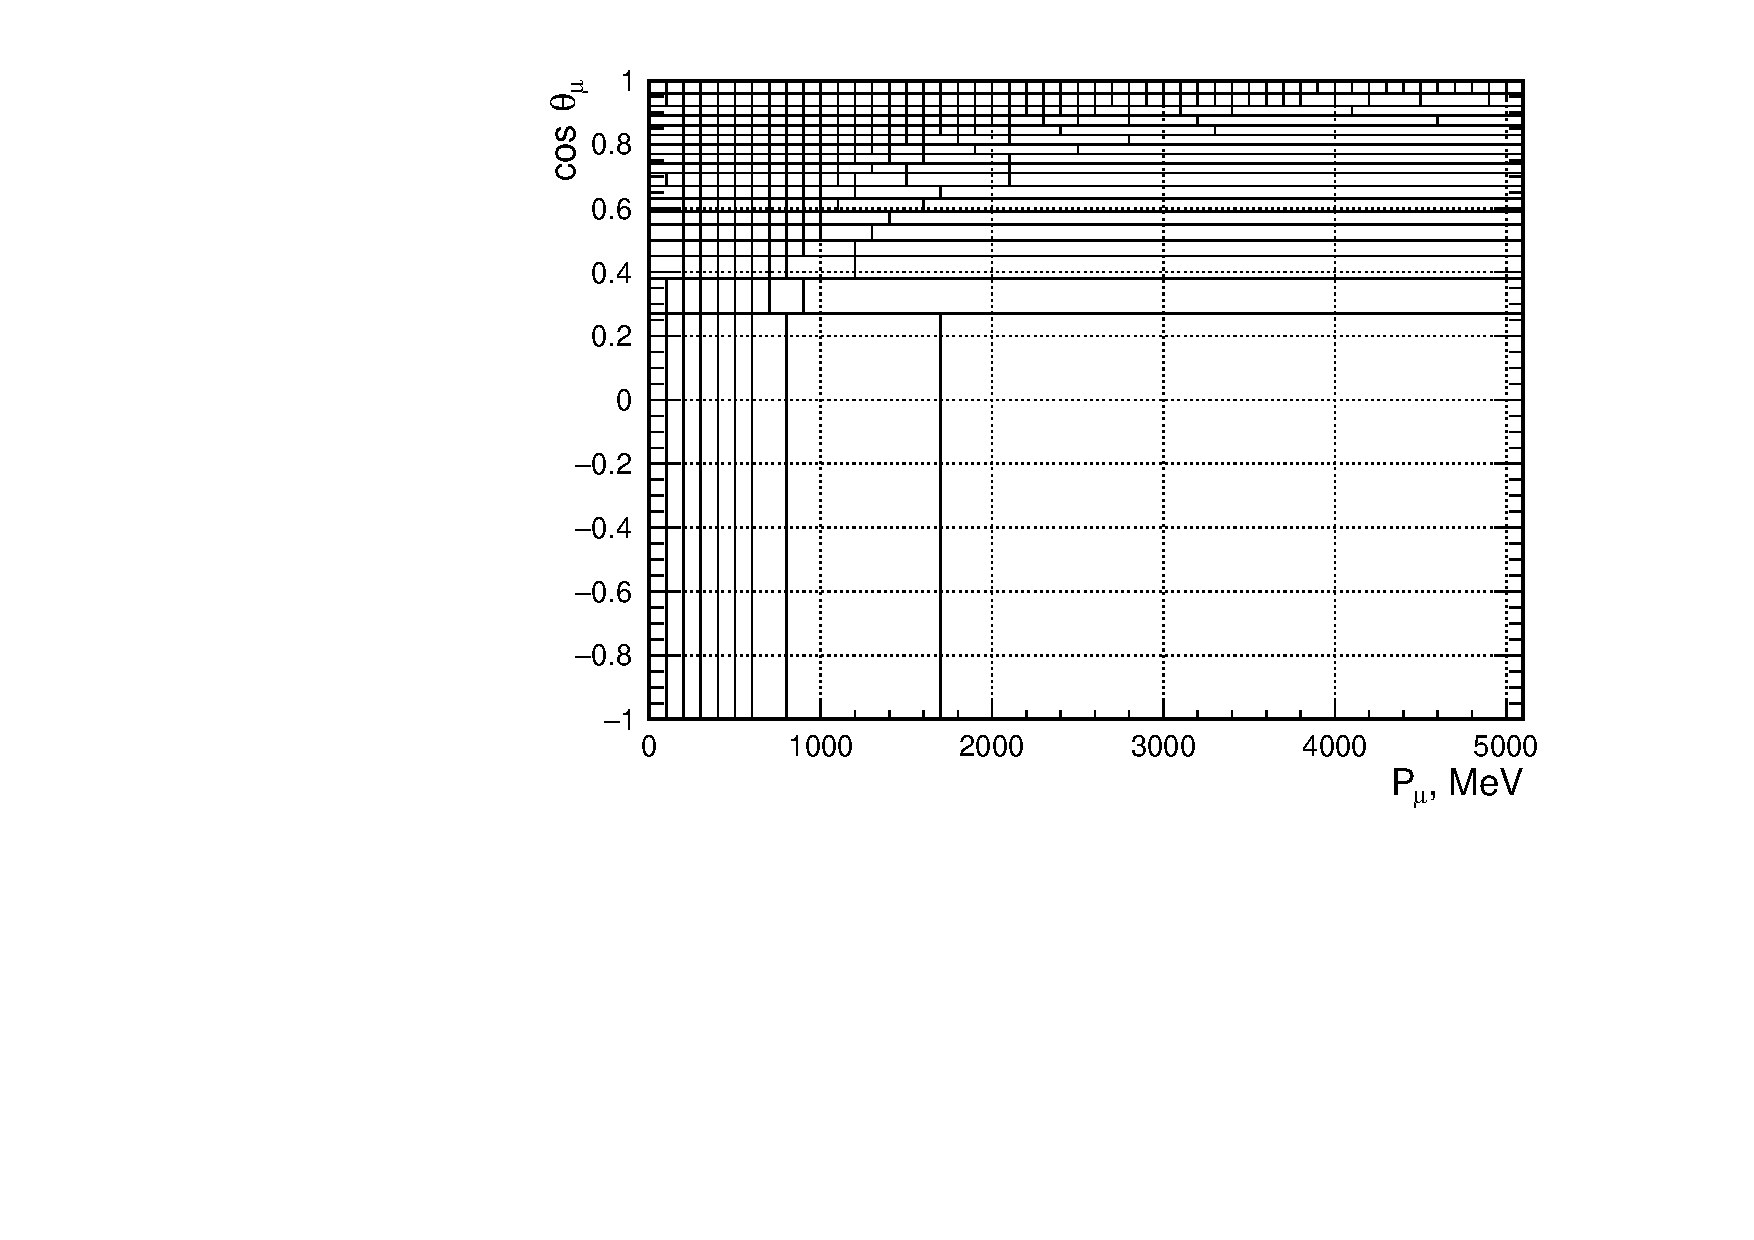
\includegraphics[width=0.95\linewidth]{figs/TH2PolyReset5000_MC_FGD1_numuCC_0pi}
  \caption{FGD1 FHC $\nu_{\mu}$ 0$\pi$}
  \label{fig:TH2Poly_Reset5000FGD1_numuCC_0pi}
\end{subfigure}
\begin{subfigure}{.32\textwidth}
  \centering
  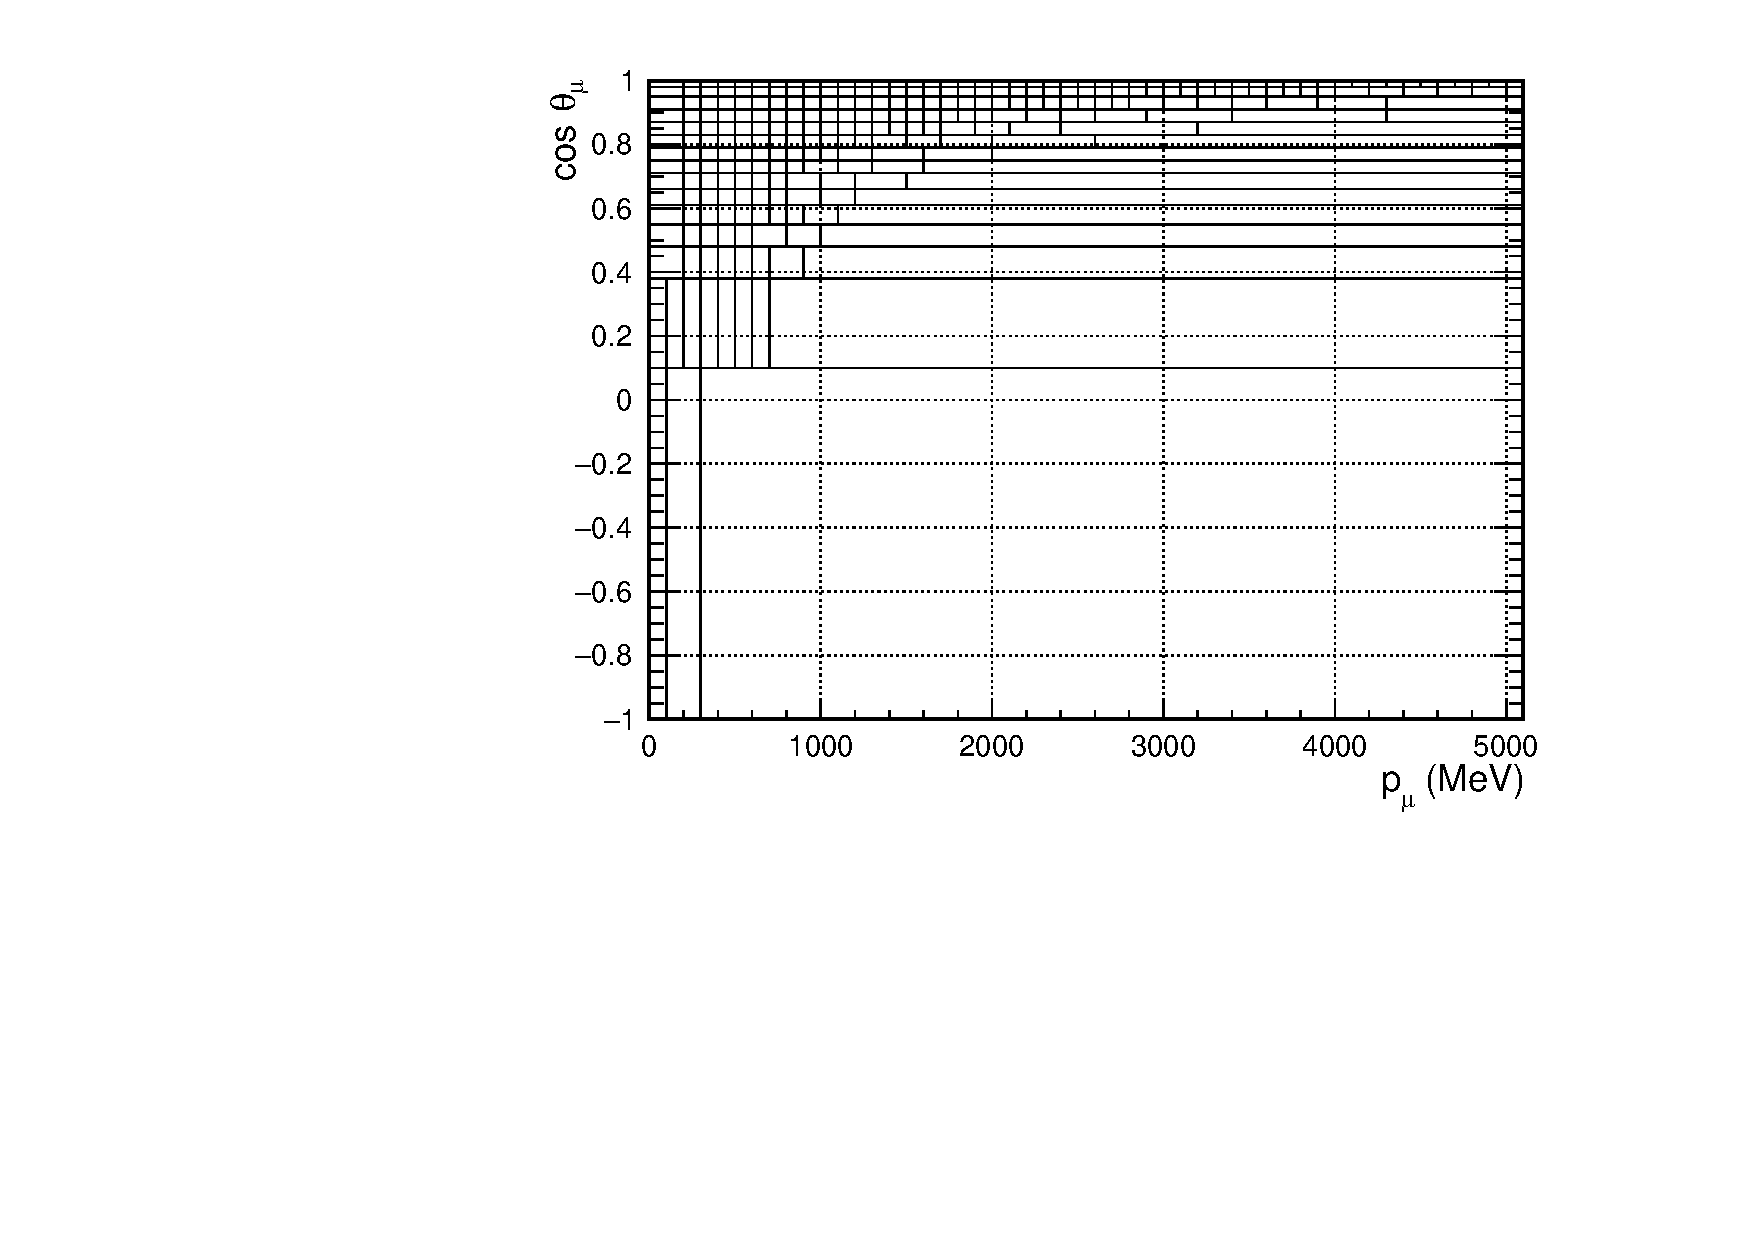
\includegraphics[width=0.95\linewidth]{figs/TH2PolyReset5000_MC_FGD1_numuCC_1pi}
  \caption{FGD1 FHC $\nu_{\mu}$ 1$\pi$}
  \label{fig:TH2Poly_Reset5000FGD1_numuCC_1pi}
\end{subfigure}
\begin{subfigure}{.32\textwidth}
  \centering
  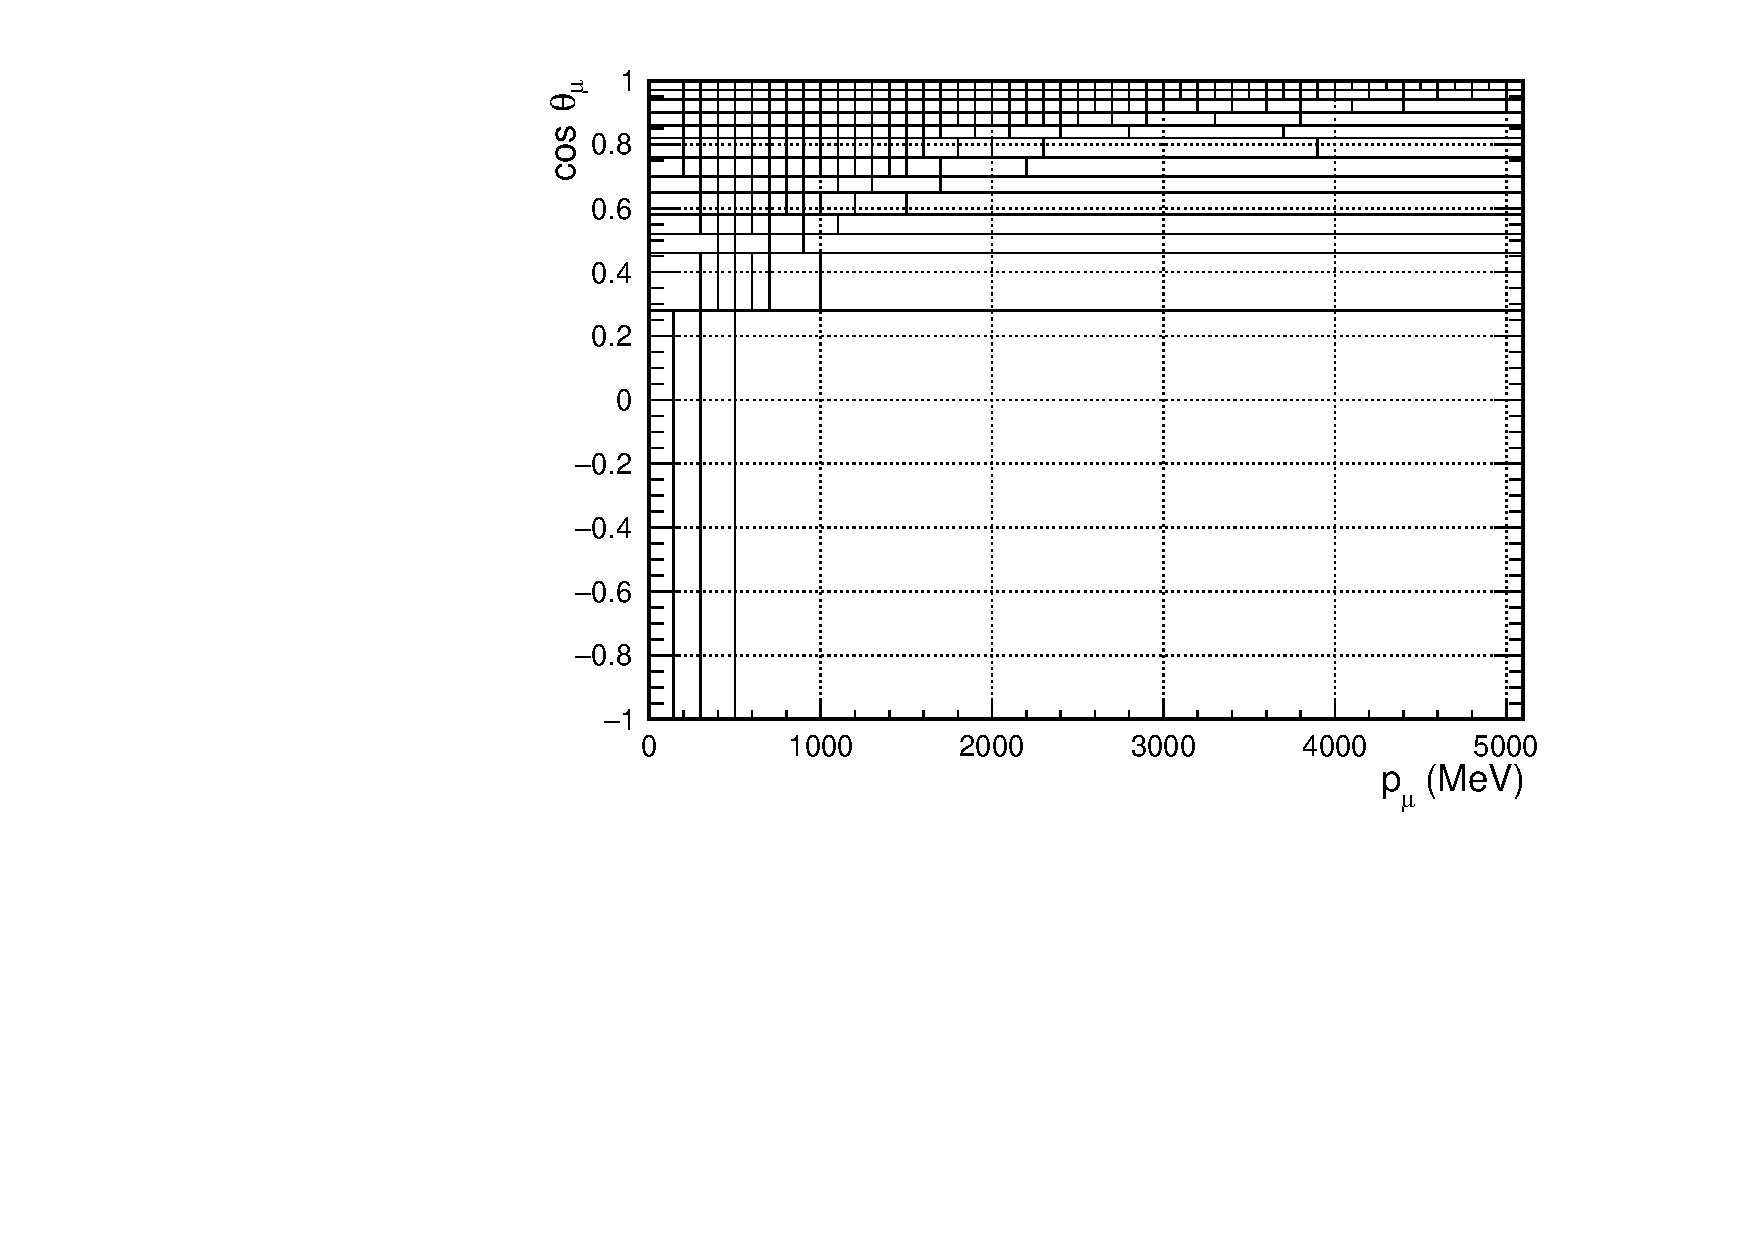
\includegraphics[width=0.95\linewidth]{figs/TH2PolyReset5000_MC_FGD1_numuCC_other}
  \caption{FGD1 FHC $\nu_{\mu}$ Other}
  \label{fig:TH2Poly_Reset5000FGD1_numuCC_other}
\end{subfigure}
\centering
\begin{subfigure}{.32\textwidth}
  \centering
  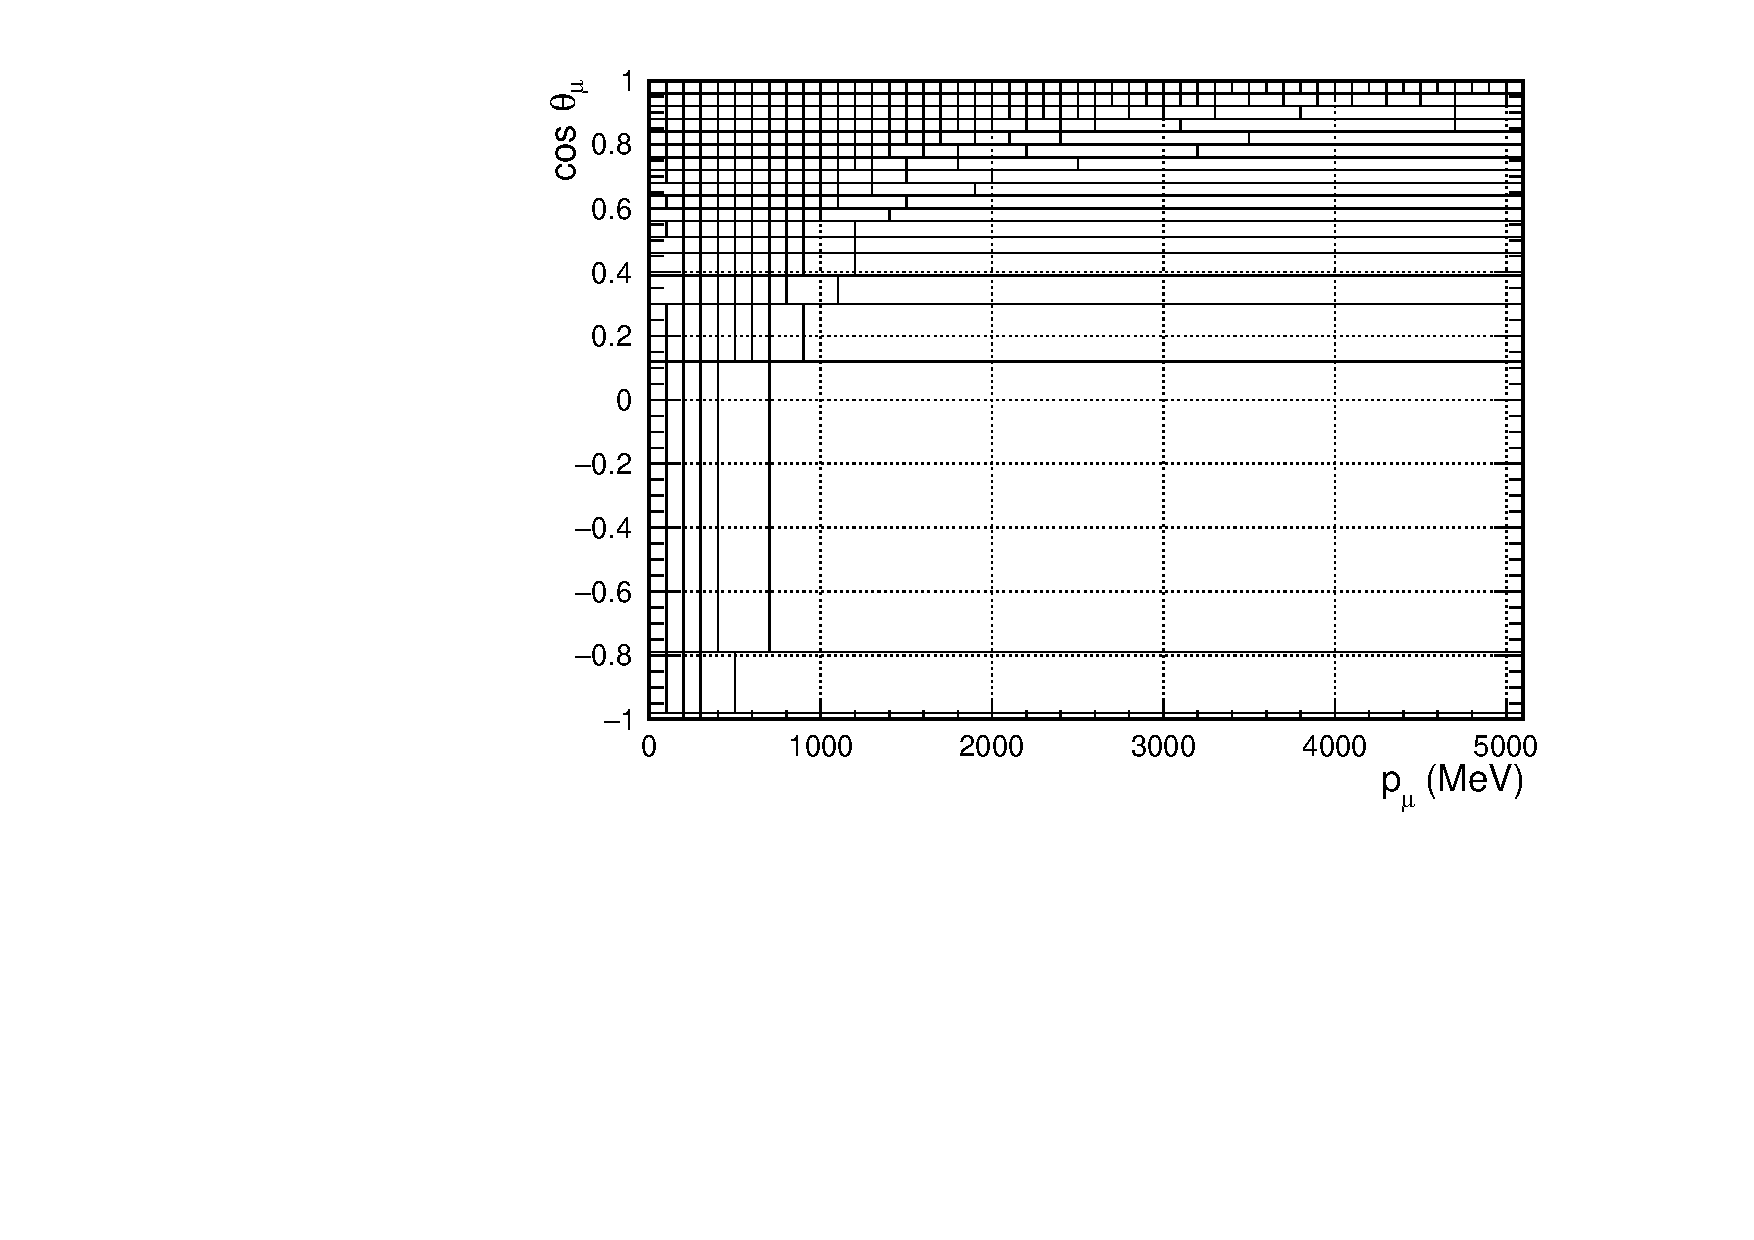
\includegraphics[width=0.95\linewidth]{figs/TH2PolyReset5000_MC_FGD2_numuCC_0pi}
  \caption{FGD2 FHC $\nu_{\mu}$ 0$\pi$}
  \label{fig:TH2Poly_Reset5000FGD2_numuCC_0pi}
\end{subfigure}
\begin{subfigure}{.32\textwidth}
  \centering
  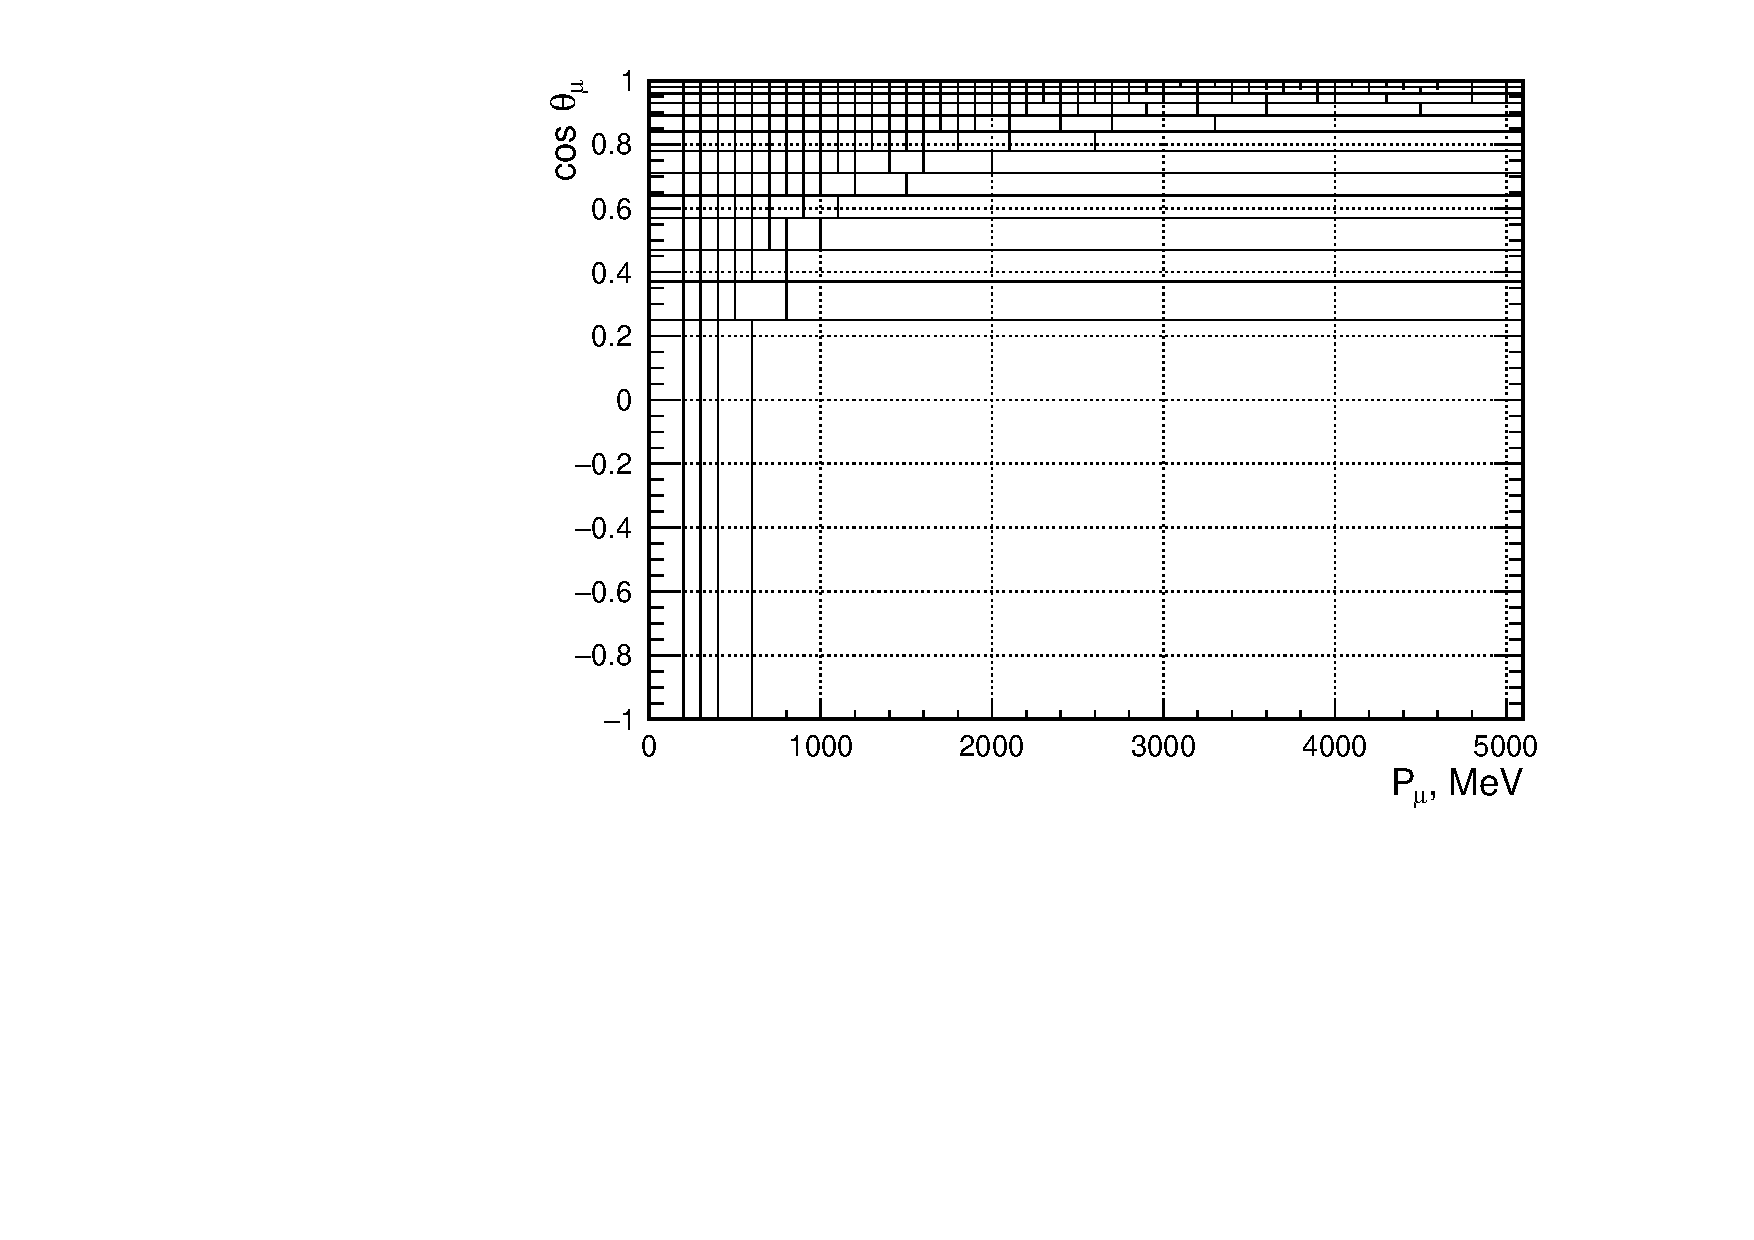
\includegraphics[width=0.95\linewidth]{figs/TH2PolyReset5000_MC_FGD2_numuCC_1pi}
  \caption{FGD2 FHC $\nu_{\mu}$ 1$\pi$}
  \label{fig:TH2Poly_Reset5000FGD2_numuCC_1pi}
\end{subfigure}
\begin{subfigure}{.32\textwidth}
  \centering
  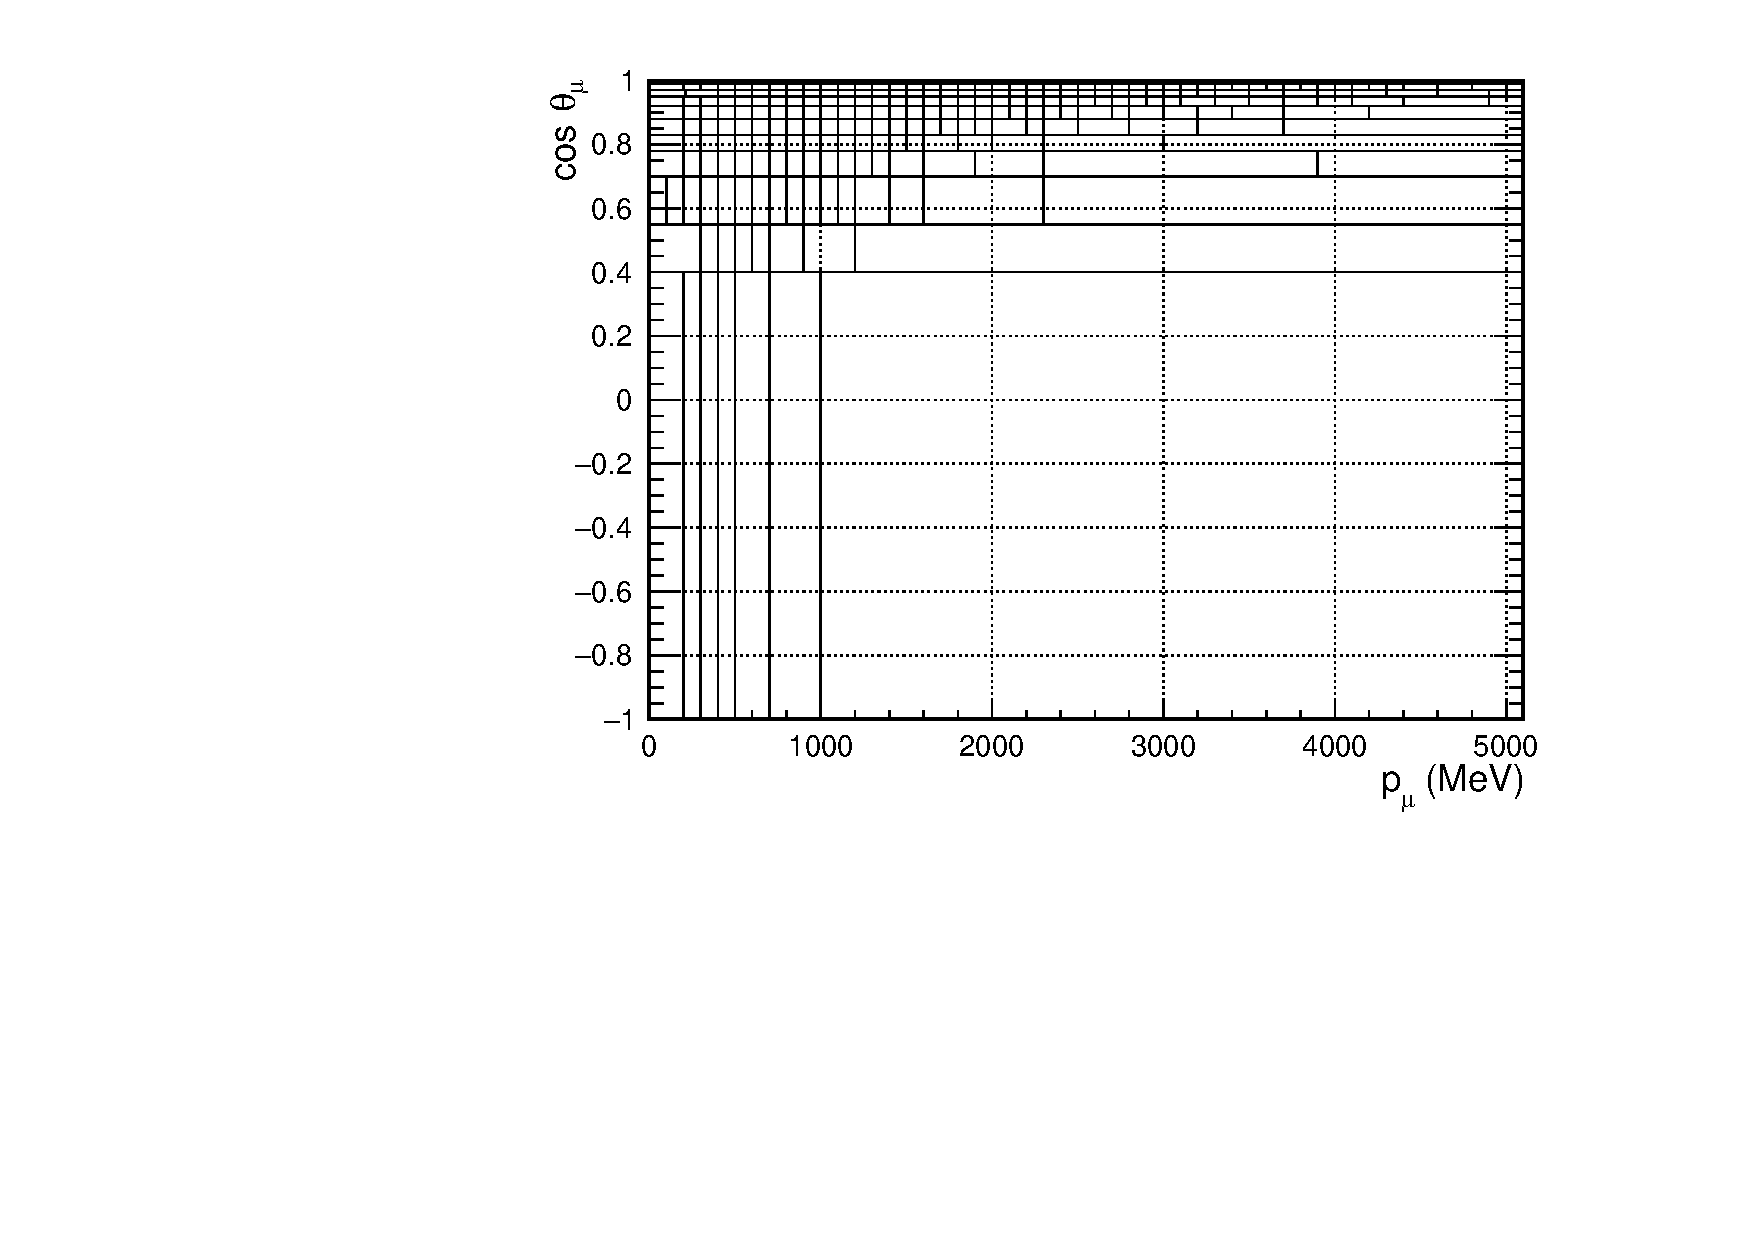
\includegraphics[width=0.95\linewidth]{figs/TH2PolyReset5000_MC_FGD2_numuCC_other}
  \caption{FGD2 FHC $\nu_{\mu}$ Other}
  \label{fig:TH2Poly_Reset5000FGD2_numuCC_other}
\end{subfigure}
\centering
\begin{subfigure}{.32\textwidth}
  \centering
  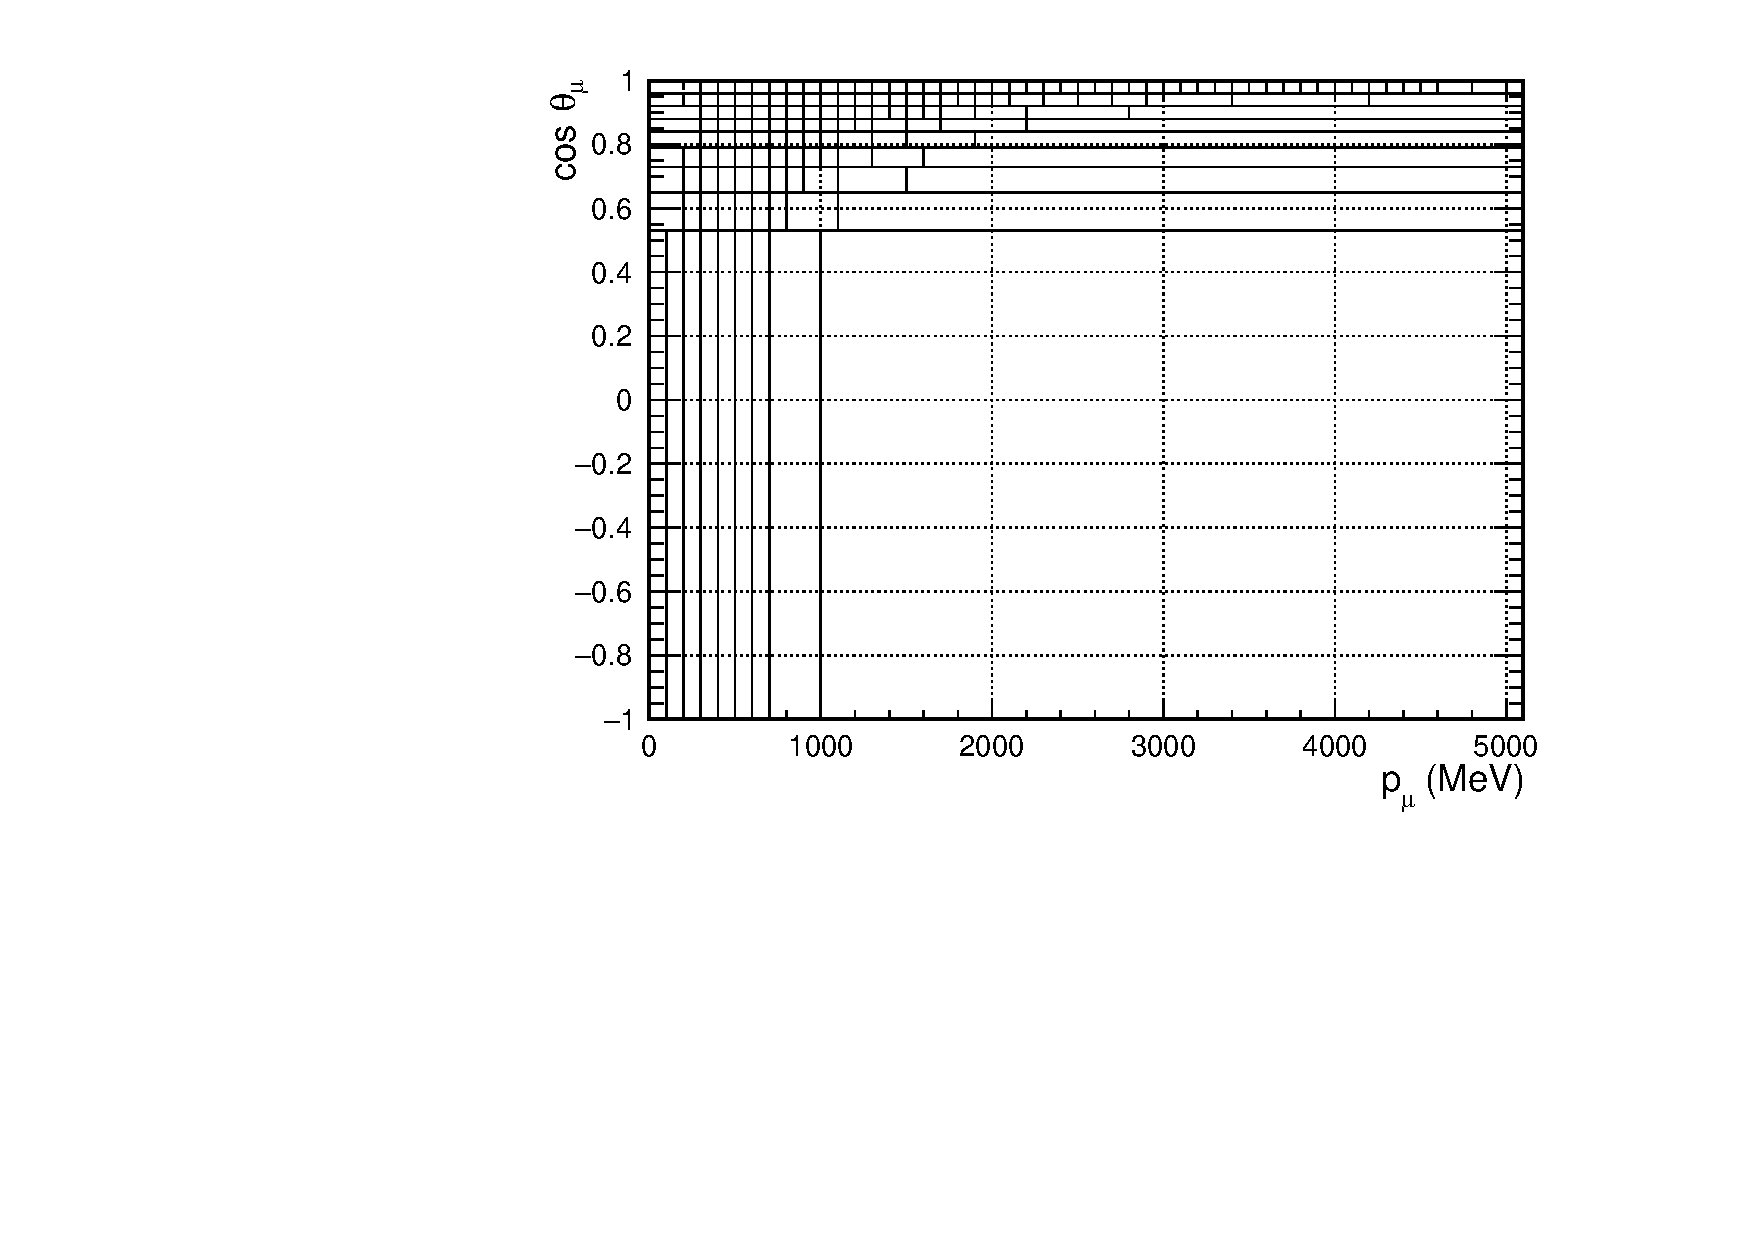
\includegraphics[width=0.95\linewidth]{figs/TH2PolyReset5000_MC_FGD1_anti-numuCC_0pi}
  \caption{FGD1 RHC $\bar{\nu_{\mu}}$ 0$\pi$}
  \label{fig:TH2Poly_Reset5000FGD1_anti-numuCC_0pi}
\end{subfigure}
\begin{subfigure}{.32\textwidth}
  \centering
  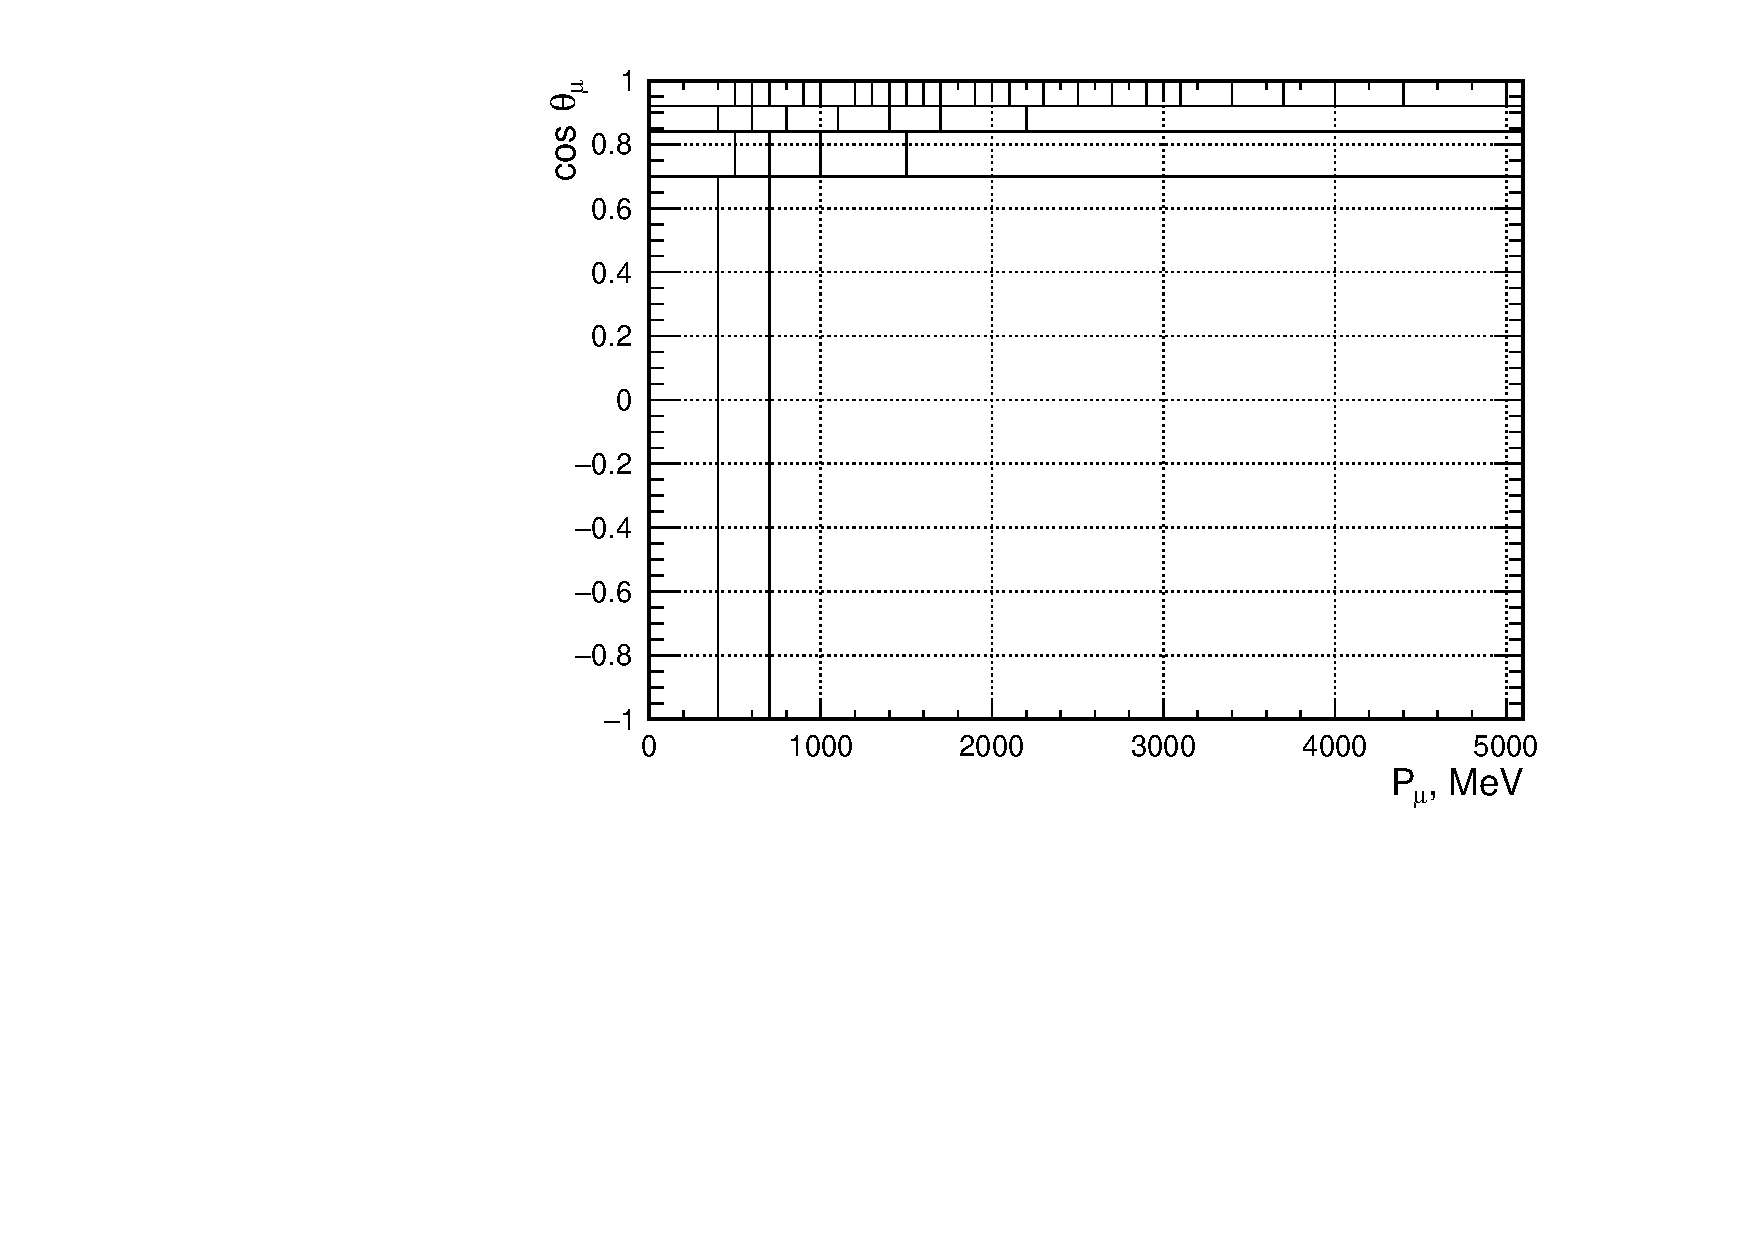
\includegraphics[width=0.95\linewidth]{figs/TH2PolyReset5000_MC_FGD1_anti-numuCC_1pi}
  \caption{FGD1 RHC $\bar{\nu_{\mu}}$ 1$\pi$}
  \label{fig:th2polyTH2Poly_Reset5000FGD1_anti-numuCC_1pi}
\end{subfigure}
\begin{subfigure}{.32\textwidth}
  \centering
  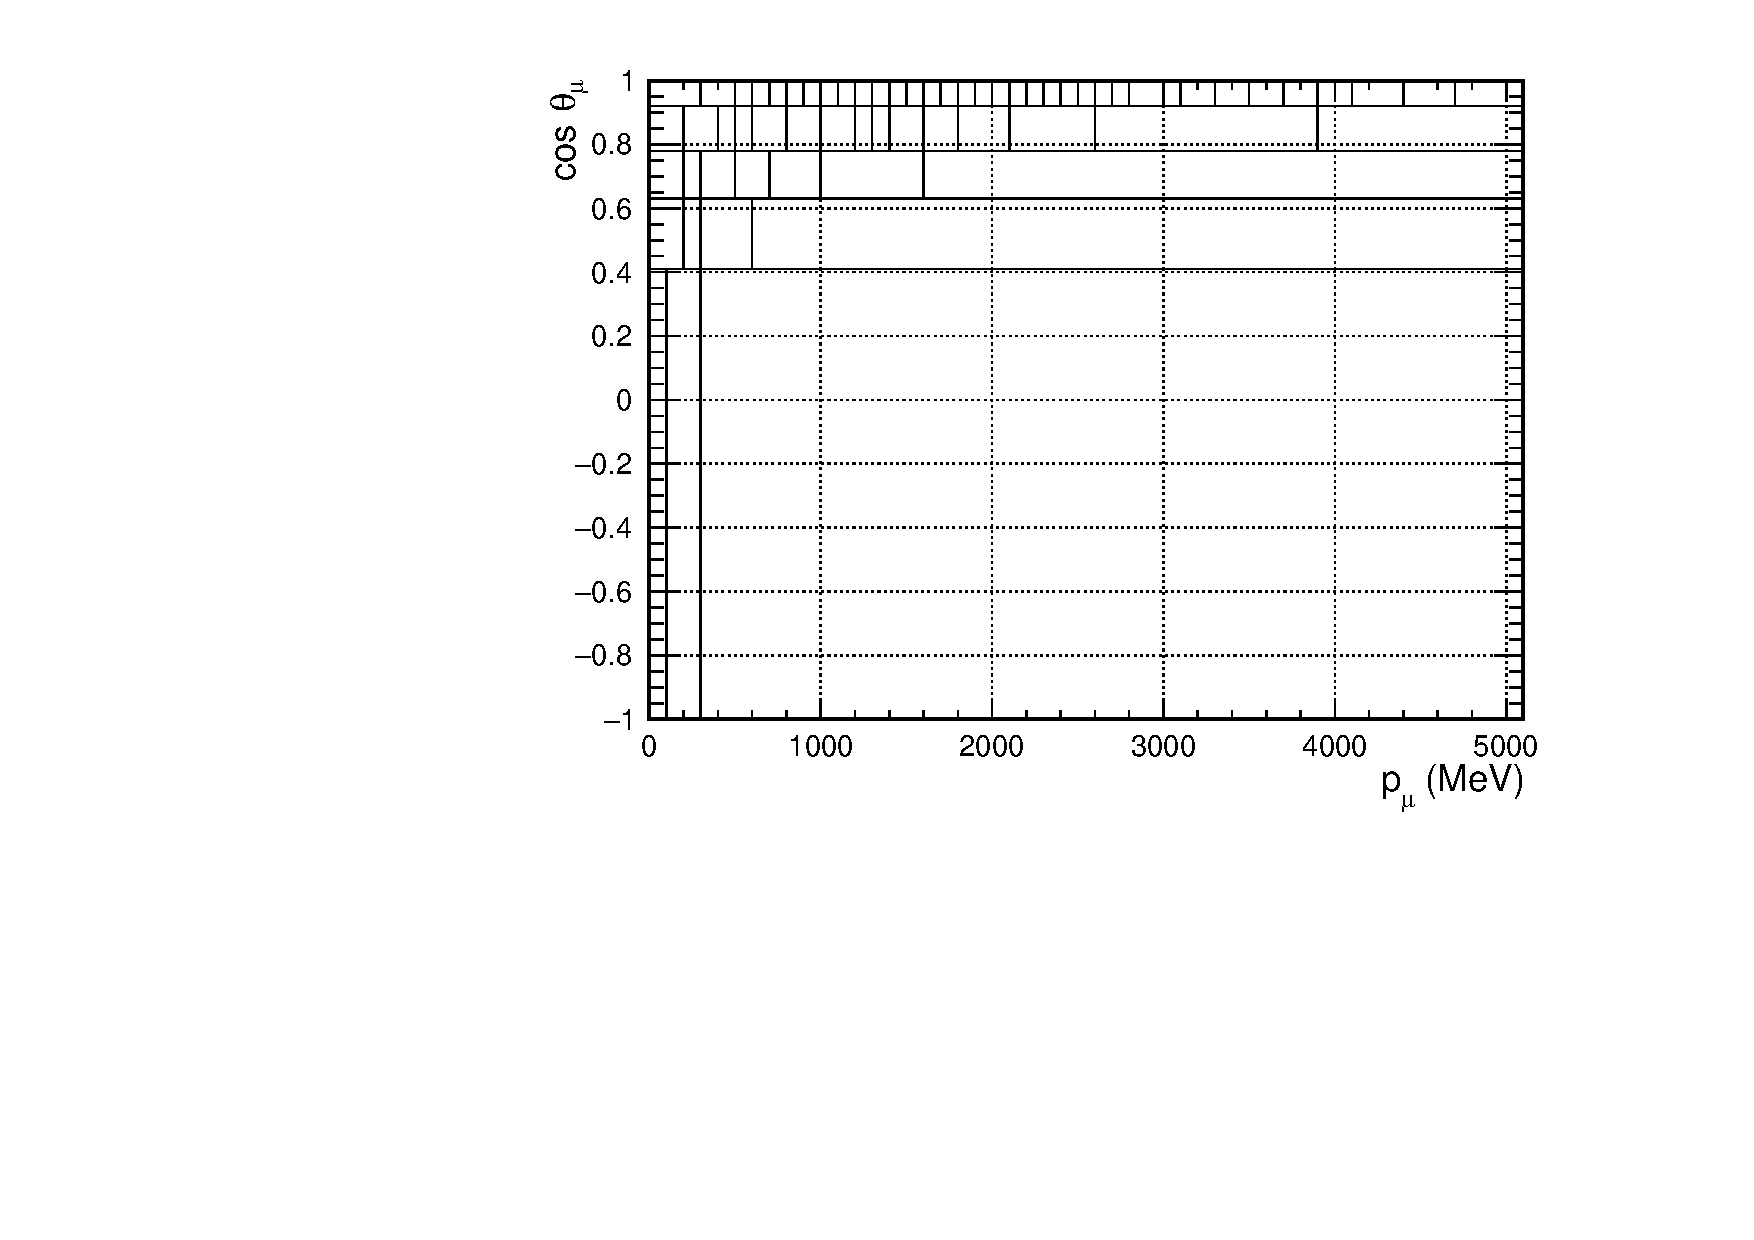
\includegraphics[width=0.95\linewidth]{figs/TH2PolyReset5000_MC_FGD1_anti-numuCC_other}
  \caption{FGD1 RHC $\bar{\nu_{\mu}}$ Other}
  \label{fig:TH2Poly_Reset5000FGD1_anti-numuCC_other}
\end{subfigure}
\centering
\begin{subfigure}{.32\textwidth}
  \centering
  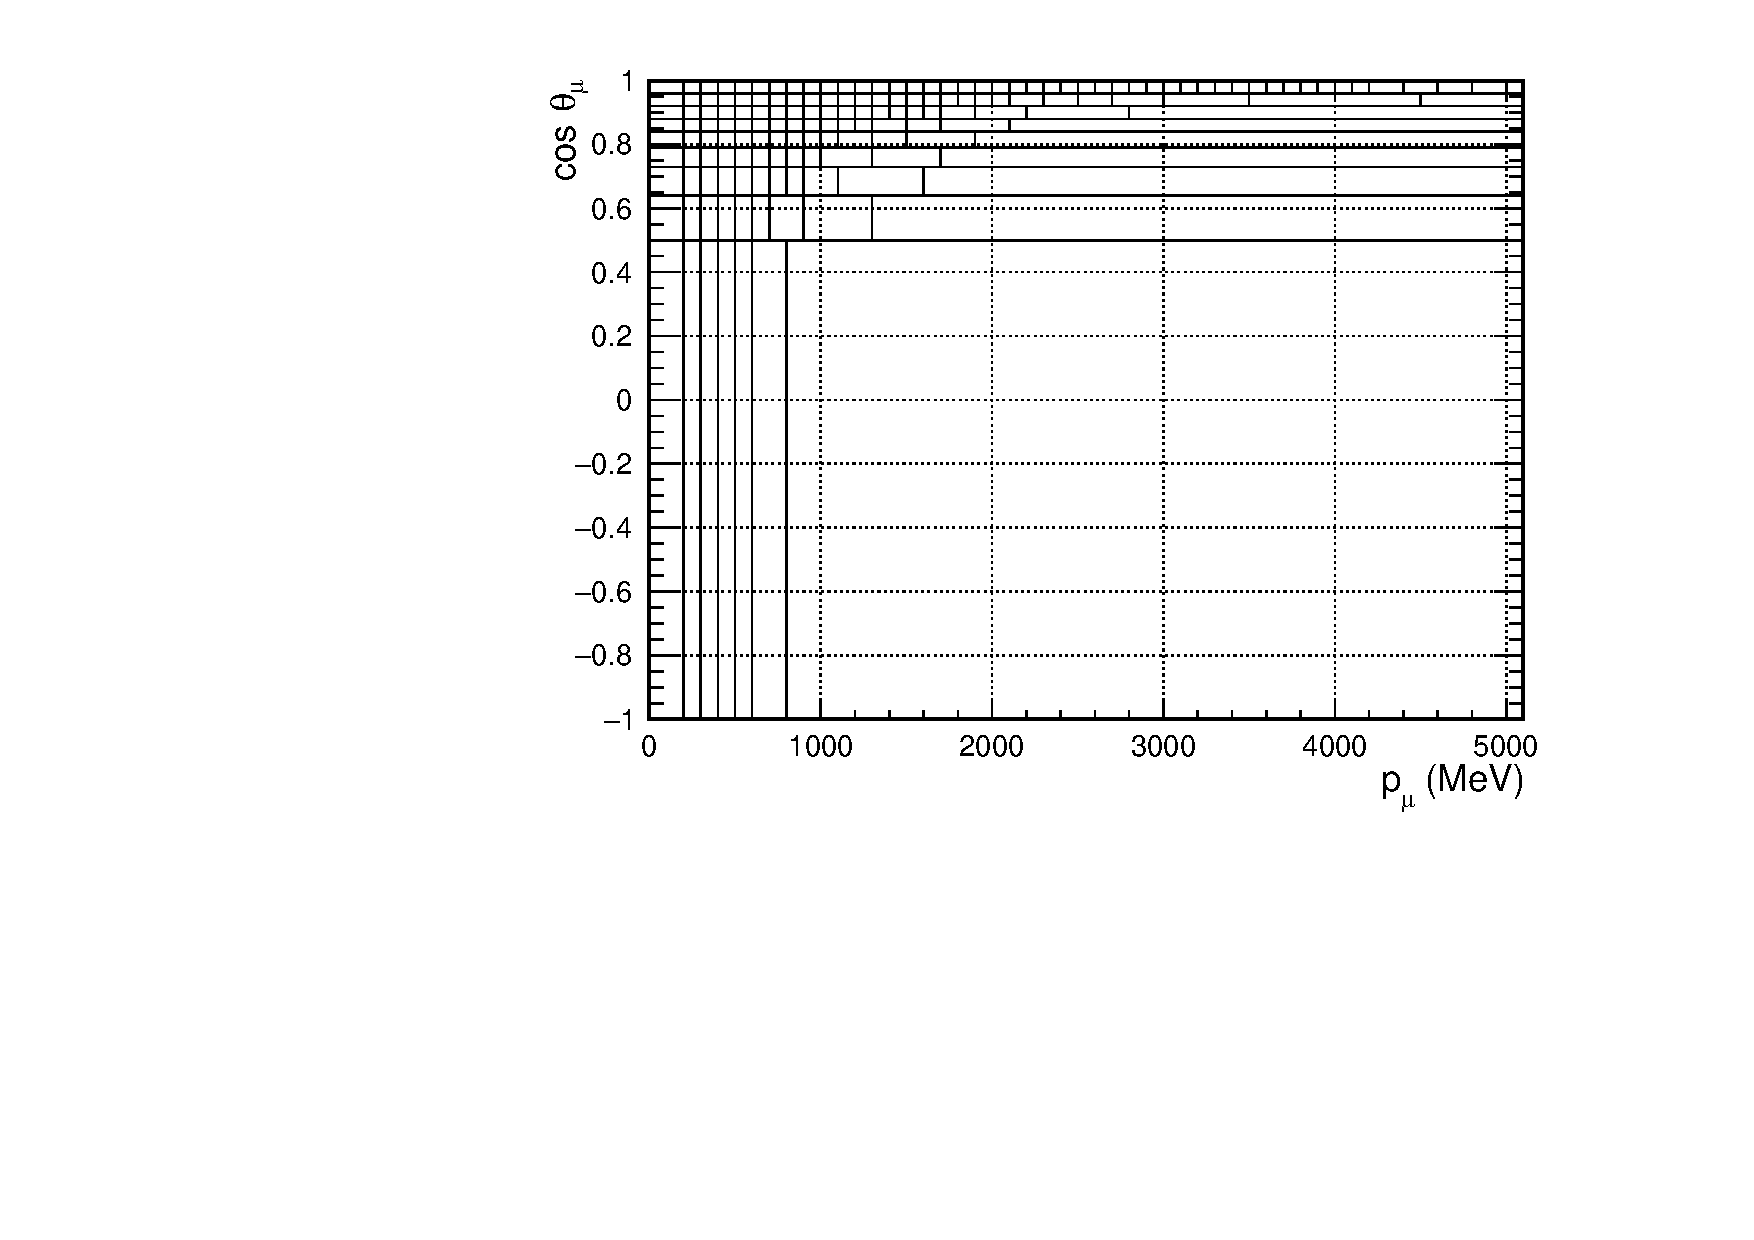
\includegraphics[width=0.95\linewidth]{figs/TH2PolyReset5000_MC_FGD2_anti-numuCC_0pi}
  \caption{FGD2 RHC $\bar{\nu_{\mu}}$ 0$\pi$}
  \label{fig:TH2Poly_Reset5000FGD2_anti-numuCC_0pi}
\end{subfigure}
\begin{subfigure}{.32\textwidth}
  \centering
  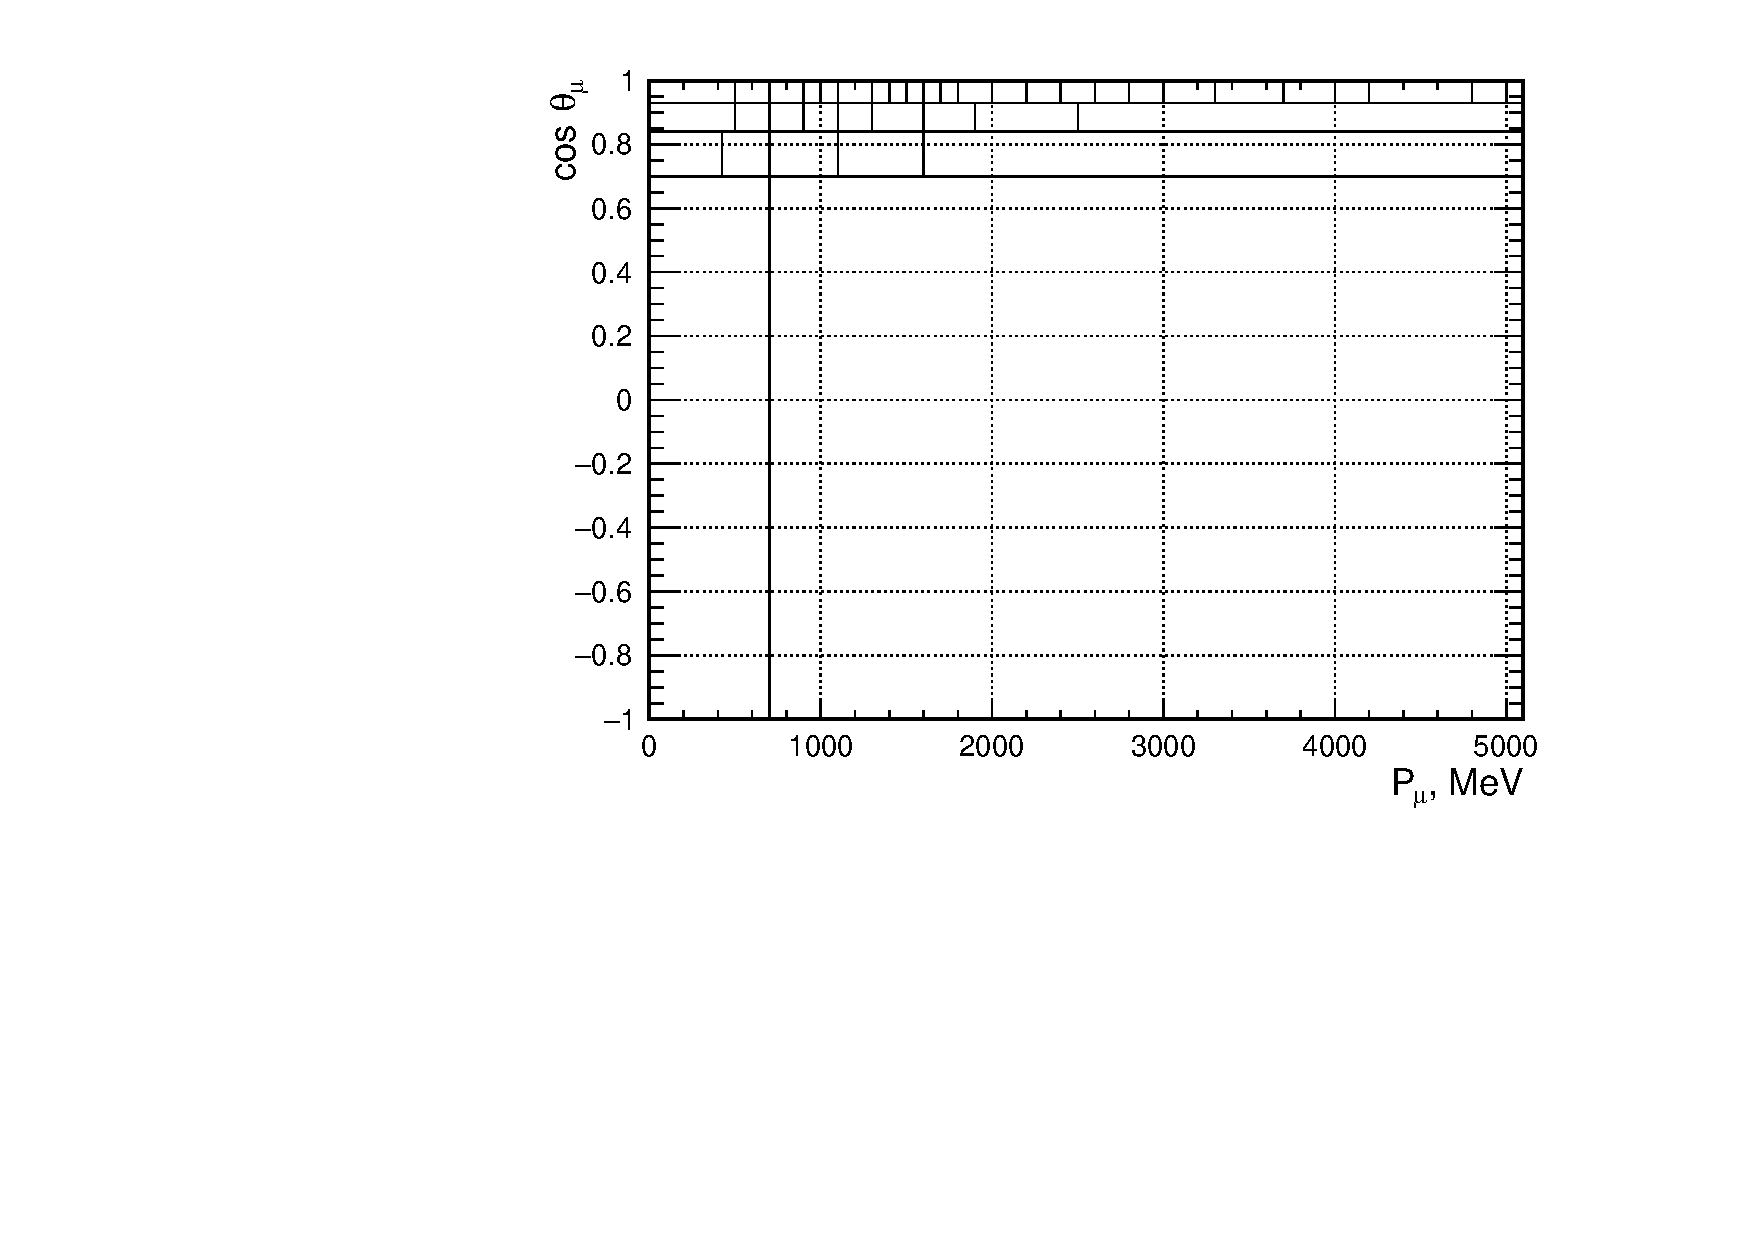
\includegraphics[width=0.95\linewidth]{figs/TH2PolyReset5000_MC_FGD2_anti-numuCC_1pi}
  \caption{FGD2 RHC $\bar{\nu_{\mu}}$ 1$\pi$}
  \label{fig:th2polyTH2Poly_Reset5000FGD2_anti-numuCC_1pi}
\end{subfigure}
\begin{subfigure}{.32\textwidth}
  \centering
  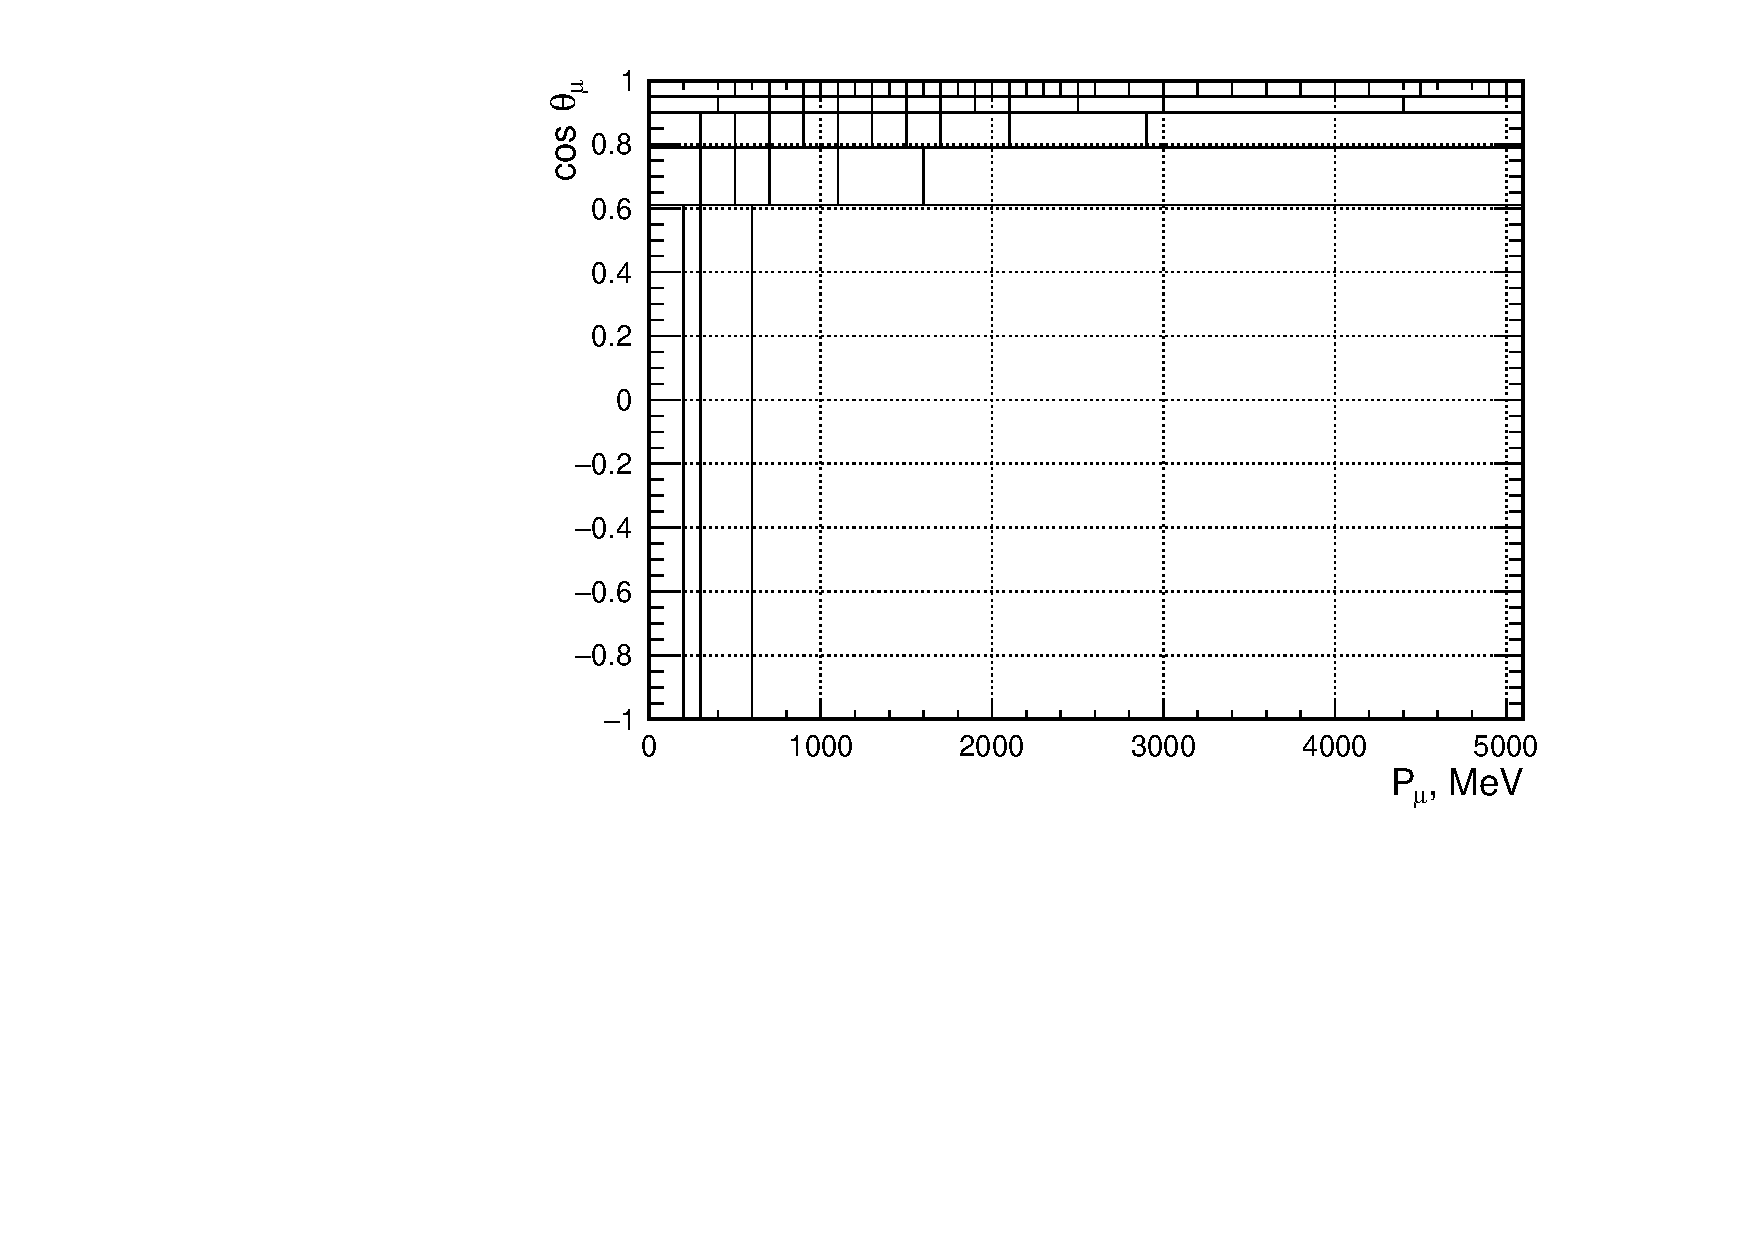
\includegraphics[width=0.95\linewidth]{figs/TH2PolyReset5000_MC_FGD2_anti-numuCC_other}
  \caption{FGD2 RHC $\bar{\nu_{\mu}}$ Other}
  \label{fig:TH2Poly_Reset5000FGD2_anti-numuCC_other}
\end{subfigure}
\begin{subfigure}{.32\textwidth}
  \centering
  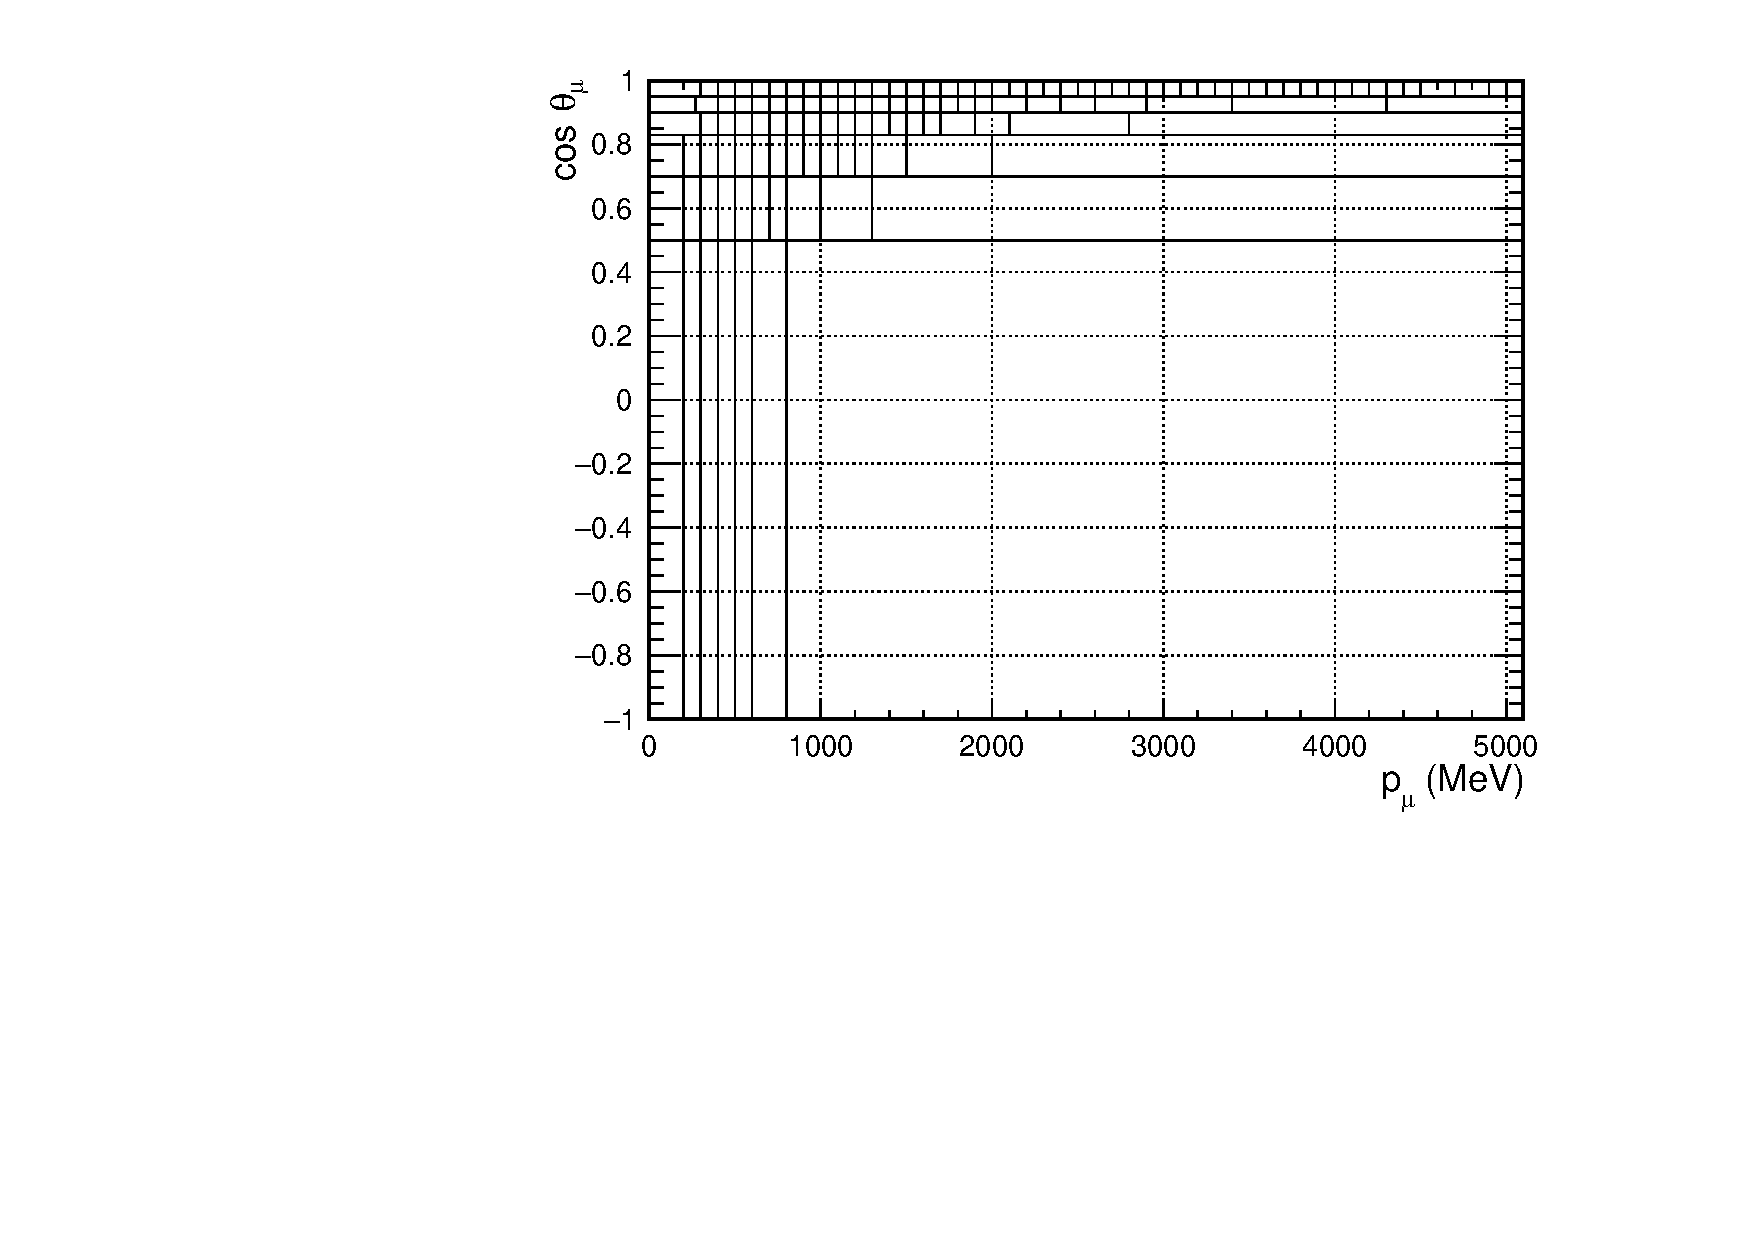
\includegraphics[width=0.95\linewidth]{figs/TH2PolyReset5000_MC_FGD1_NuMuBkg_CC0pi_in_AntiNu_Mode}
  \caption{FGD1 RHC $\nu_{\mu}$ 0$\pi$}
  \label{fig:TH2Poly_Reset5000FGD1_NuMuBkg_CC0pi_in_AntiNu_Mode}
\end{subfigure}
\begin{subfigure}{.32\textwidth}
  \centering
  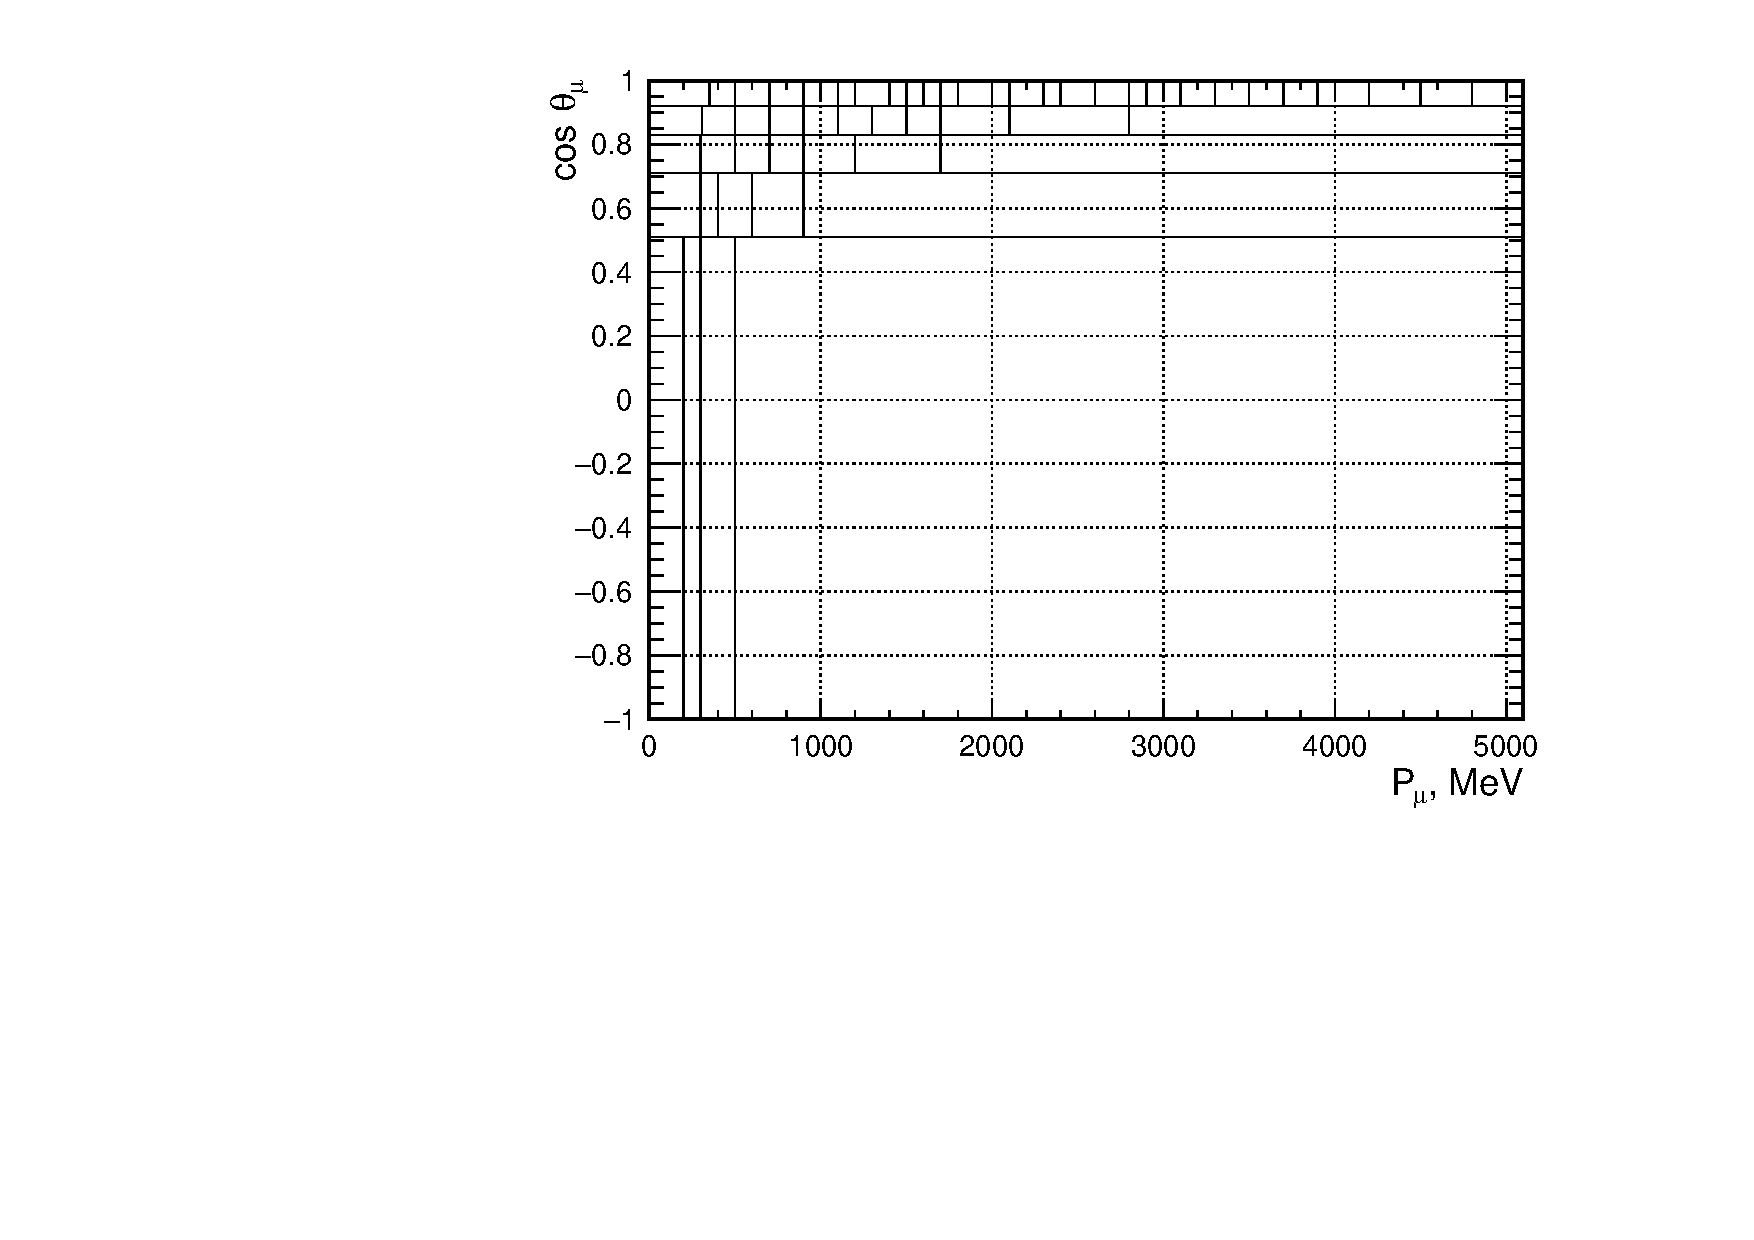
\includegraphics[width=0.95\linewidth]{figs/TH2PolyReset5000_MC_FGD1_NuMuBkg_CC1pi_in_AntiNu_Mode}
  \caption{FGD1 RHC $\nu_{\mu}$ 1$\pi$}
  \label{fig:TH2Poly_Reset5000FGD1_NuMuBkg_CC1pi_in_AntiNu_Mode}
\end{subfigure}
\begin{subfigure}{.32\textwidth}
  \centering
  \includegraphics[width=0.95\linewidth]{figs/TH2PolyReset5000_MC_FGD1_NuMuBkg_CCOther_in_AntiNu_Mode}
  \caption{FGD1 RHC $\nu_{\mu}$ Other}
  \label{fig:TH2Poly_Reset5000FGD1_NuMuBkg_CCOther_in_AntiNu_Mode}
\end{subfigure}
\begin{subfigure}{.32\textwidth}
  \centering
  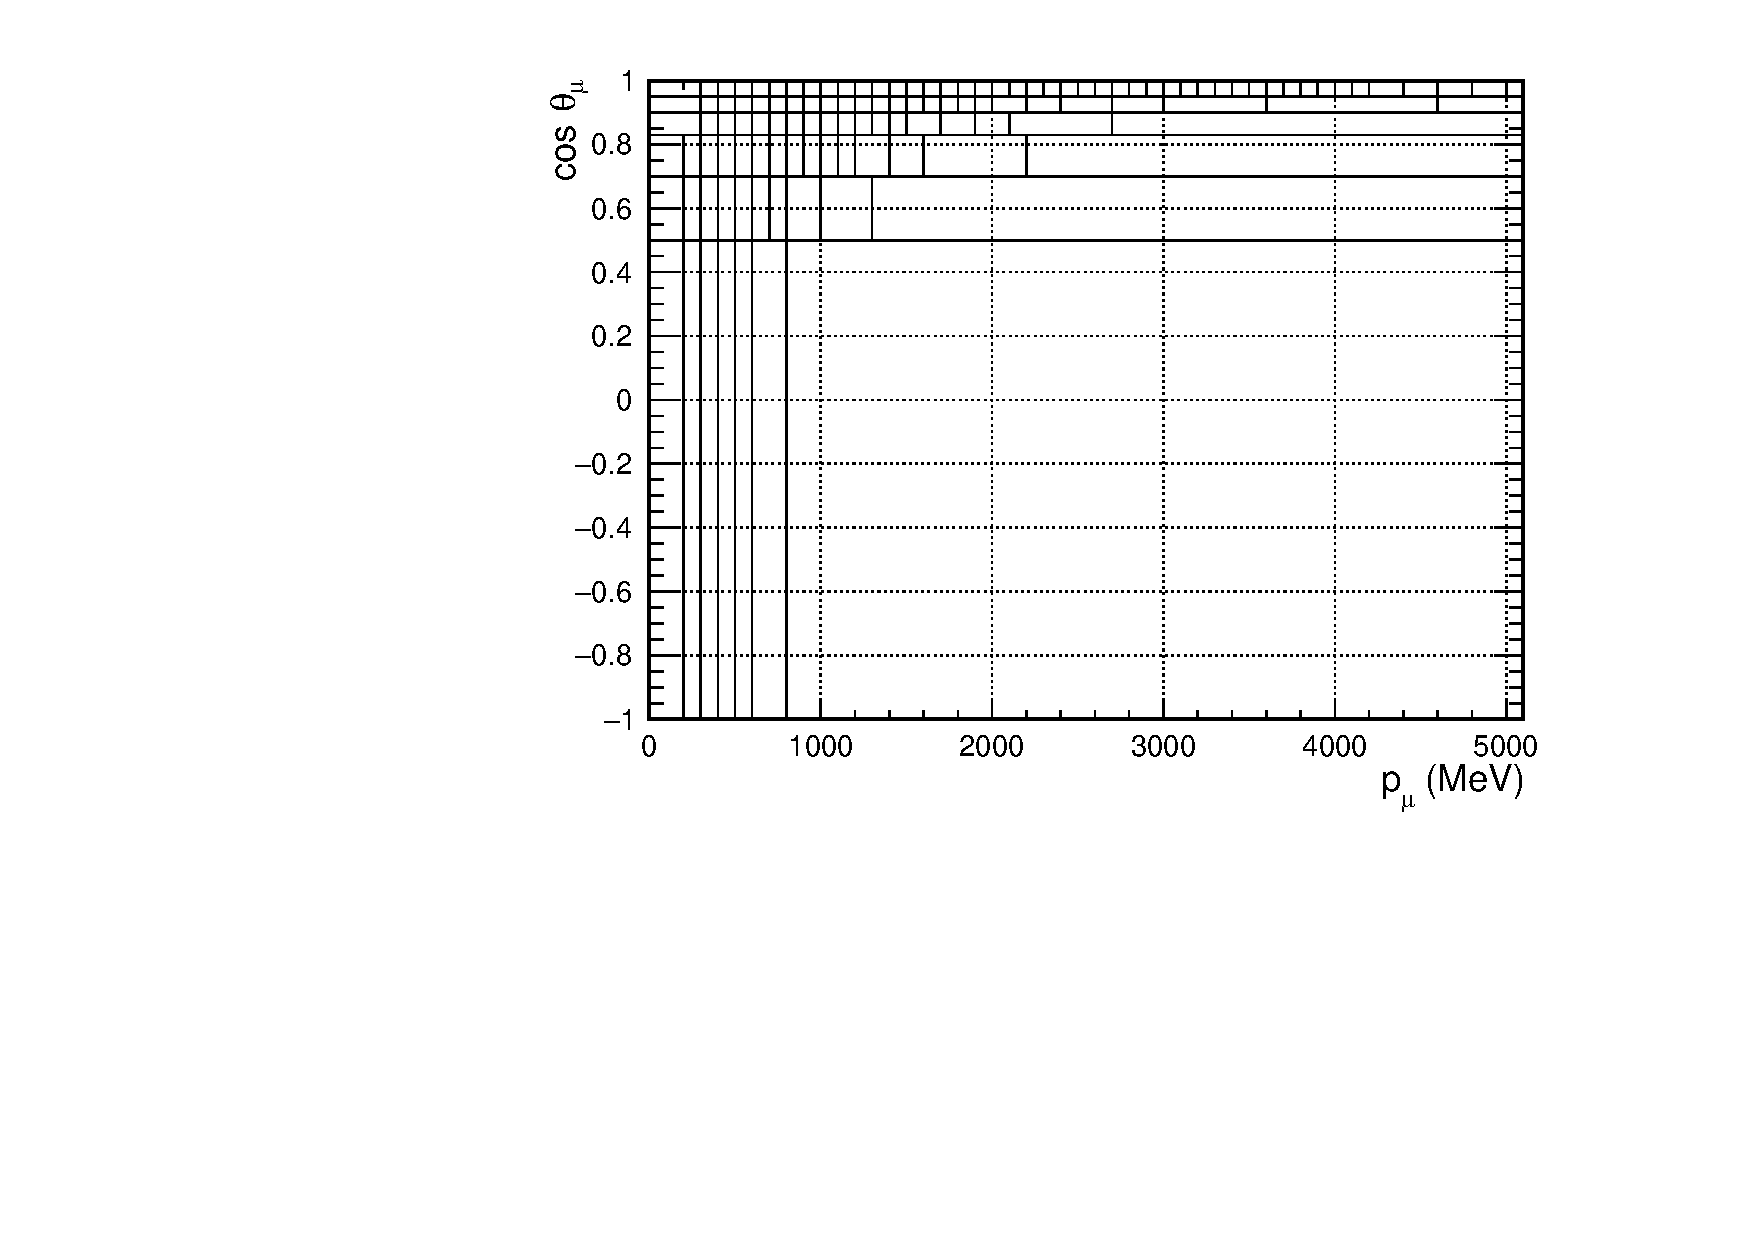
\includegraphics[width=0.95\linewidth]{figs/TH2PolyReset5000_MC_FGD2_NuMuBkg_CC0pi_in_AntiNu_Mode}
  \caption{FGD2 RHC $\nu_{\mu}$ 0$\pi$}
  \label{fig:TH2Poly_Reset5000FGD2_NuMuBkg_CC0pi_in_AntiNu_Mode}
\end{subfigure}
\begin{subfigure}{.32\textwidth}
  \centering
  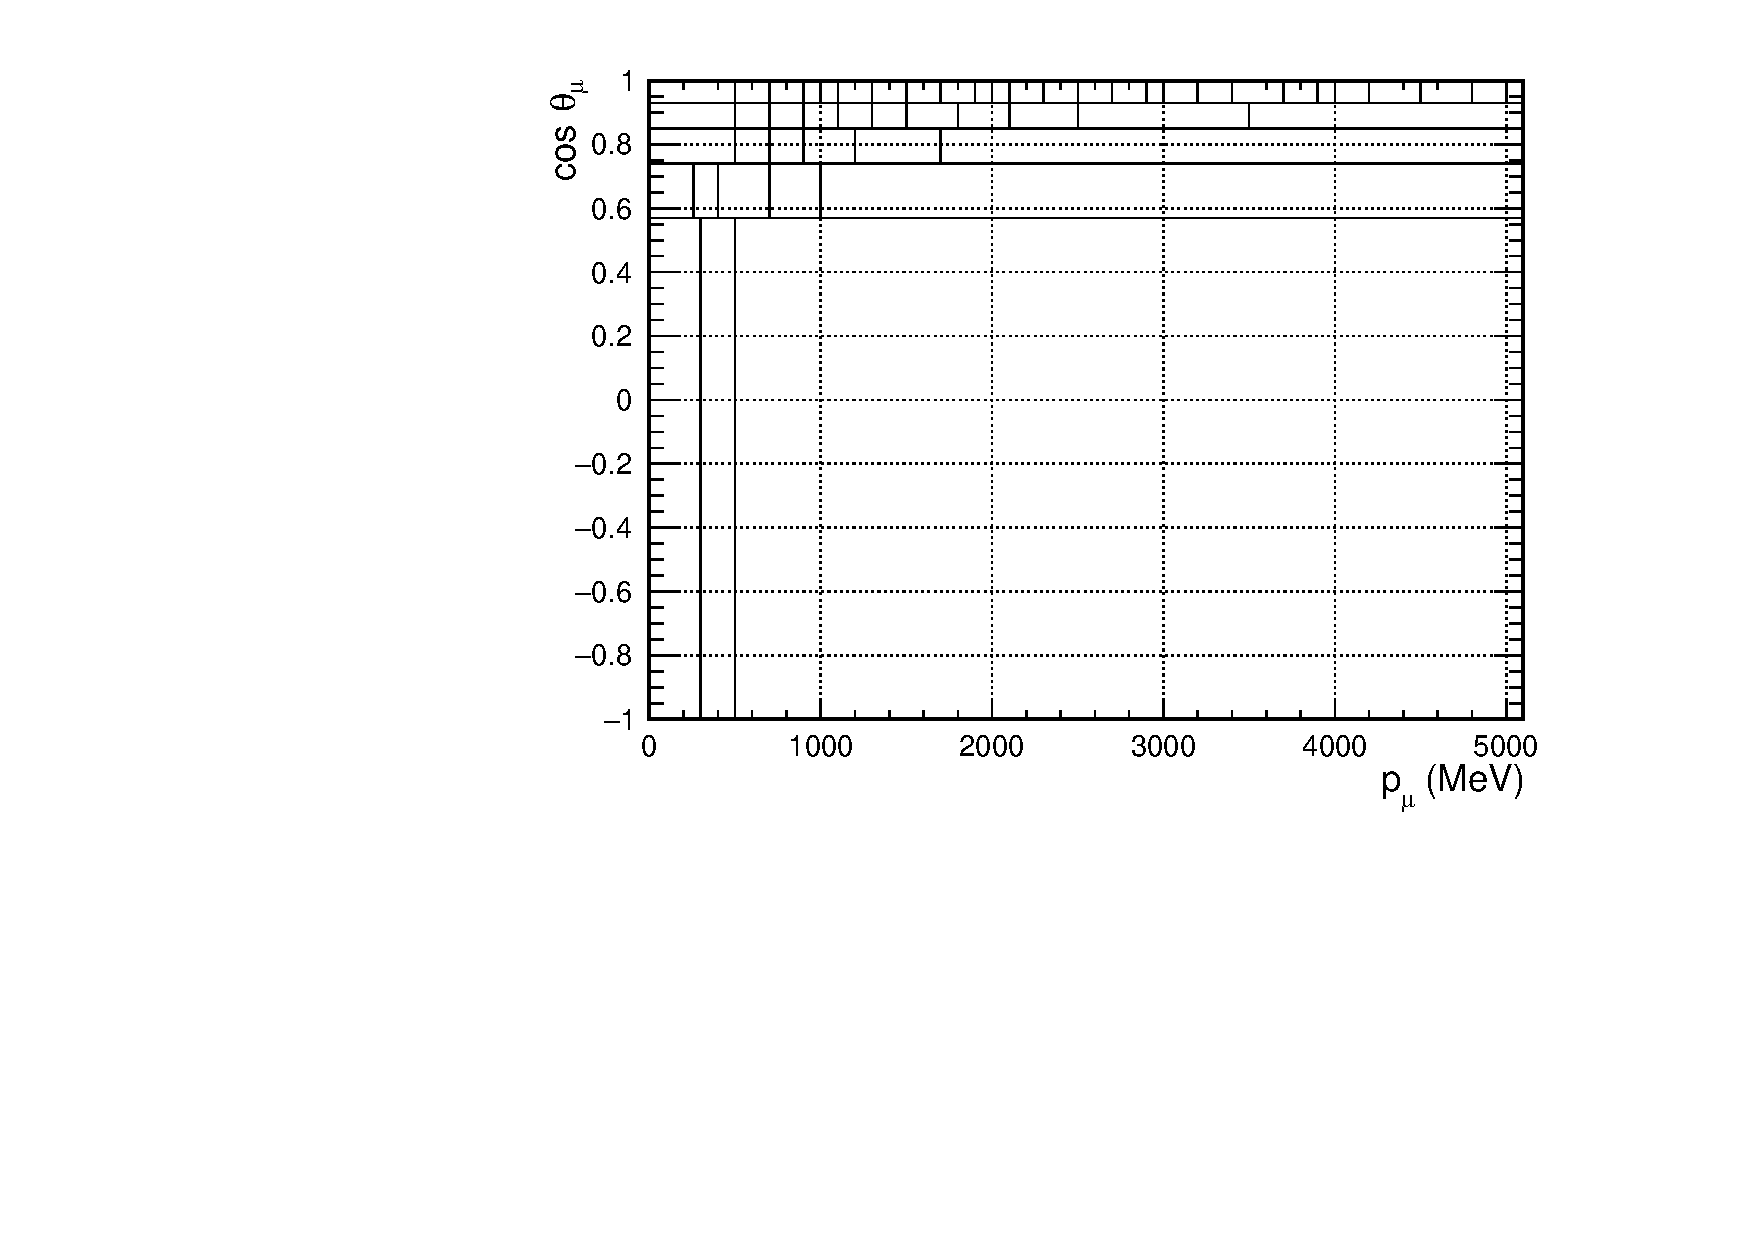
\includegraphics[width=0.95\linewidth]{figs/TH2PolyReset5000_MC_FGD2_NuMuBkg_CC1pi_in_AntiNu_Mode}
  \caption{FGD2 RHC $\nu_{\mu}$ 1$\pi$}
  \label{fig:TH2Poly_Reset5000FGD2_NuMuBkg_CC1pi_in_AntiNu_Mode}
\end{subfigure}
\begin{subfigure}{.32\textwidth}
  \centering
  \includegraphics[width=0.95\linewidth]{figs/TH2PolyReset5000_MC_FGD2_NuMuBkg_CCOther_in_AntiNu_Mode}
  \caption{FGD2 RHC $\nu_{\mu}$ Other}
  \label{fig:TH2Poly_Reset5000FGD2_NuMuBkg_CCOther_in_AntiNu_Mode}
\end{subfigure}
\caption{Non-uniform rectangular binning used in this analysis for each sample. The x-axis is reduced to better show the smaller bins at low momentum and high angle.}
\label{fig:th2polybinreset5000}
\end{figure}

\begin{figure}
\centering
\begin{subfigure}{.32\textwidth}
  \centering
  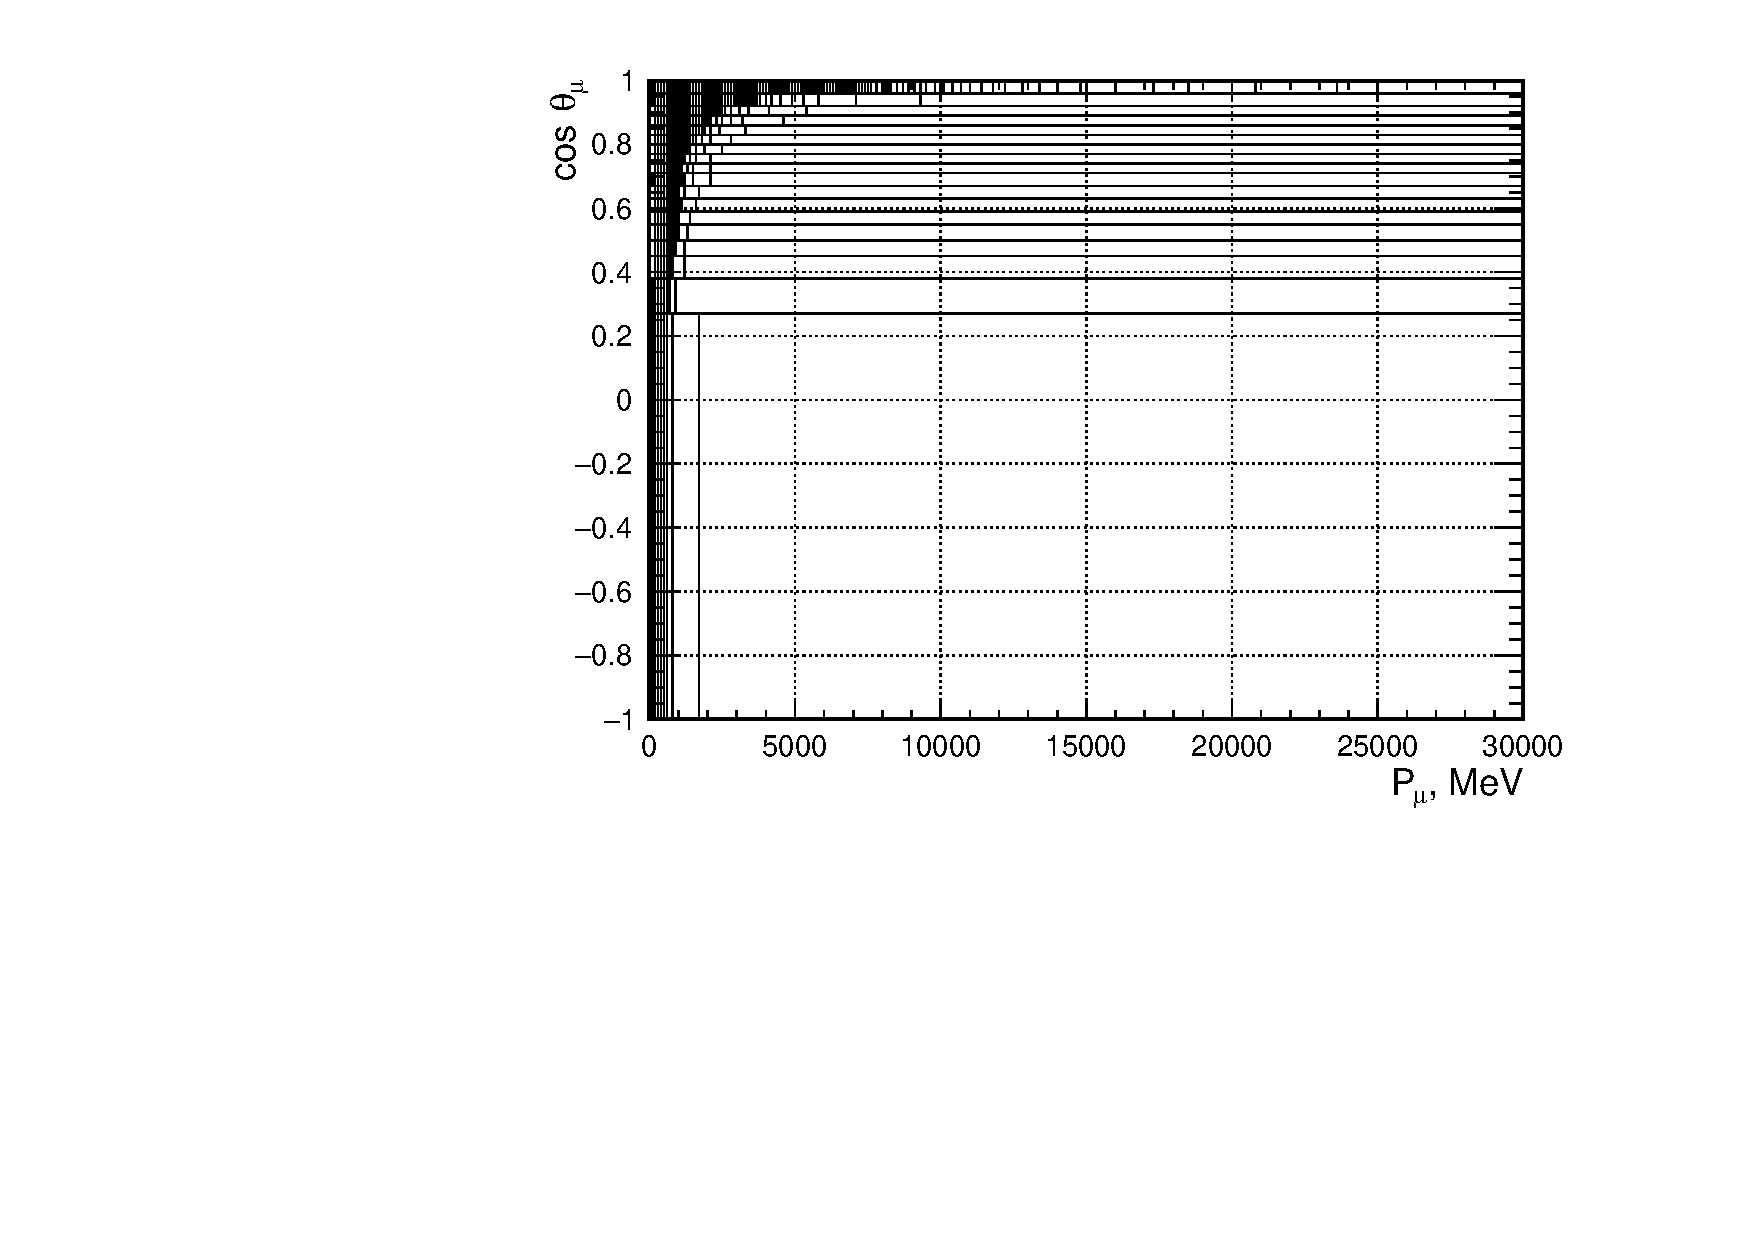
\includegraphics[width=0.95\linewidth]{figs/TH2PolyReset_MC_FGD1_numuCC_0pi}
  \caption{FGD1 FHC $\nu_{\mu}$ 0$\pi$}
  \label{fig:TH2Poly_ResetFGD1_numuCC_0pi}
\end{subfigure}
\begin{subfigure}{.32\textwidth}
  \centering
  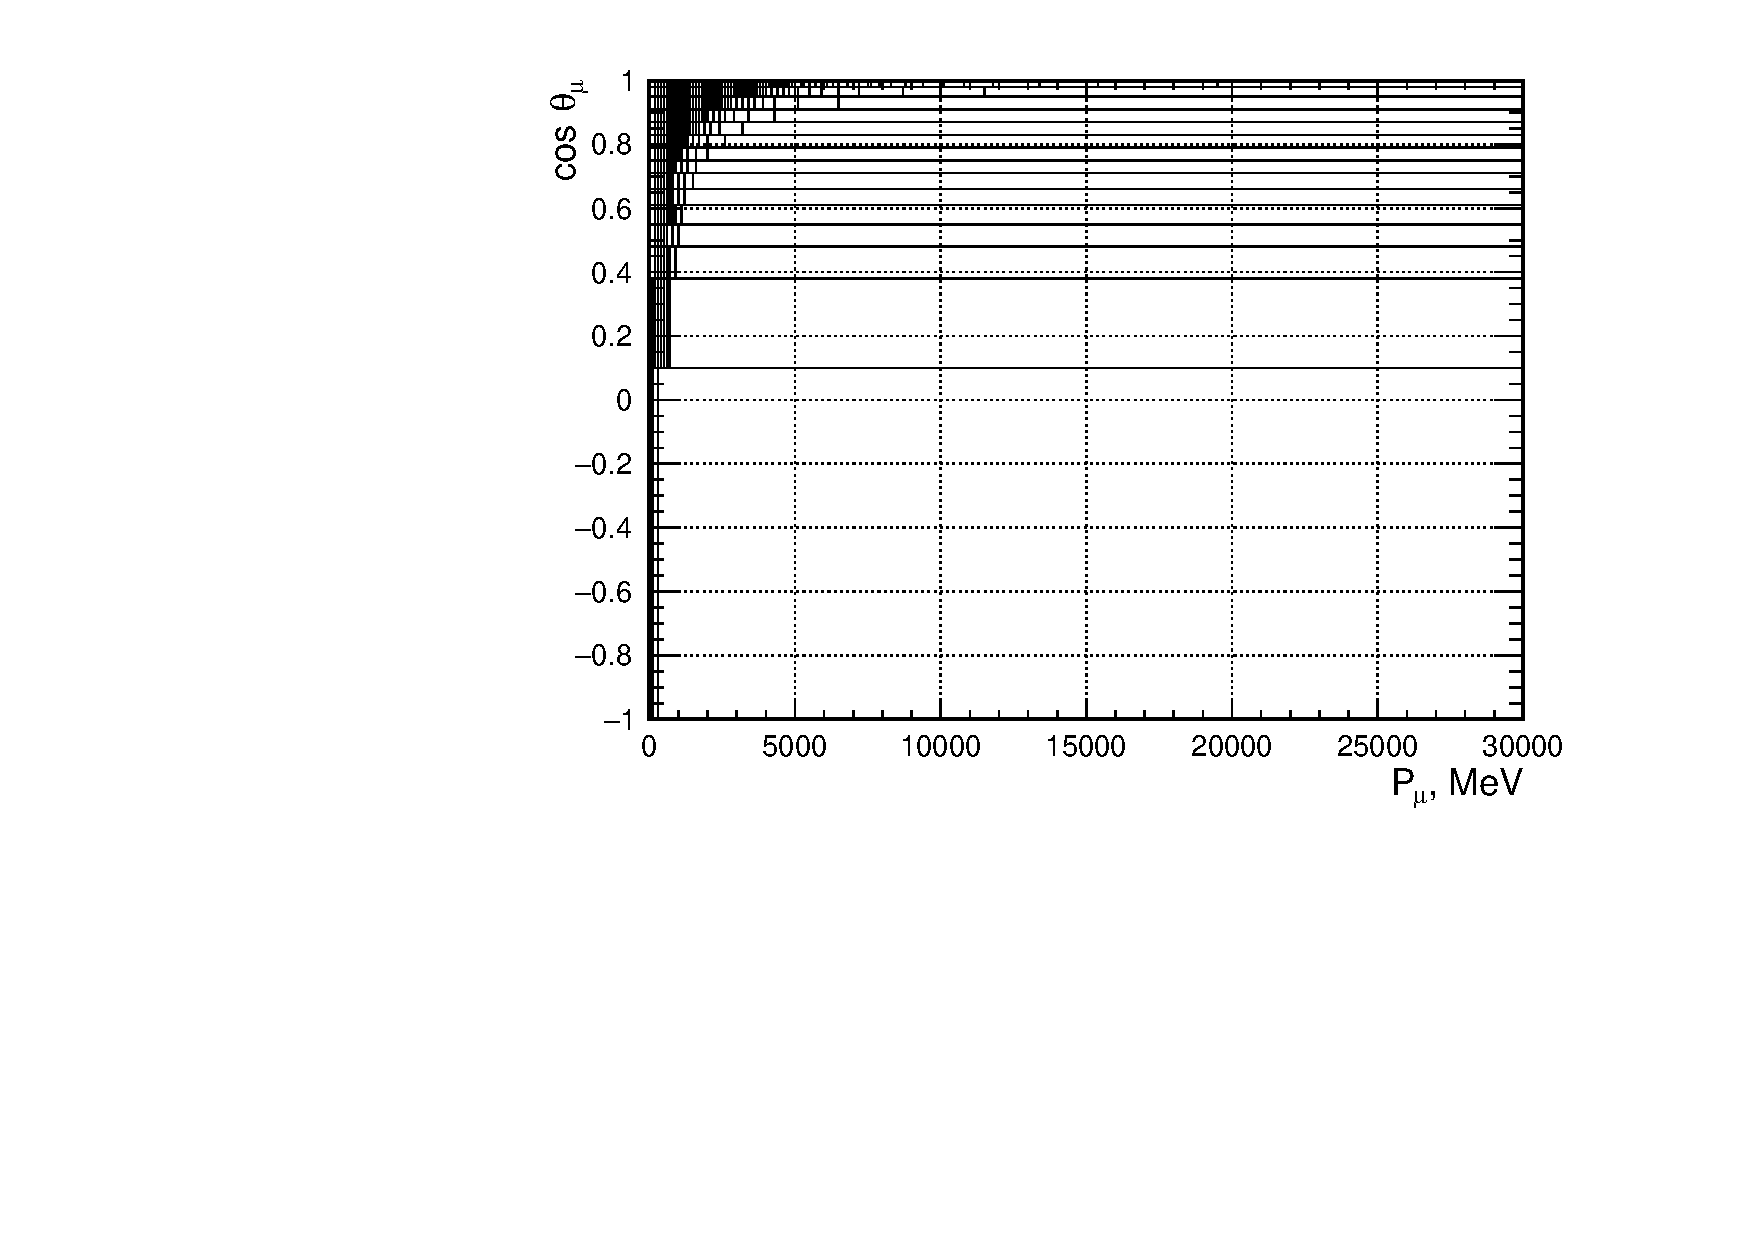
\includegraphics[width=0.95\linewidth]{figs/TH2PolyReset_MC_FGD1_numuCC_1pi}
  \caption{FGD1 FHC $\nu_{\mu}$ 1$\pi$}
  \label{fig:TH2Poly_ResetFGD1_numuCC_1pi}
\end{subfigure}
\begin{subfigure}{.32\textwidth}
  \centering
  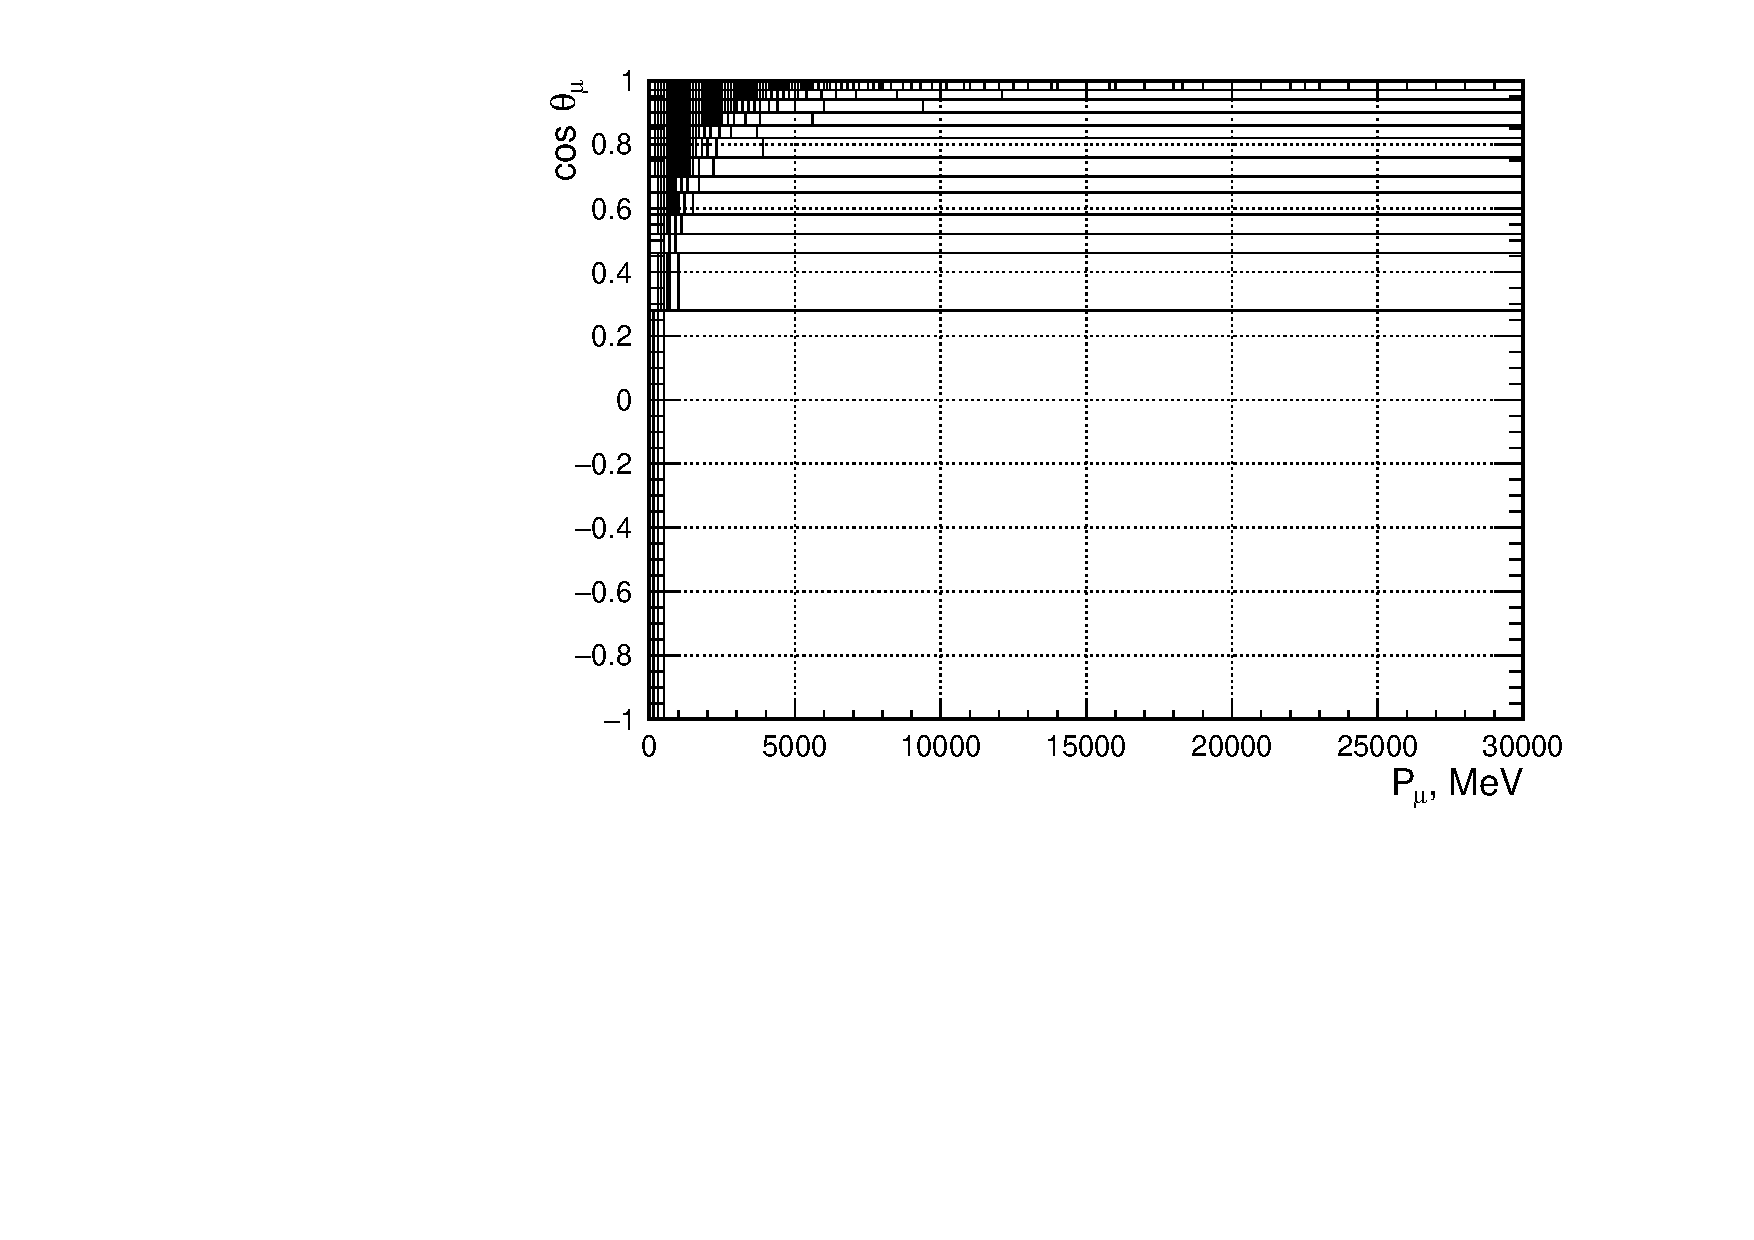
\includegraphics[width=0.95\linewidth]{figs/TH2PolyReset_MC_FGD1_numuCC_other}
  \caption{FGD1 FHC $\nu_{\mu}$ Other}
  \label{fig:TH2Poly_ResetFGD1_numuCC_other}
\end{subfigure}
\centering
\begin{subfigure}{.32\textwidth}
  \centering
  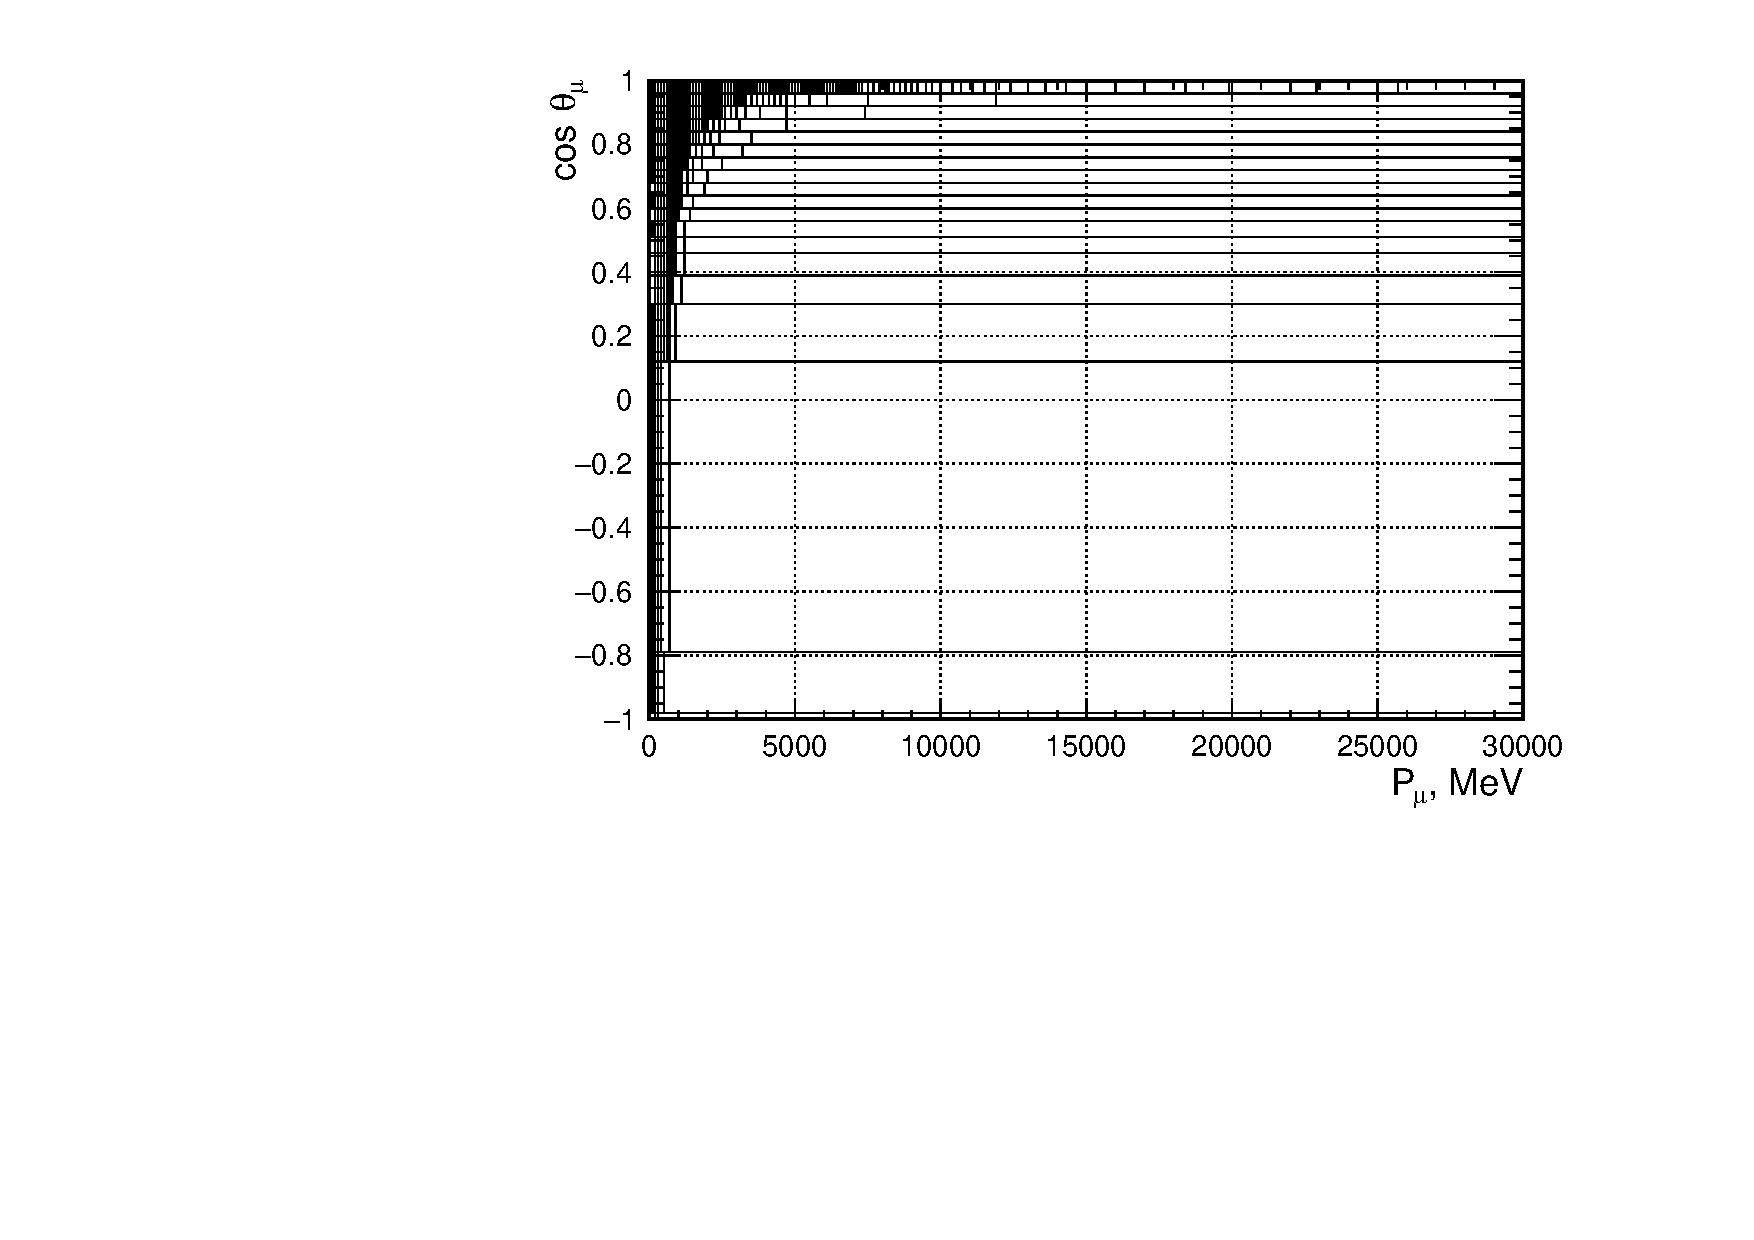
\includegraphics[width=0.95\linewidth]{figs/TH2PolyReset_MC_FGD2_numuCC_0pi}
  \caption{FGD2 FHC $\nu_{\mu}$ 0$\pi$}
  \label{fig:TH2Poly_ResetFGD2_numuCC_0pi}
\end{subfigure}
\begin{subfigure}{.32\textwidth}
  \centering
  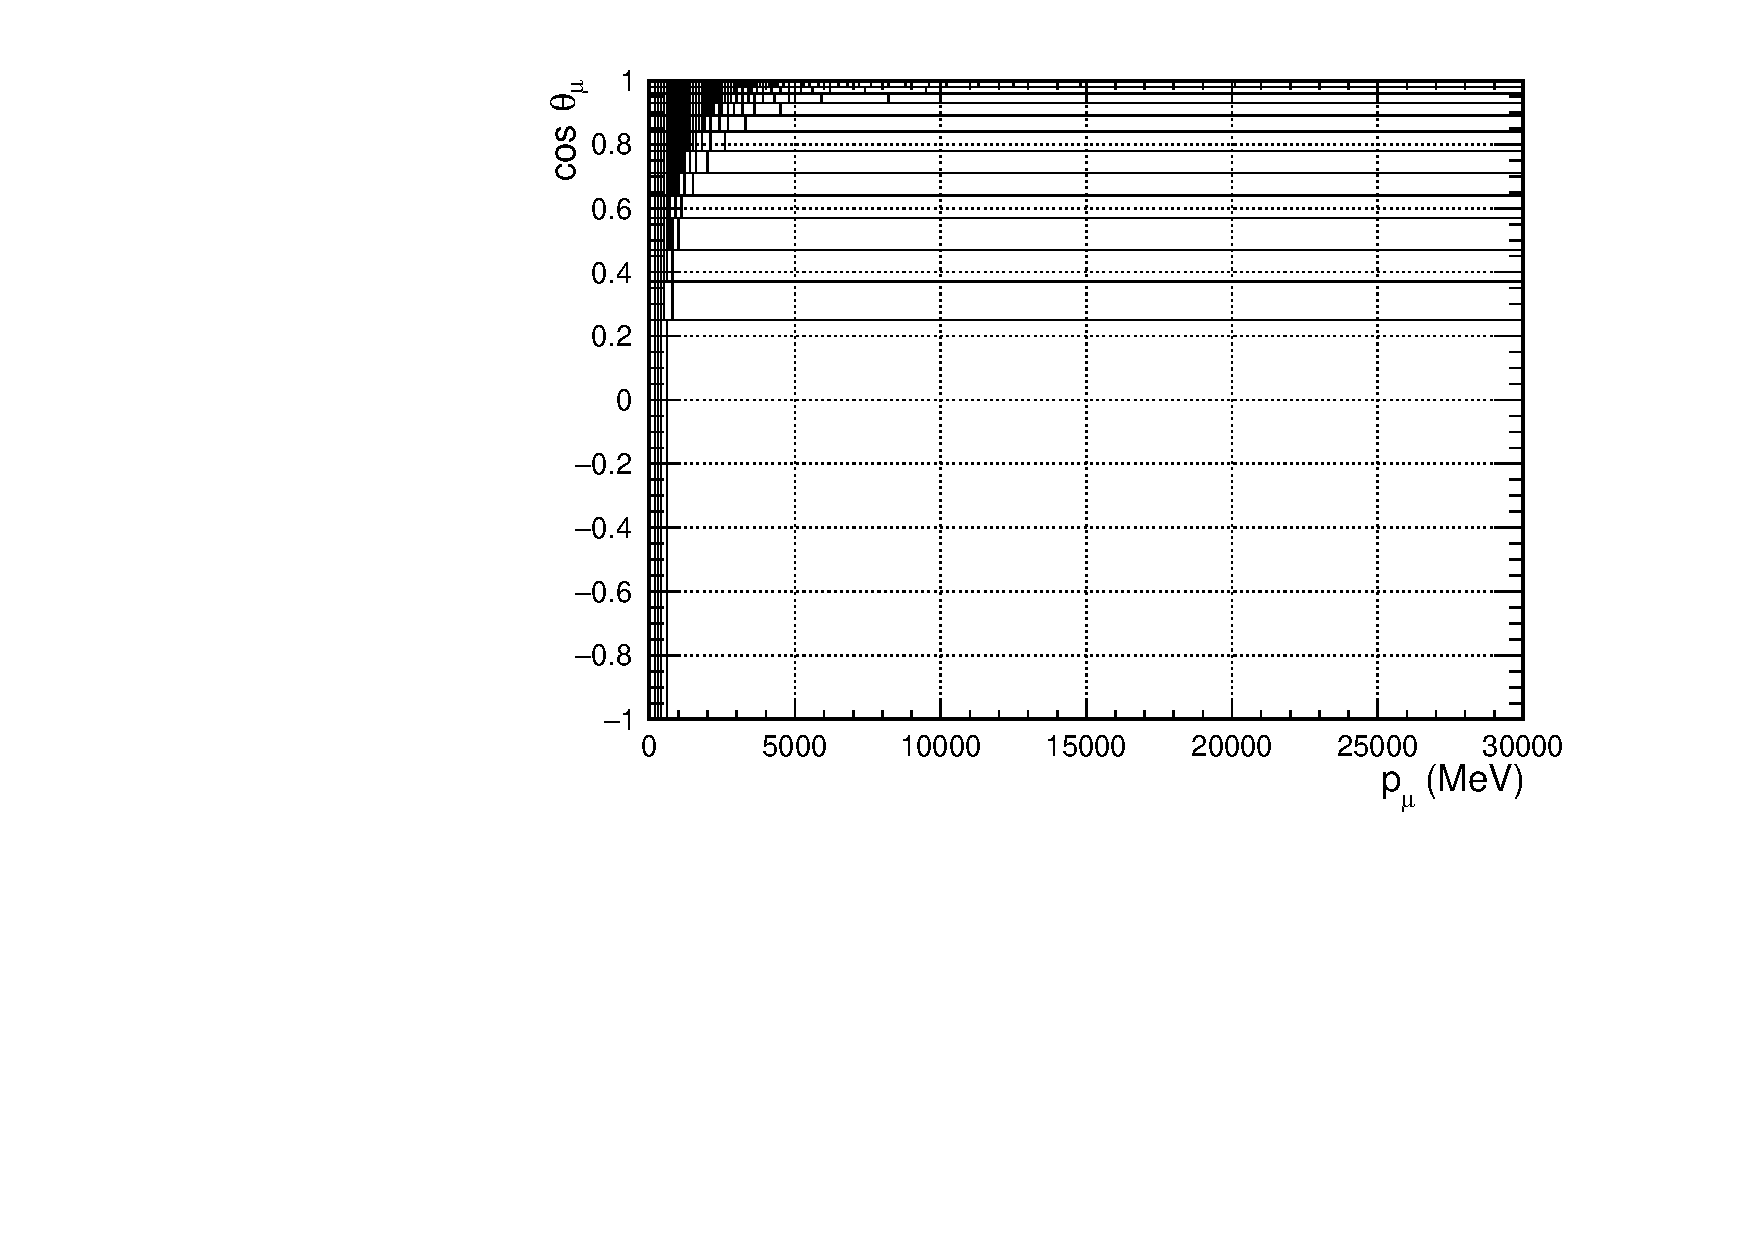
\includegraphics[width=0.95\linewidth]{figs/TH2PolyReset_MC_FGD2_numuCC_1pi}
  \caption{FGD2 FHC $\nu_{\mu}$ 1$\pi$}
  \label{fig:TH2Poly_ResetFGD2_numuCC_1pi}
\end{subfigure}
\begin{subfigure}{.32\textwidth}
  \centering
  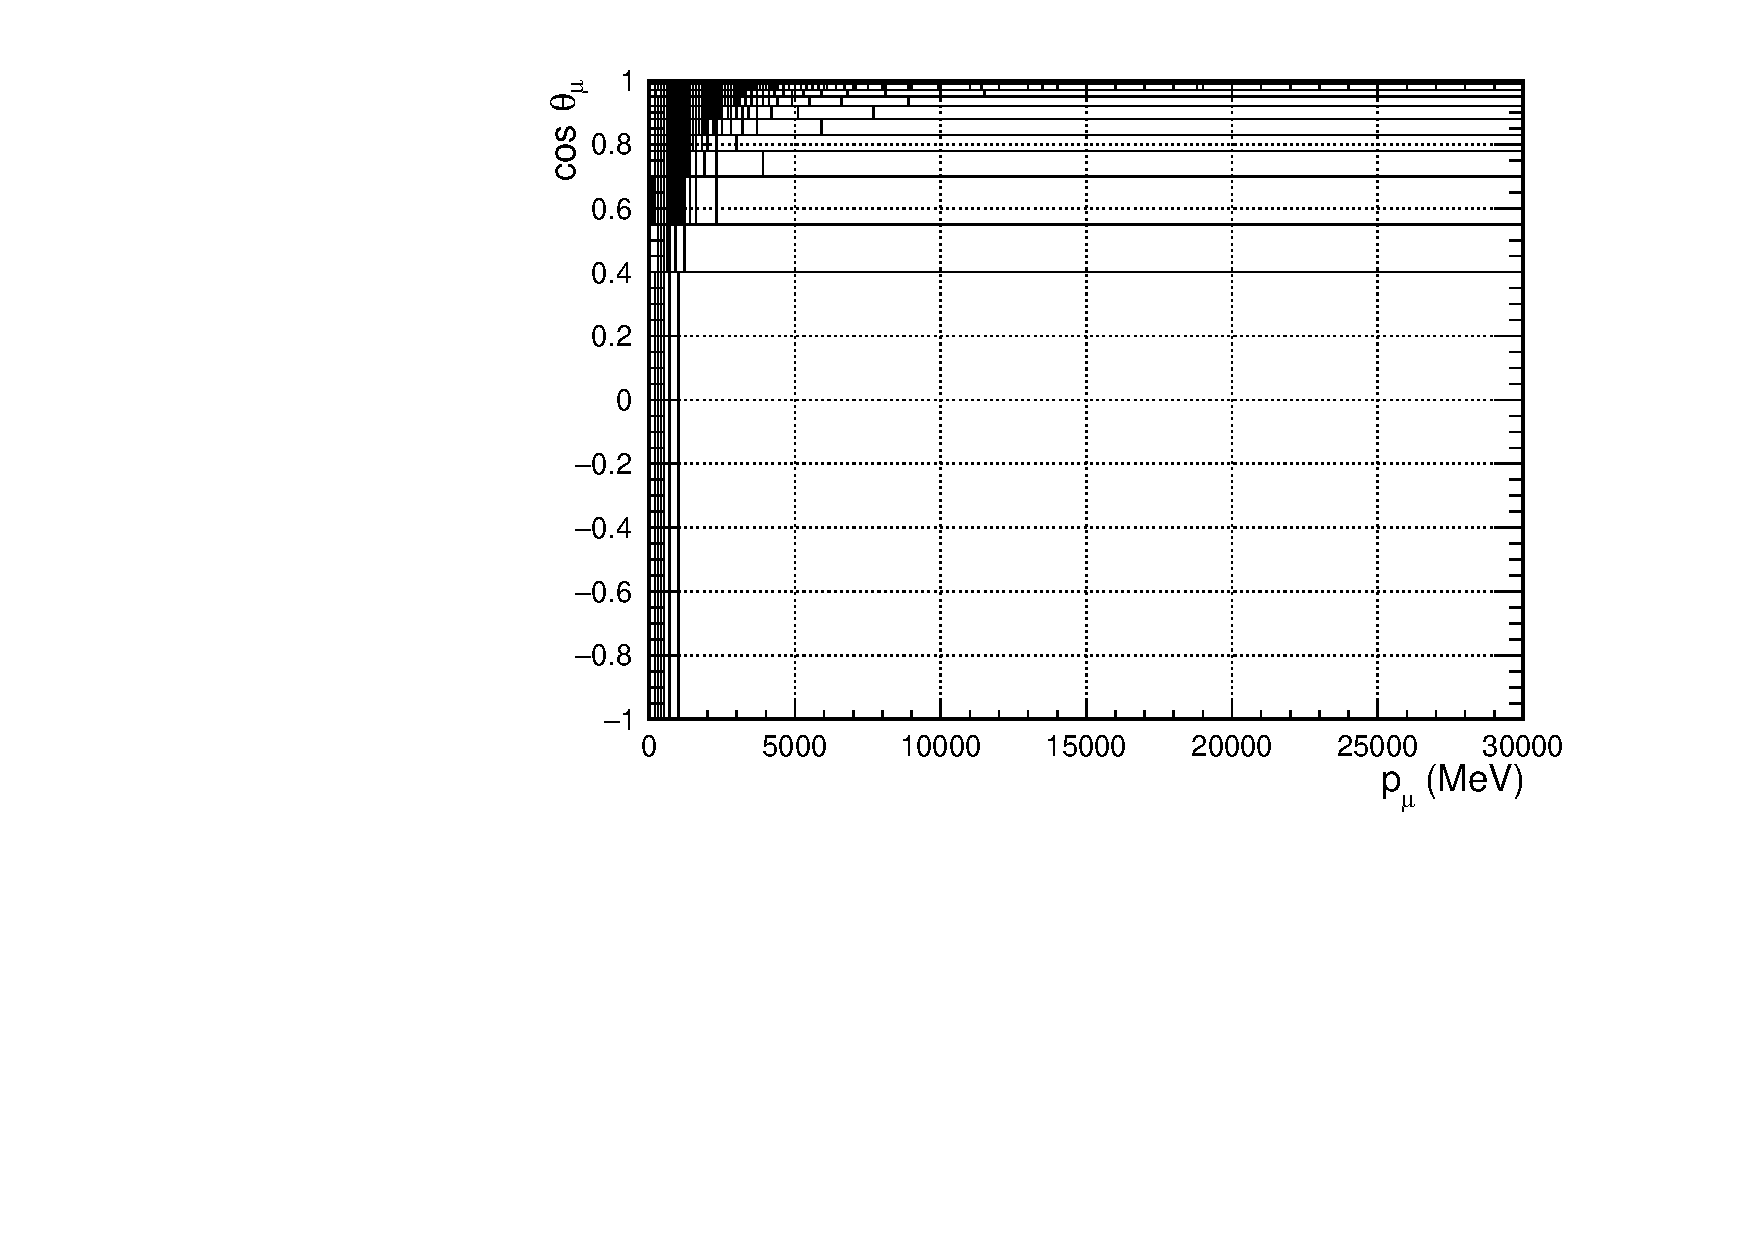
\includegraphics[width=0.95\linewidth]{figs/TH2PolyReset_MC_FGD2_numuCC_other}
  \caption{FGD2 FHC $\nu_{\mu}$ Other}
  \label{fig:TH2Poly_ResetFGD2_numuCC_other}
\end{subfigure}
\centering
\begin{subfigure}{.32\textwidth}
  \centering
  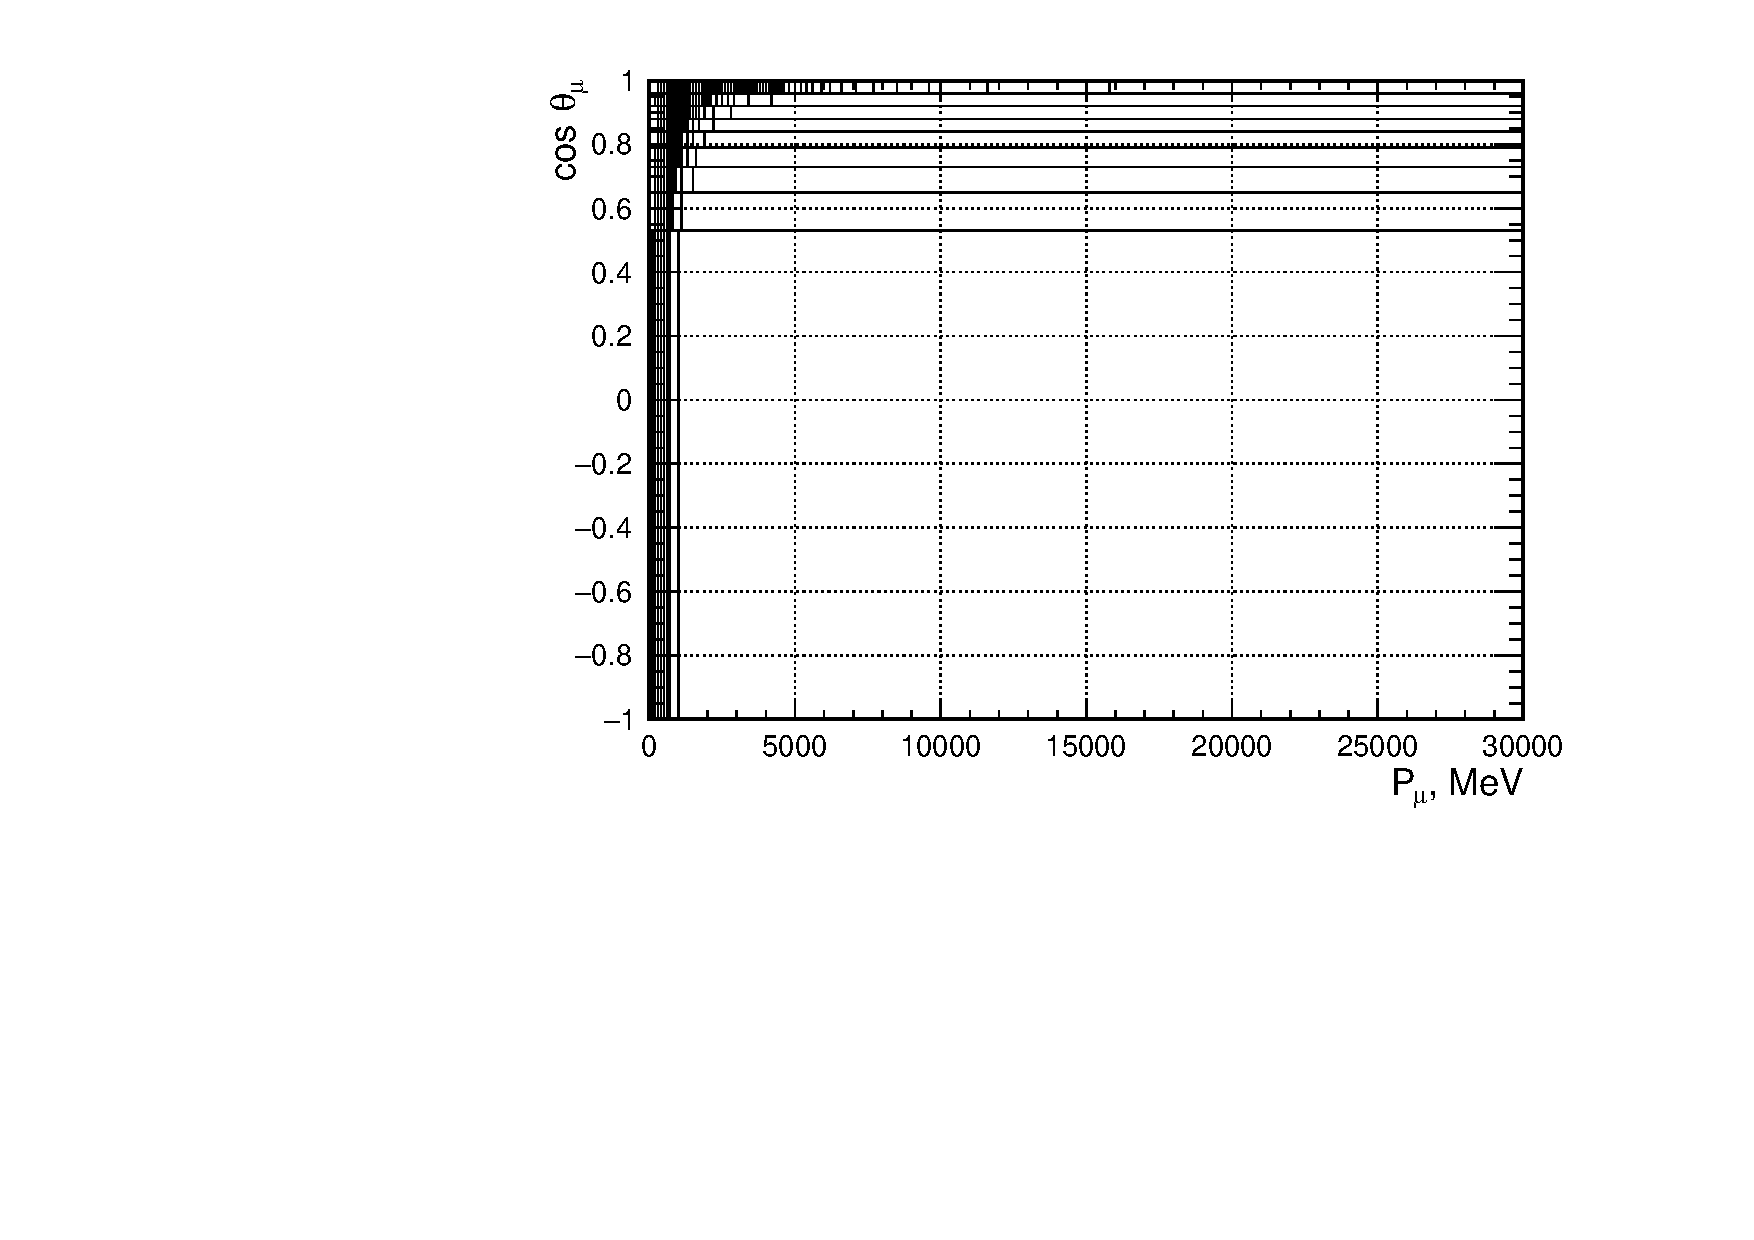
\includegraphics[width=0.95\linewidth]{figs/TH2PolyReset_MC_FGD1_anti-numuCC_0pi}
  \caption{FGD1 RHC $\bar{\nu_{\mu}}$ 0$\pi$}
  \label{fig:TH2Poly_ResetFGD1_anti-numuCC_0pi}
\end{subfigure}
\begin{subfigure}{.32\textwidth}
  \centering
  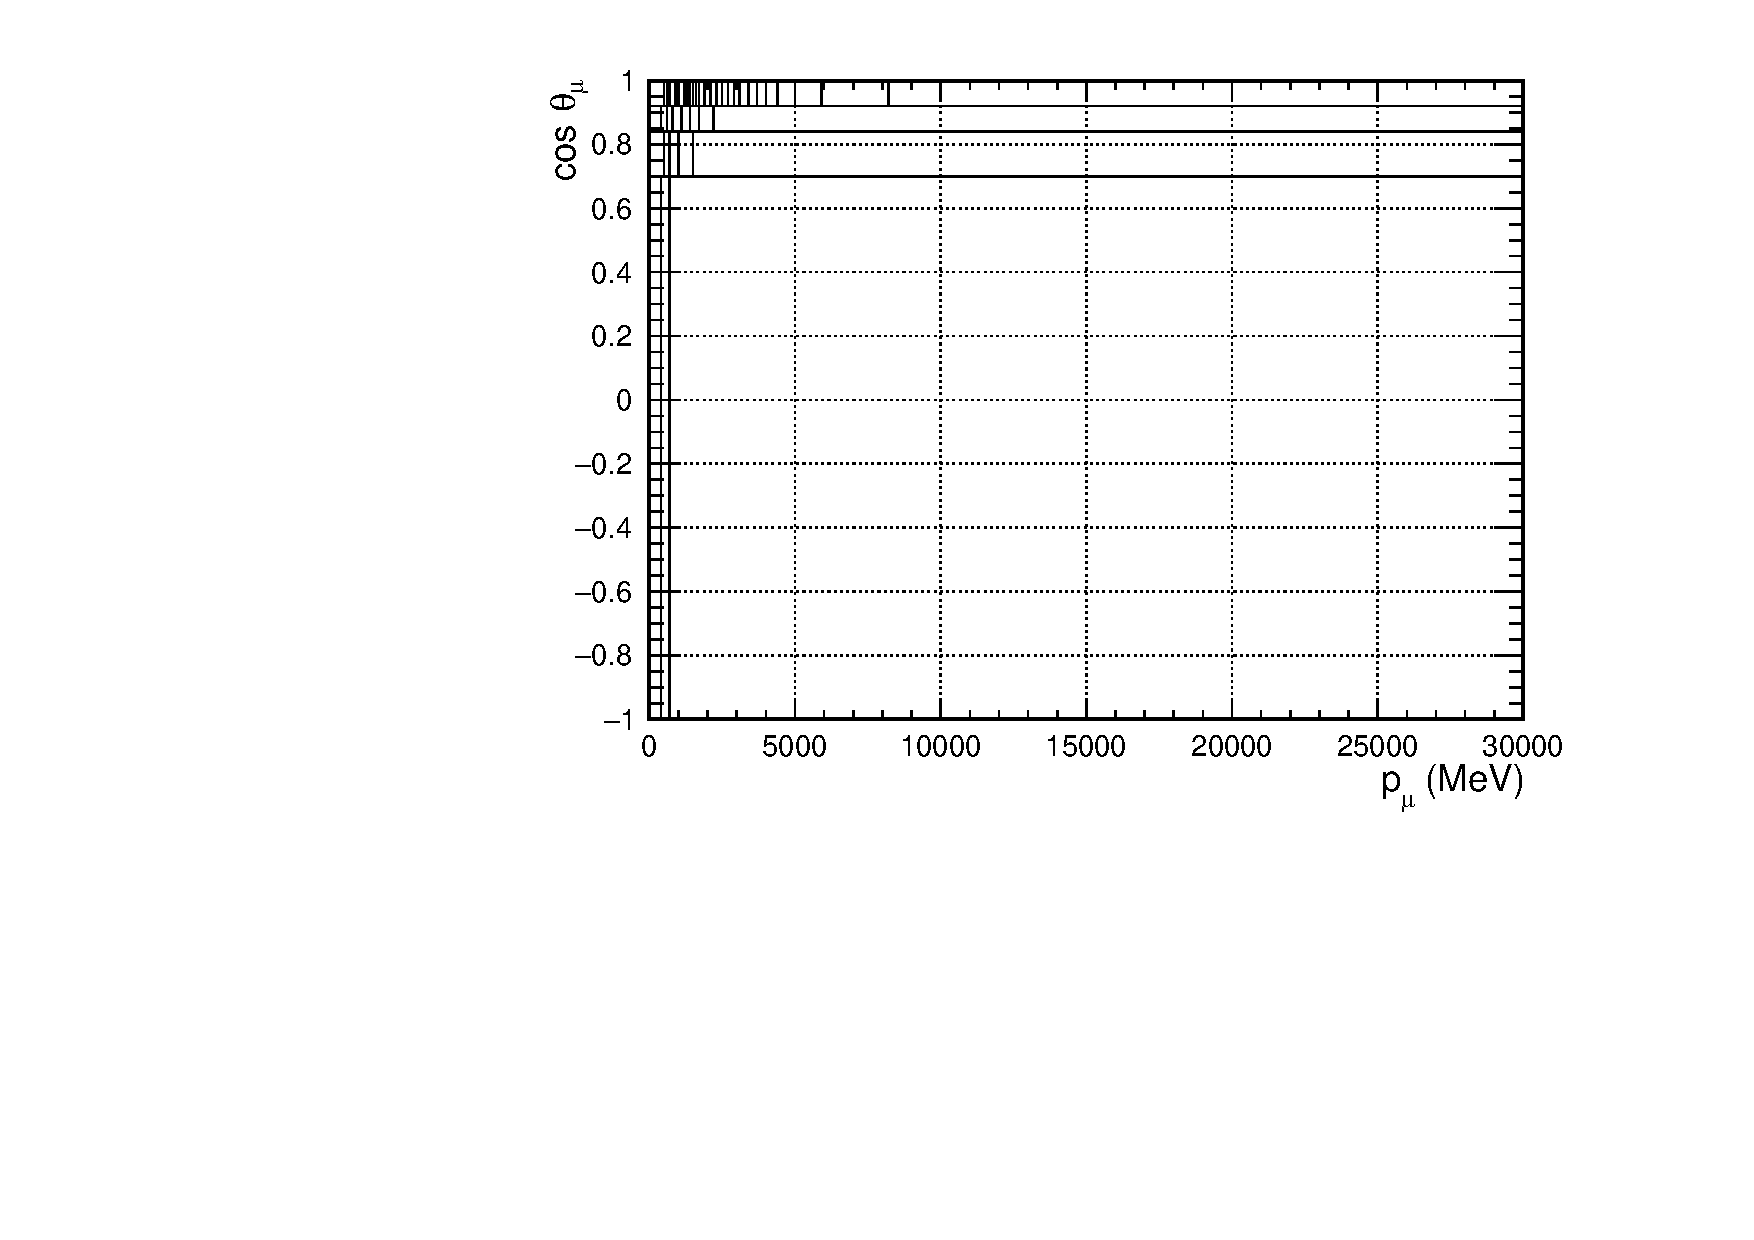
\includegraphics[width=0.95\linewidth]{figs/TH2PolyReset_MC_FGD1_anti-numuCC_1pi}
  \caption{FGD1 RHC $\bar{\nu_{\mu}}$ 1$\pi$}
  \label{fig:th2polyTH2Poly_ResetFGD1_anti-numuCC_1pi}
\end{subfigure}
\begin{subfigure}{.32\textwidth}
  \centering
  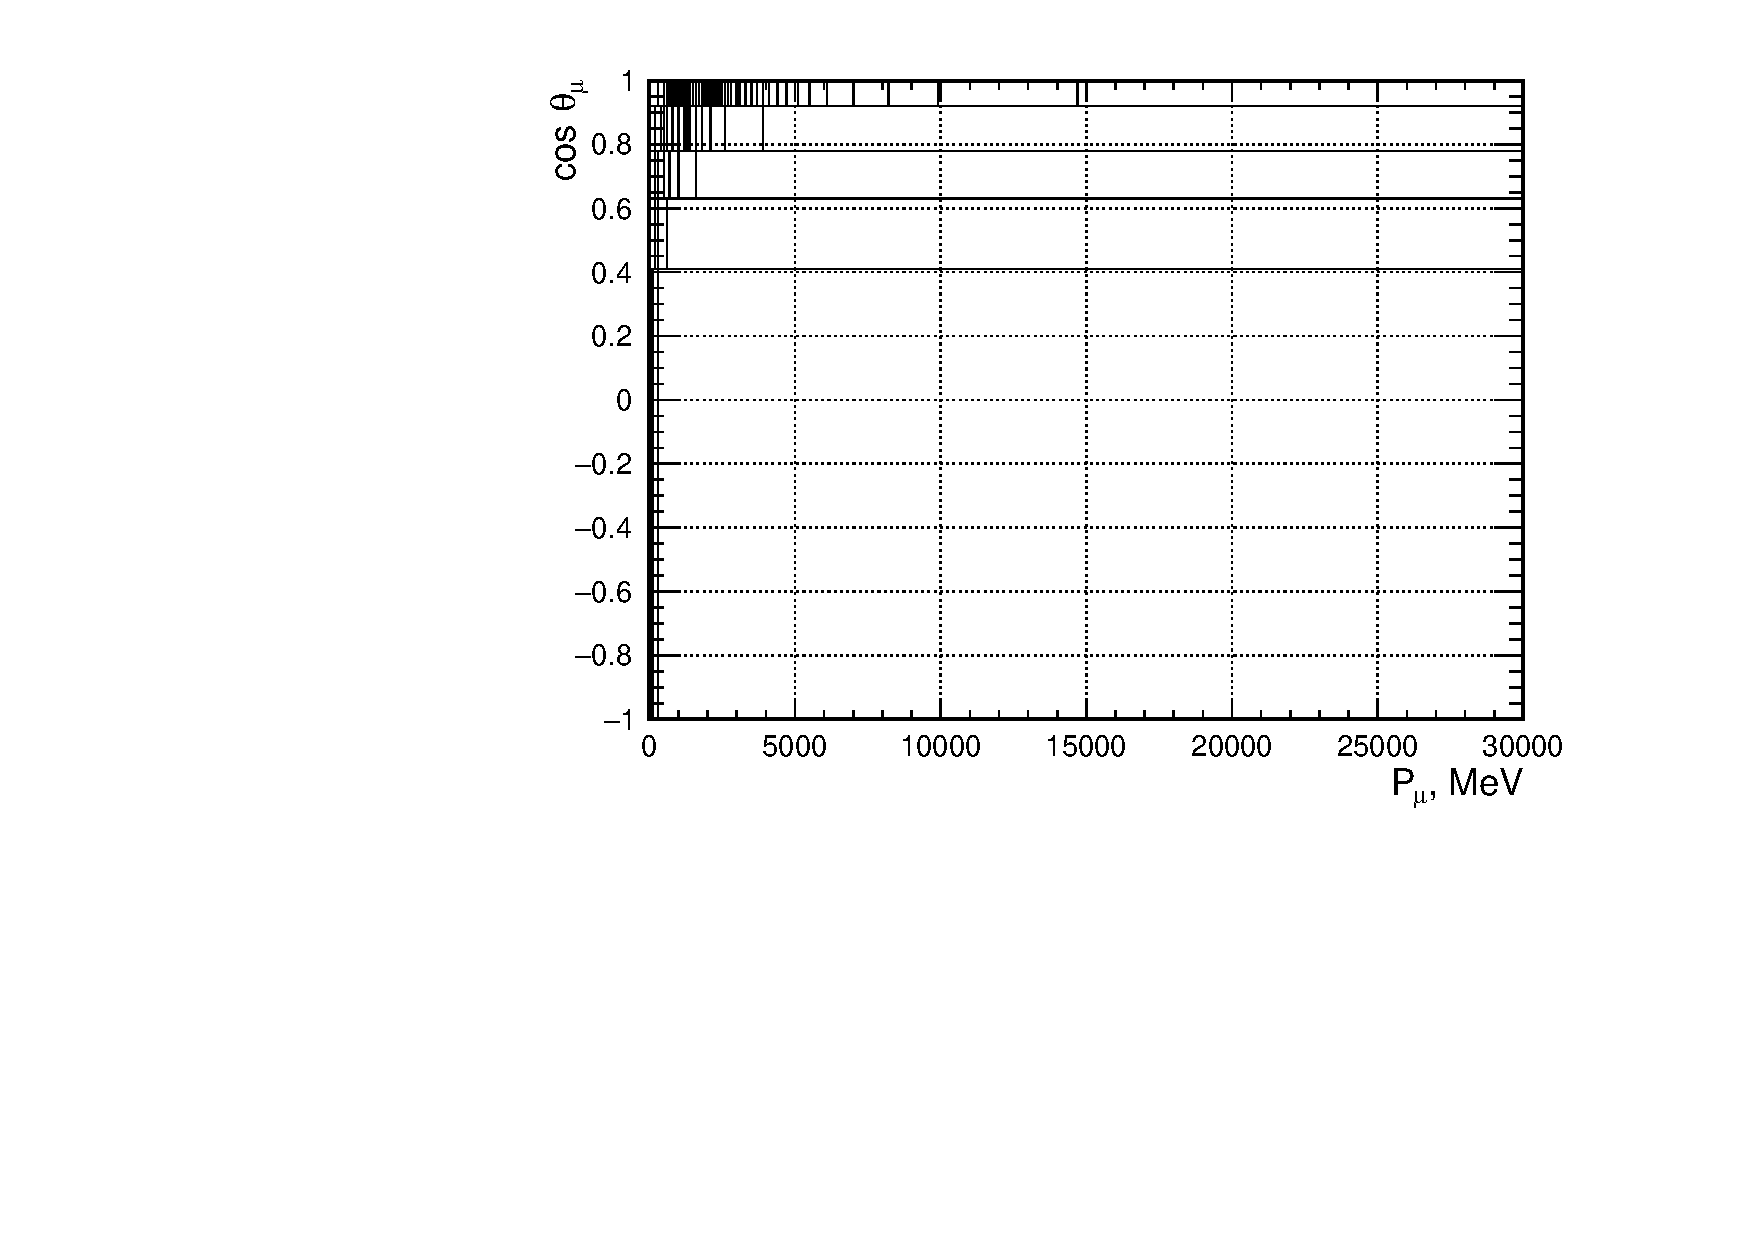
\includegraphics[width=0.95\linewidth]{figs/TH2PolyReset_MC_FGD1_anti-numuCC_other}
  \caption{FGD1 RHC $\bar{\nu_{\mu}}$ Other}
  \label{fig:TH2Poly_ResetFGD1_anti-numuCC_other}
\end{subfigure}
\centering
\begin{subfigure}{.32\textwidth}
  \centering
  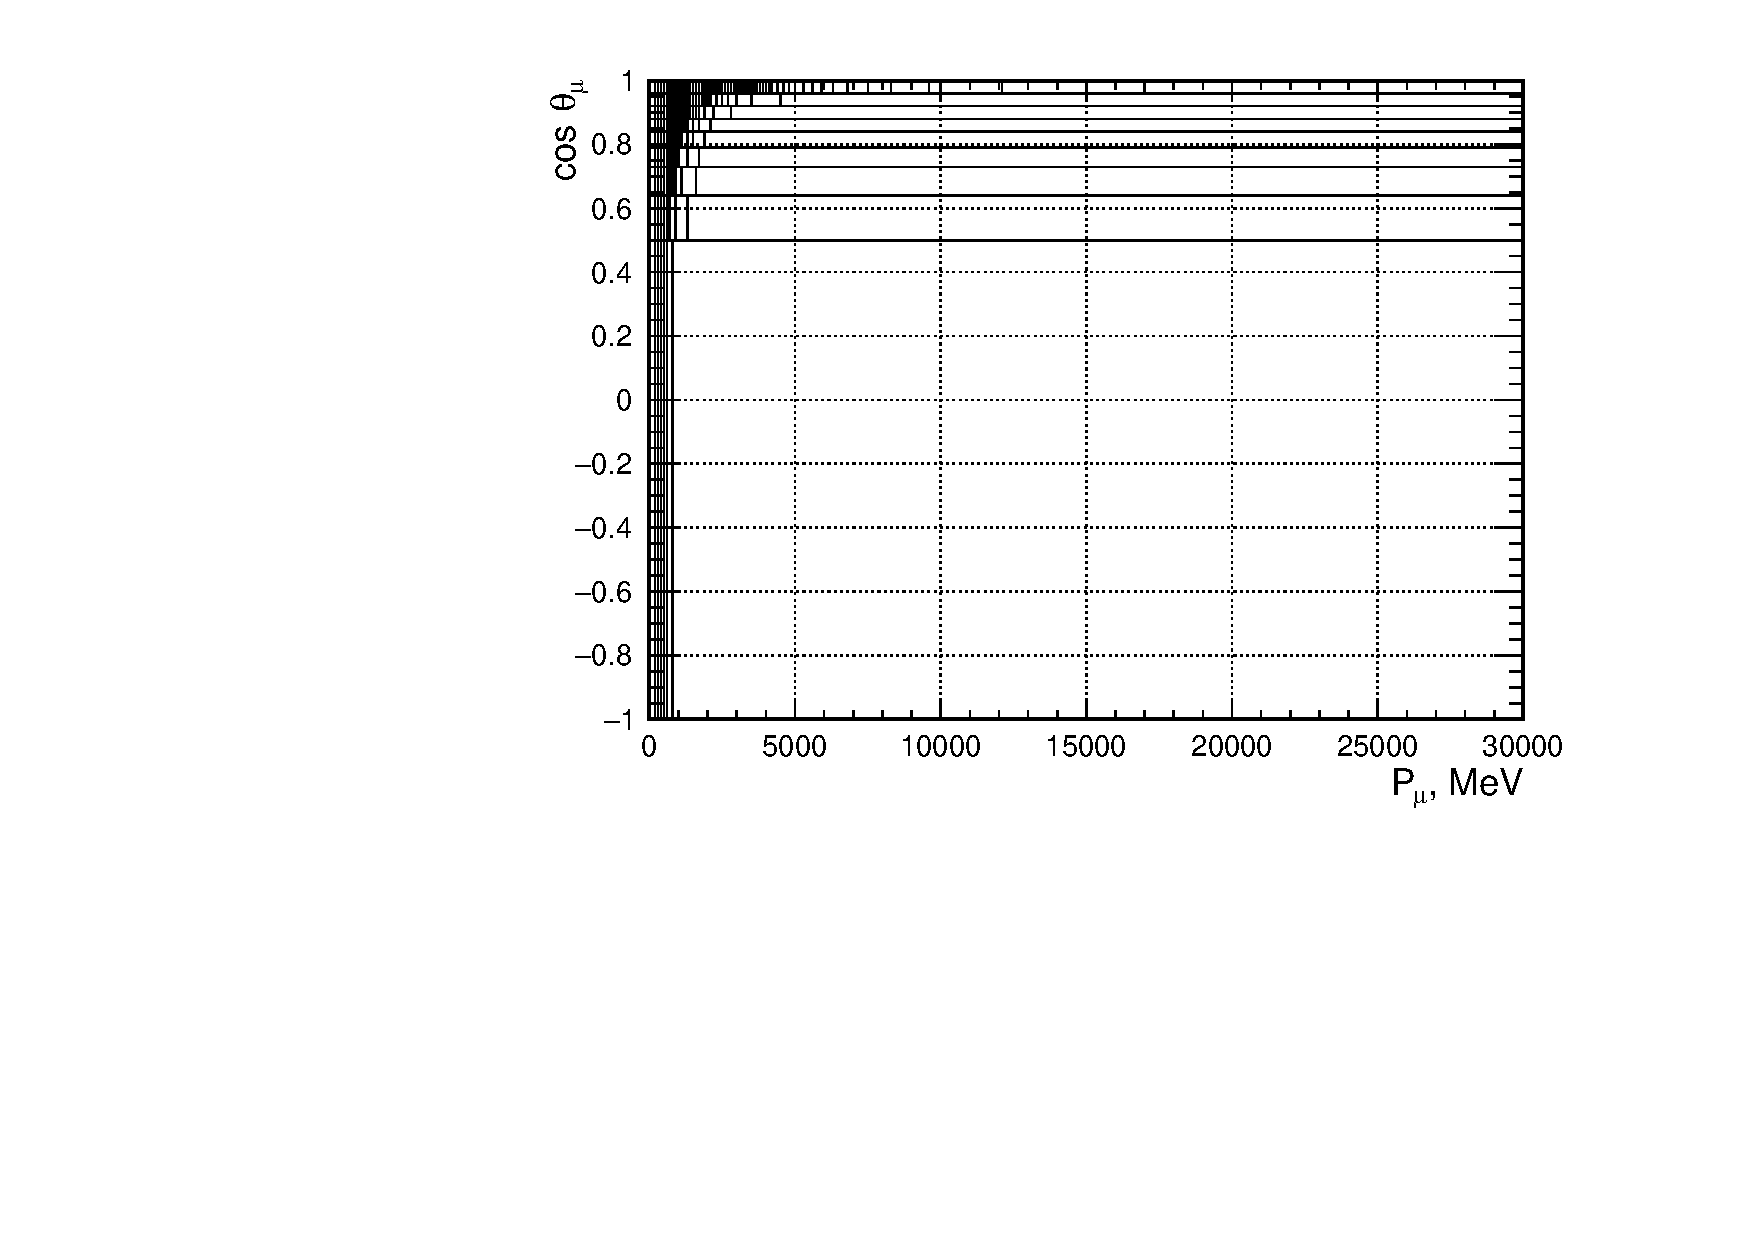
\includegraphics[width=0.95\linewidth]{figs/TH2PolyReset_MC_FGD2_anti-numuCC_0pi}
  \caption{FGD2 RHC $\bar{\nu_{\mu}}$ 0$\pi$}
  \label{fig:TH2Poly_ResetFGD2_anti-numuCC_0pi}
\end{subfigure}
\begin{subfigure}{.32\textwidth}
  \centering
  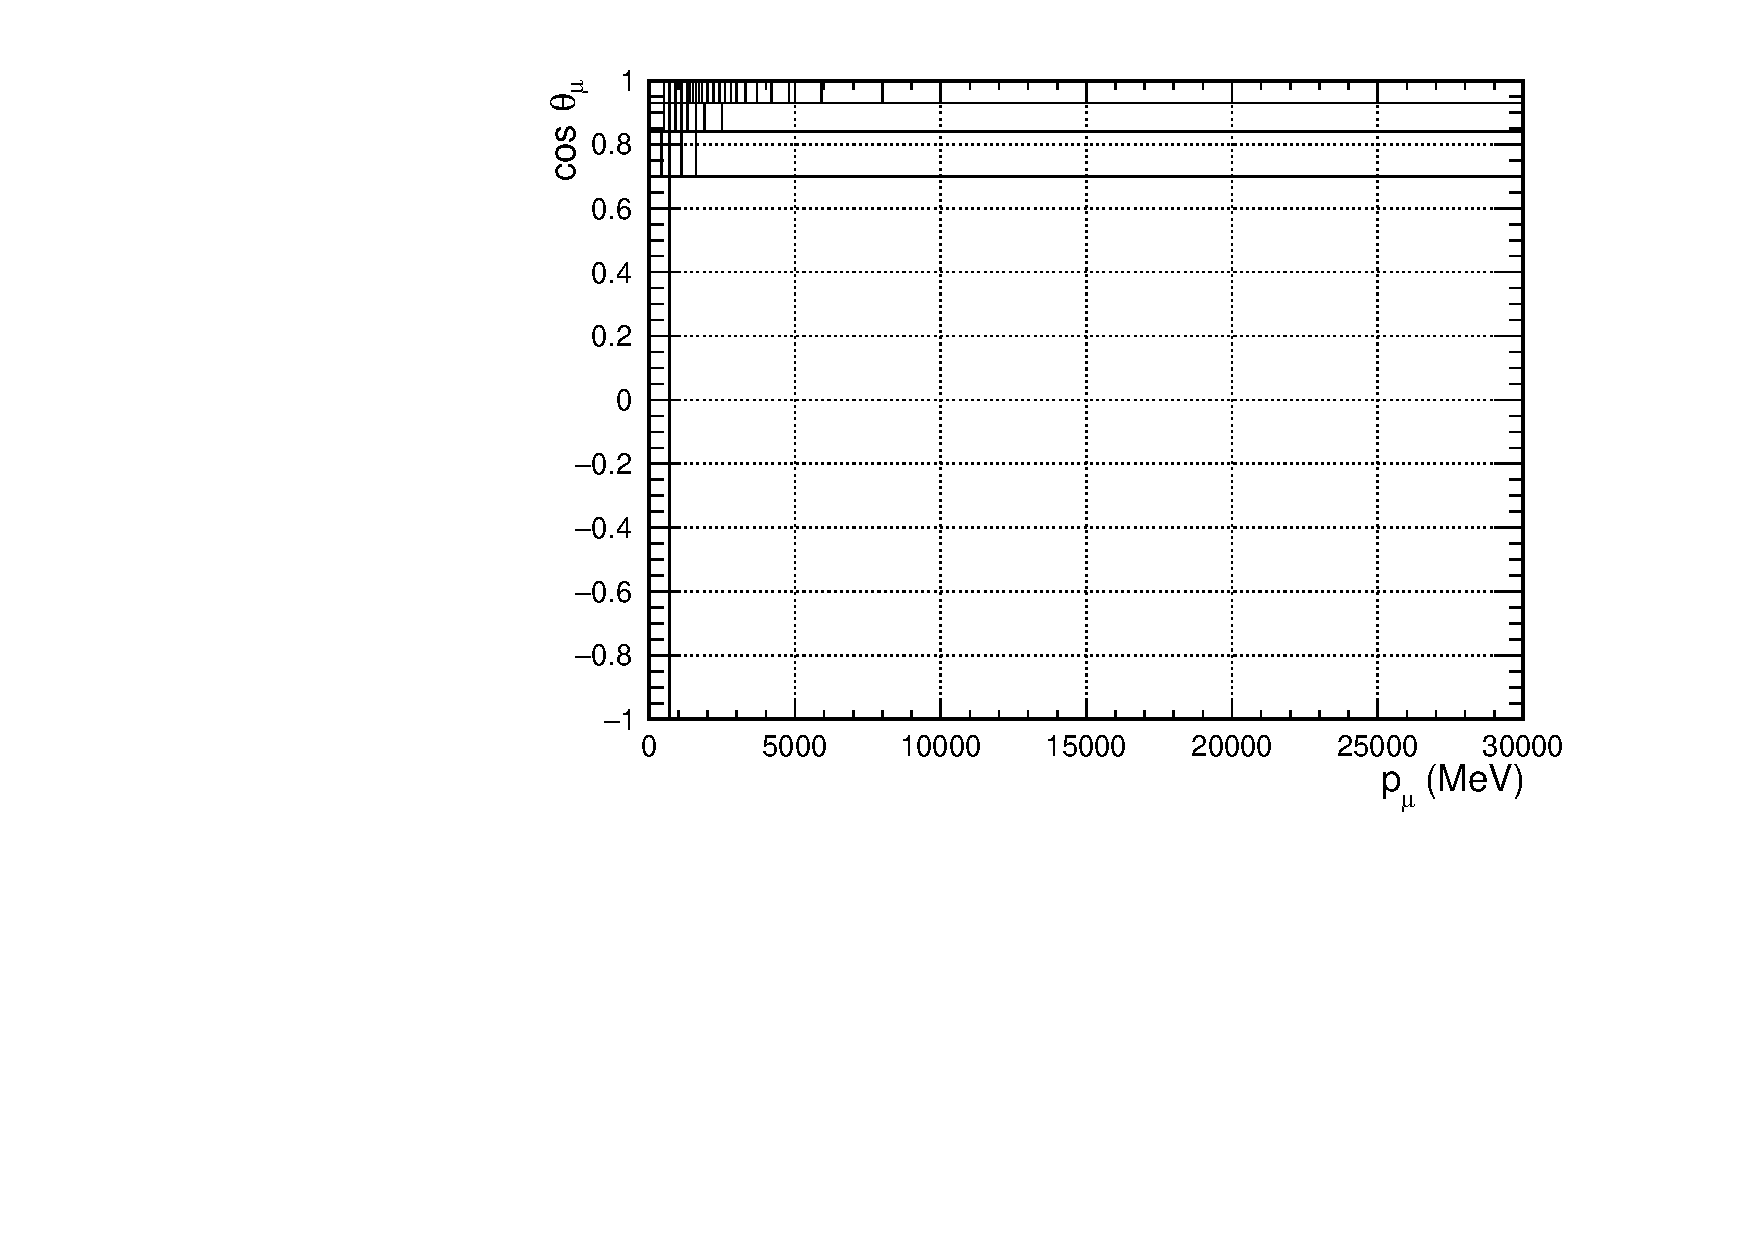
\includegraphics[width=0.95\linewidth]{figs/TH2PolyReset_MC_FGD2_anti-numuCC_1pi}
  \caption{FGD2 RHC $\bar{\nu_{\mu}}$ 1$\pi$}
  \label{fig:th2polyTH2Poly_ResetFGD2_anti-numuCC_1pi}
\end{subfigure}
\begin{subfigure}{.32\textwidth}
  \centering
  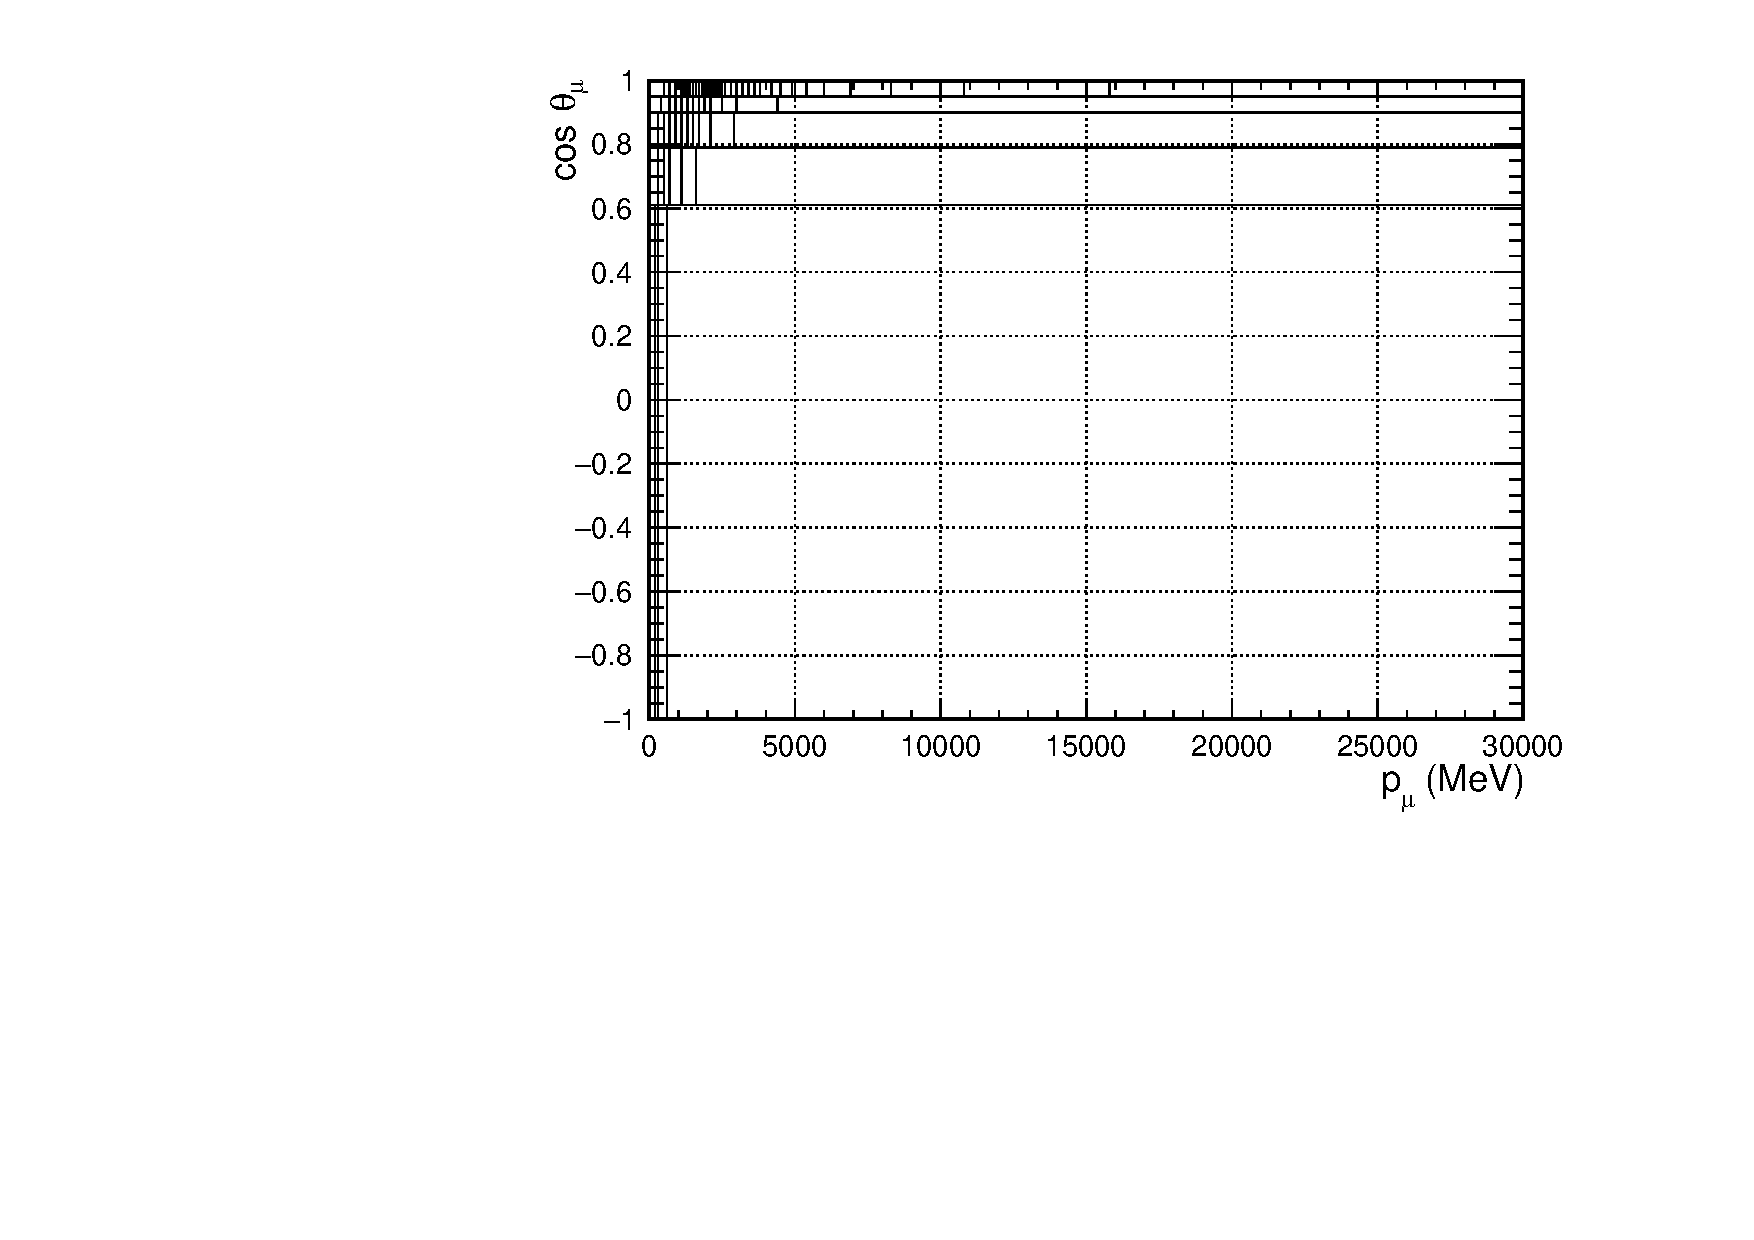
\includegraphics[width=0.95\linewidth]{figs/TH2PolyReset_MC_FGD2_anti-numuCC_other}
  \caption{FGD2 RHC $\bar{\nu_{\mu}}$ Other}
  \label{fig:TH2Poly_ResetFGD2_anti-numuCC_other}
\end{subfigure}
\begin{subfigure}{.32\textwidth}
  \centering
  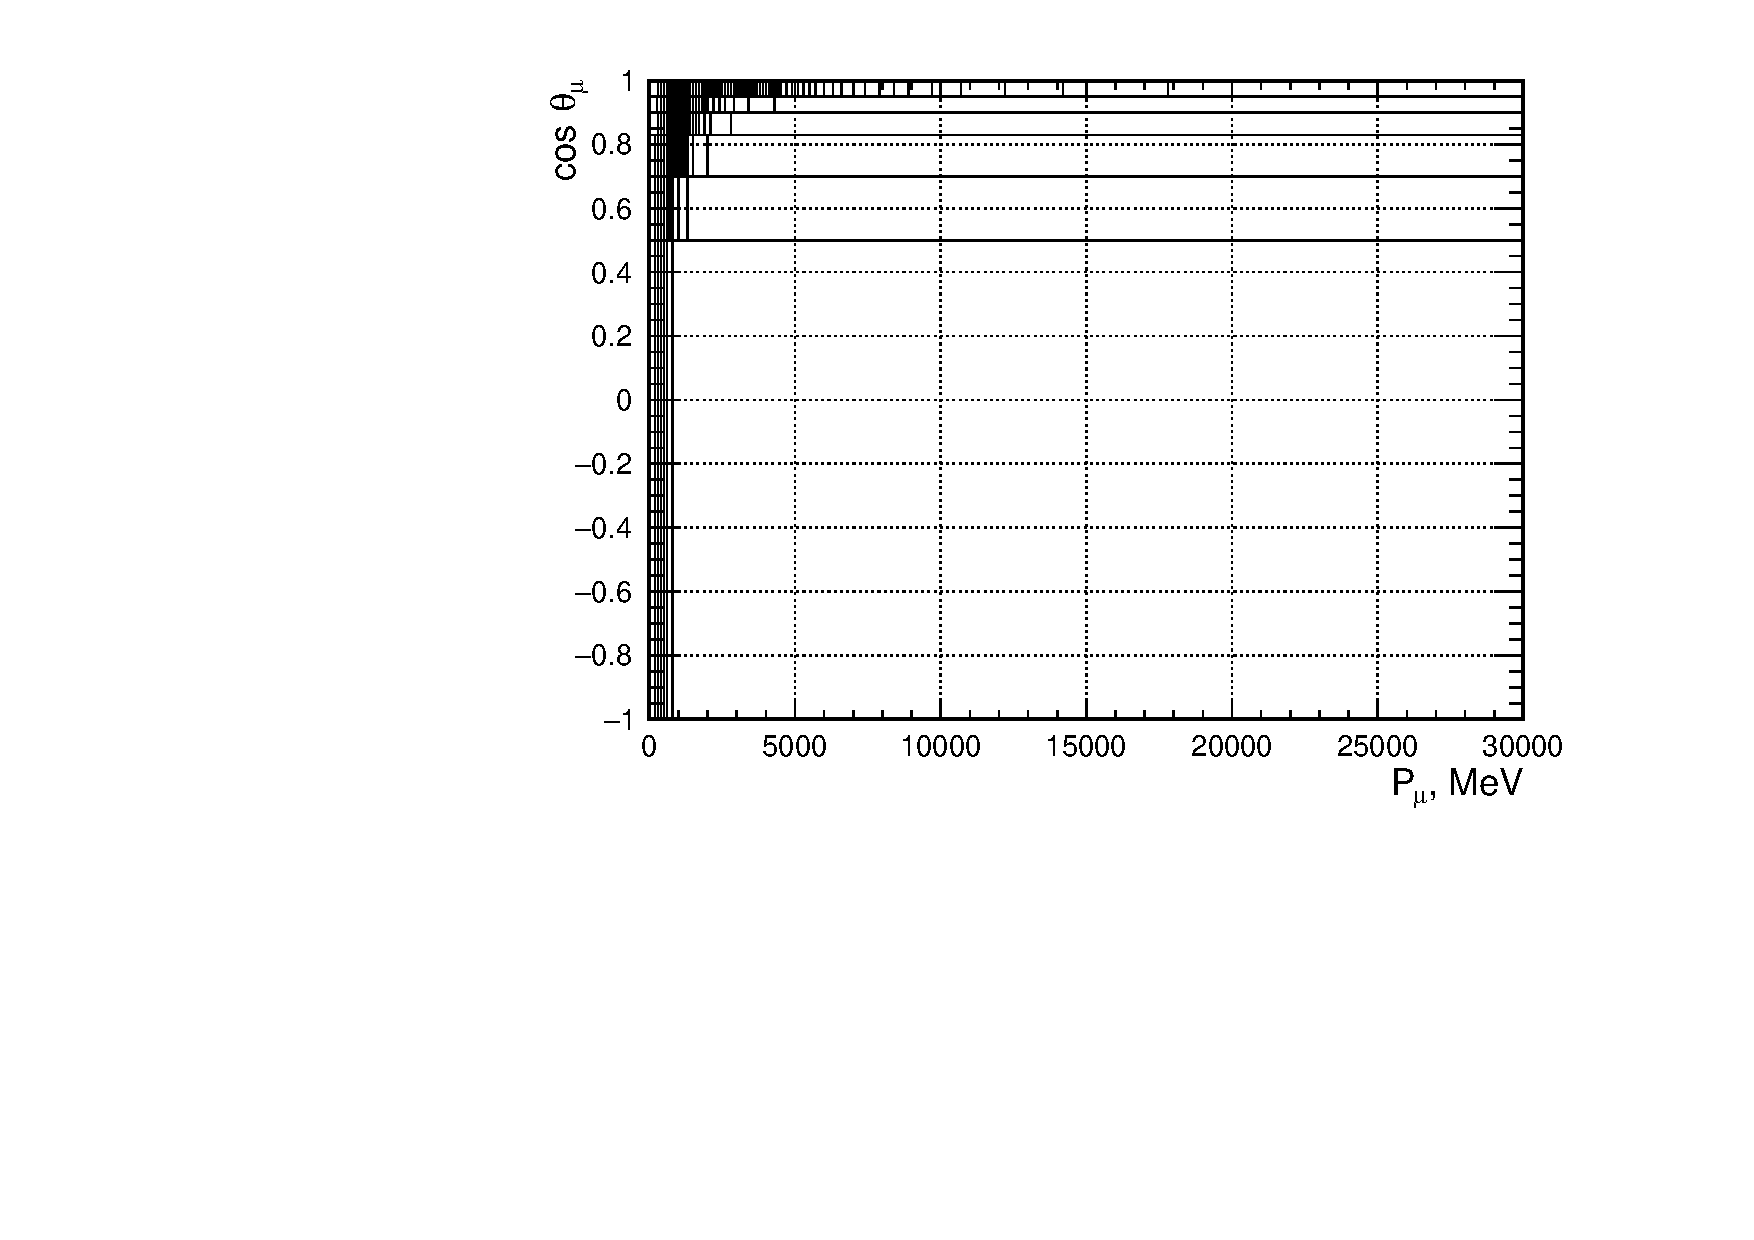
\includegraphics[width=0.95\linewidth]{figs/TH2PolyReset_MC_FGD1_NuMuBkg_CC0pi_in_AntiNu_Mode}
  \caption{FGD1 RHC $\nu_{\mu}$ 0$\pi$}
  \label{fig:TH2Poly_ResetFGD1_NuMuBkg_CC0pi_in_AntiNu_Mode}
\end{subfigure}
\begin{subfigure}{.32\textwidth}
  \centering
  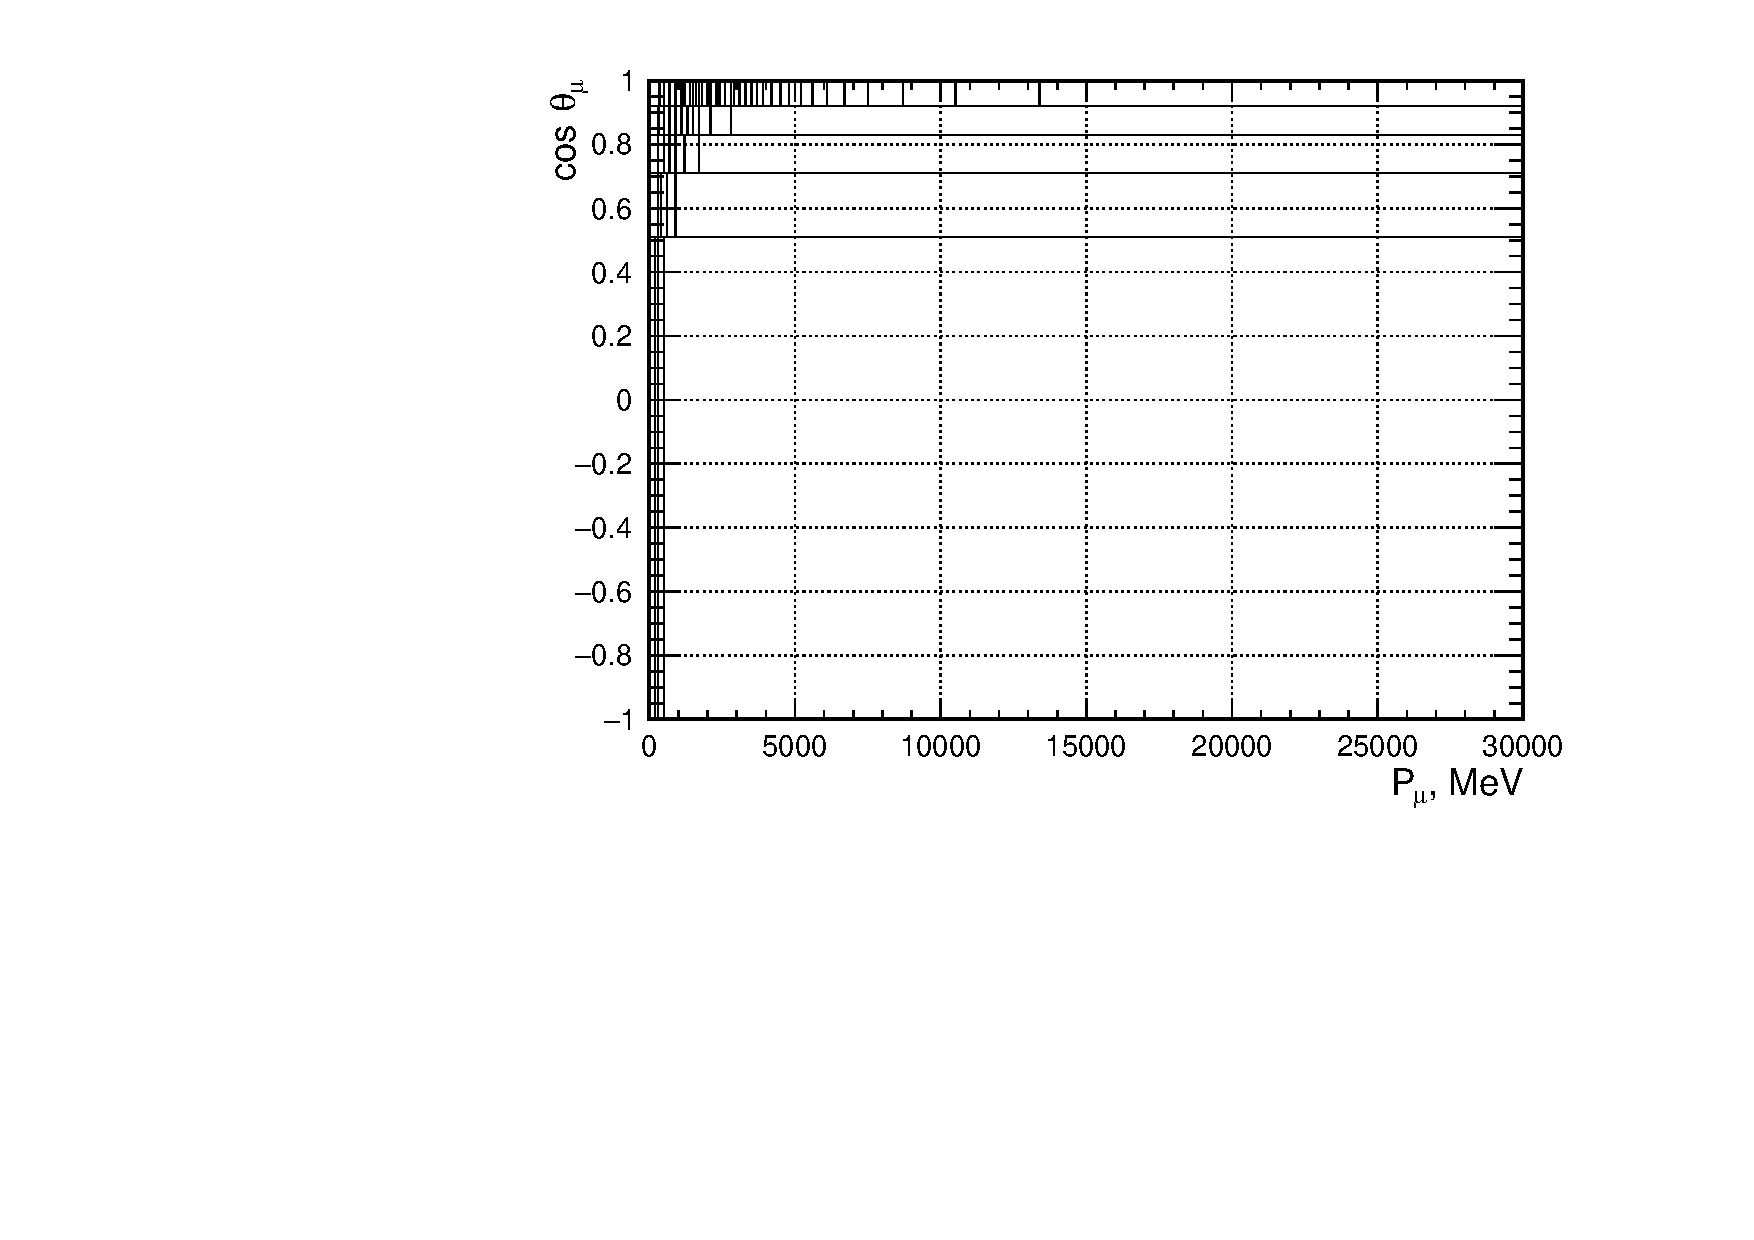
\includegraphics[width=0.95\linewidth]{figs/TH2PolyReset_MC_FGD1_NuMuBkg_CC1pi_in_AntiNu_Mode}
  \caption{FGD1 RHC $\nu_{\mu}$ 1$\pi$}
  \label{fig:TH2Poly_ResetFGD1_NuMuBkg_CC1pi_in_AntiNu_Mode}
\end{subfigure}
\begin{subfigure}{.32\textwidth}
  \centering
  \includegraphics[width=0.95\linewidth]{figs/TH2PolyReset_MC_FGD1_NuMuBkg_CCOther_in_AntiNu_Mode}
  \caption{FGD1 RHC $\nu_{\mu}$ Other}
  \label{fig:TH2Poly_ResetFGD1_NuMuBkg_CCOther_in_AntiNu_Mode}
\end{subfigure}
\begin{subfigure}{.32\textwidth}
  \centering
  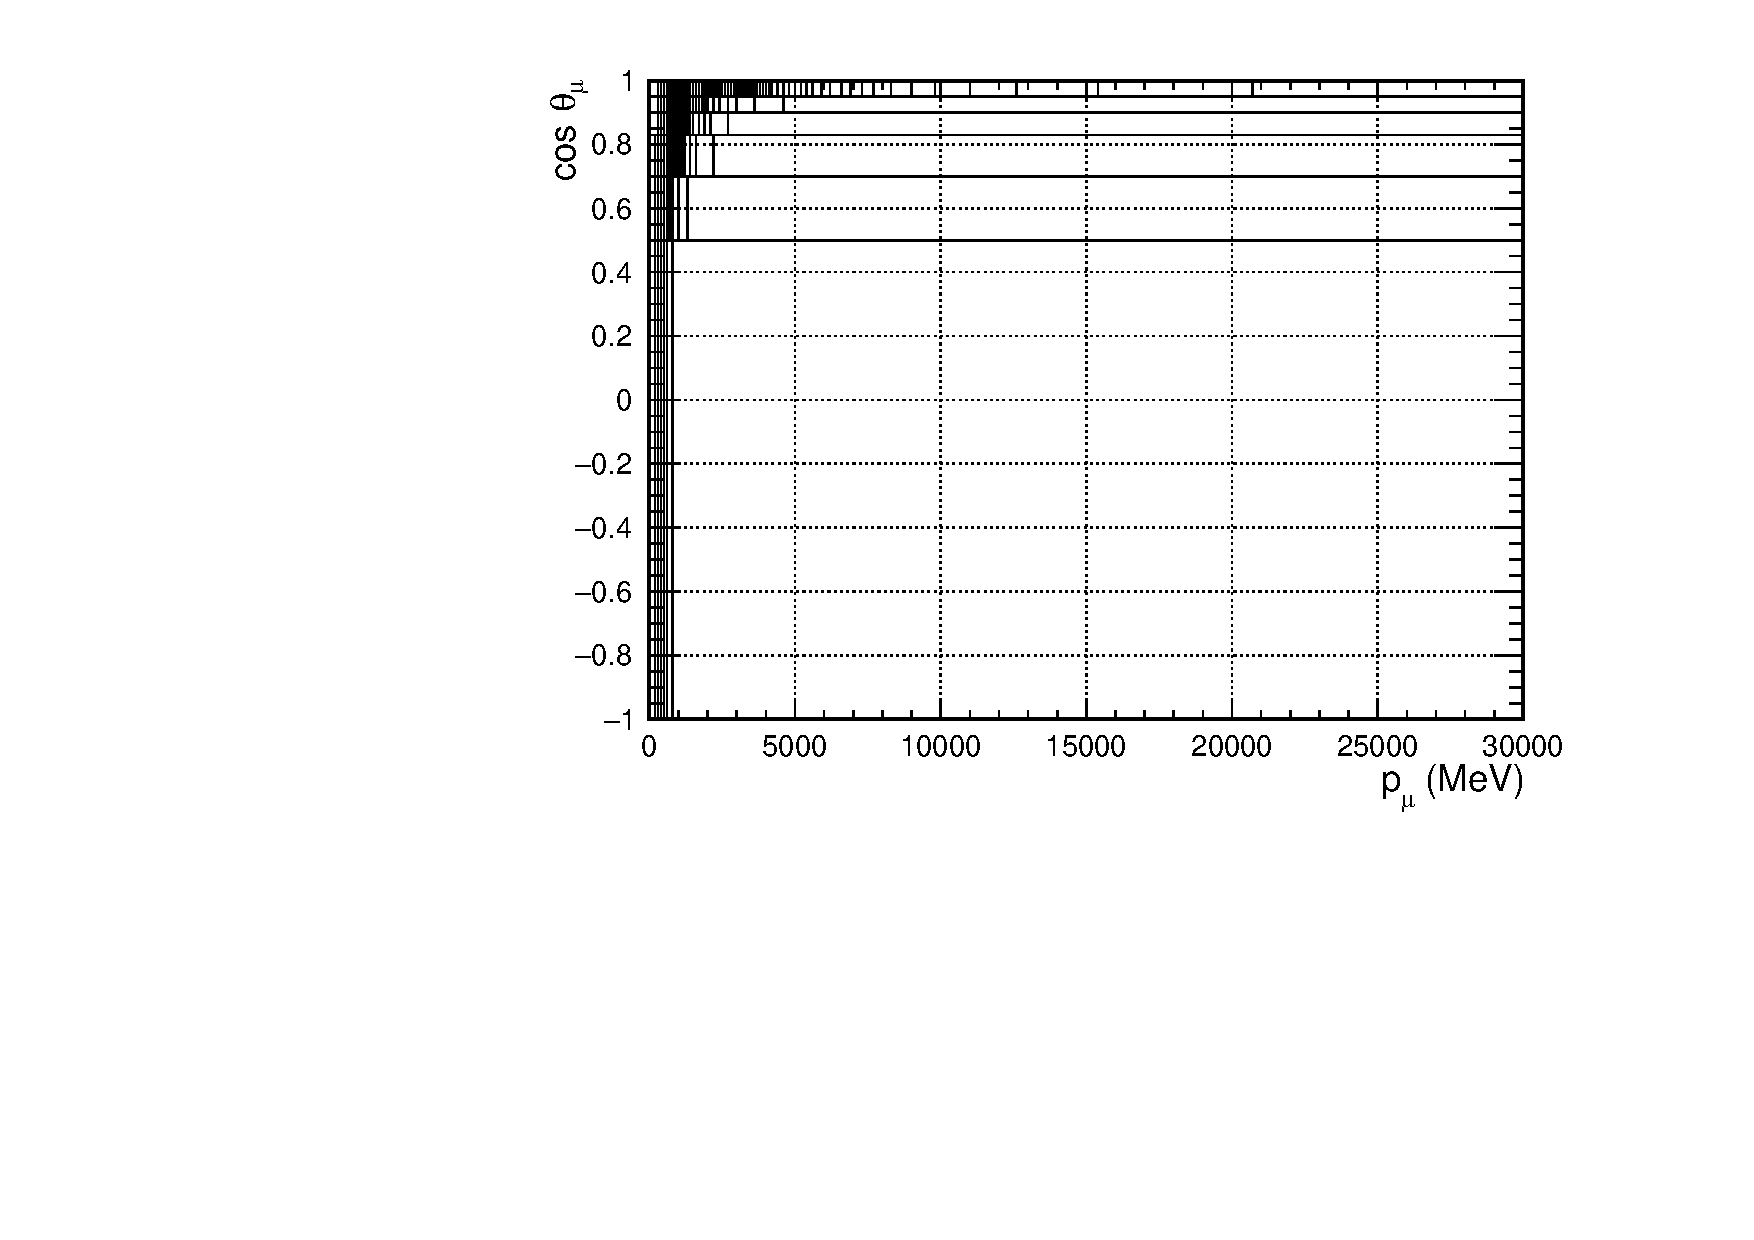
\includegraphics[width=0.95\linewidth]{figs/TH2PolyReset_MC_FGD2_NuMuBkg_CC0pi_in_AntiNu_Mode}
  \caption{FGD2 RHC $\nu_{\mu}$ 0$\pi$}
  \label{fig:TH2Poly_ResetFGD2_NuMuBkg_CC0pi_in_AntiNu_Mode}
\end{subfigure}
\begin{subfigure}{.32\textwidth}
  \centering
  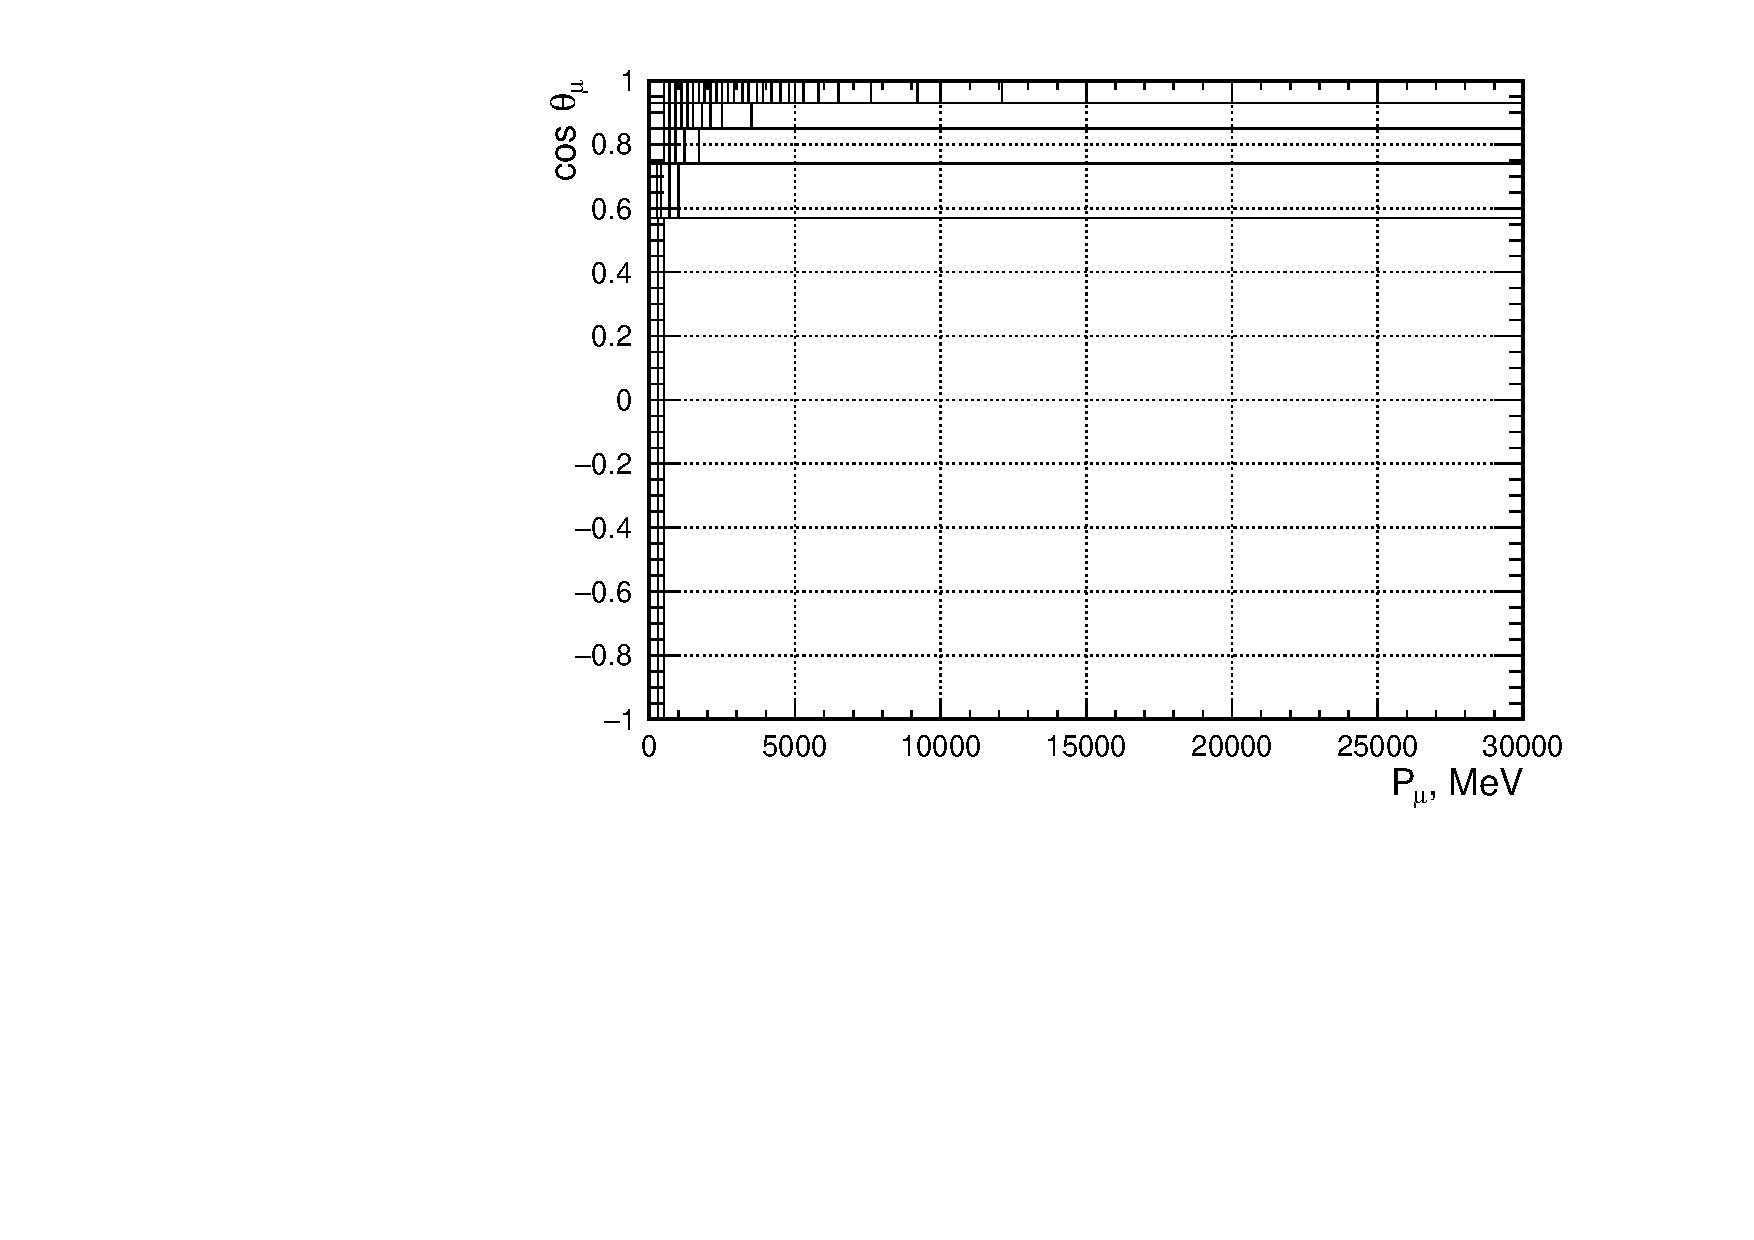
\includegraphics[width=0.95\linewidth]{figs/TH2PolyReset_MC_FGD2_NuMuBkg_CC1pi_in_AntiNu_Mode}
  \caption{FGD2 RHC $\nu_{\mu}$ 1$\pi$}
  \label{fig:TH2Poly_ResetFGD2_NuMuBkg_CC1pi_in_AntiNu_Mode}
\end{subfigure}
\begin{subfigure}{.32\textwidth}
  \centering
  \includegraphics[width=0.95\linewidth]{figs/TH2PolyReset_MC_FGD2_NuMuBkg_CCOther_in_AntiNu_Mode}
  \caption{FGD2 RHC $\nu_{\mu}$ Other}
  \label{fig:TH2Poly_ResetFGD2_NuMuBkg_CCOther_in_AntiNu_Mode}
\end{subfigure}
\caption{Non-uniform rectangular binning used in this analysis for each sample.}
\label{fig:th2polybinreset}
\end{figure}

The uniform binning used to validate against the other near detector fitting group is as follows:
\begin{itemize}

\item \textbf{FHC $\nu_{\mu}$ CC0$\pi$:}\\
\textbf{\textit{p} (MeV/c):} 0, 200, 300, 400, 450, 500, 550, 600, 650, 700, 750, 800, 850, 900, 950, 1000, 1050, 1100, 1200, 1300, 1400, 1500, 1600, 1700, 1800, 2000, 2500, 3000, 5000, 30000.\\
\textbf{cos $\theta$:} -1, 0.5, 0.6, 0.7, 0.76, 0.78, 0.8, 0.83, 0.85, 0.88, 0.89, 0.9, 0.91, 0.92, 0.925, 0.93, 0.935, 0.94, 0.945, 0.95, 0.955, 0.96, 0.965, 0.97, 0.975, 0.98, 0.985, 0.99, 0.995, 1.\\

\item \textbf{FHC $\nu_{\mu}$ CC1$\pi$:}\\
\textbf{\textit{p} (MeV/c):} 0, 300, 350, 400, 500, 600, 650, 700, 750, 800, 900, 1000, 1100, 1200, 1500, 2000, 3000, 5000, 30000.\\
\textbf{cos $\theta$:} -1, 0.6, 0.7, 0.8, 0.85, 0.88, 0.9, 0.92, 0.93, 0.94, 0.95, 0.96, 0.97, 0.98, 0.99, 0.995, 1.\\

\item \textbf{FHC $\nu_{\mu}$ CCOther:}\\
\textbf{\textit{p} (MeV/c):} 0, 300, 400, 500, 600, 650, 700, 750, 800, 900, 1000, 1100, 1250, 1500, 1750, 2000, 3000, 5000, 30000.\\
\textbf{cos $\theta$:} -1, 0.6, 0.7, 0.76, 0.8, 0.85, 0.88, 0.89, 0.9, 0.91, 0.92, 0.93, 0.94, 0.95, 0.96, 0.97, 0.98, 0.99, 0.995, 1.\\

\item \textbf{RHC $\bar{\nu}_{\mu}$ CC0$\pi$:}\\
\textbf{\textit{p} (MeV/c):} 0, 300, 400, 500, 550, 600, 650, 700, 750, 800, 900, 1000, 1100, 1200, 1500, 2000, 4000, 30000.\\
\textbf{cos $\theta$:} -1, 0.6, 0.7, 0.8, 0.85, 0.9, 0.92, 0.93, 0.94, 0.95, 0.96, 0.965, 0.97, 0.975, 0.98, 0.985, 0.99, 0.995, 1.\\

\item \textbf{RHC $\bar{\nu}_{\mu}$ CC1$\pi$:}\\
\textbf{\textit{p} (MeV/c):} 0, 500, 700, 900, 1300, 2500, 30000.\\
\textbf{cos $\theta$:}  -1, 0.7, 0.8, 0.9, 0.94, 0.96, 0.98, 0.99, 1.\\

\item \textbf{RHC $\bar{\nu}_{\mu}$ CCOther:}
\textbf{\textit{p} (MeV/c):} 0, 600, 800, 1000, 1250, 1500, 2000, 4000, 30000.\\
\textbf{cos $\theta$:} -1, 0.7, 0.8, 0.85, 0.9, 0.93, 0.95, 0.97, 0.98, 0.99, 1.\\

\item \textbf{RHC $\nu_{\mu}$ CC0$\pi$:}\\
\textbf{\textit{p} (MeV/c):} 0, 300, 500, 700, 800, 900, 1250, 1500, 2000, 4000, 30000.\\
\textbf{cos $\theta$:} -1, 0.7, 0.8, 0.85, 0.88, 0.9, 0.92, 0.94, 0.96, 0.97, 0.98, 0.99, 1.\\

\item \textbf{RHC $\nu_{\mu}$ CC1$\pi$:}\\
\textbf{\textit{p} (MeV/c):} 0, 600, 800, 1500, 30000.\\
\textbf{cos $\theta$:} -1, 0.7, 0.8, 0.86, 0.9, 0.94, 0.96, 0.97, 0.98, 0.99, 1.\\

\item \textbf{RHC $\nu_{\mu}$ CCOther:}\\
\textbf{\textit{p} (MeV/c):} 0, 600, 1000, 1250, 2000, 4000, 30000.\\
\textbf{cos $\theta$:} -1, 0.7, 0.8, 0.86, 0.9, 0.93, 0.95, 0.97, 0.99, 1.\\

\end{itemize}

\newpage